\documentclass[11pt]{article}
\usepackage{iftex}
\ifPDFTeX\usepackage[T1]{fontenc}\usepackage[utf8]{inputenc}\usepackage{lmodern}\else\usepackage{fontspec}\setmainfont{Latin Modern Roman}\fi
\usepackage{amsmath,amssymb,mathrsfs,booktabs,graphicx,hyperref}
\usepackage[margin=21.5mm]{geometry}
\hypersetup{hidelinks,pdftitle={Yang--Mills central signs and shrinking spectral windows}}
\allowdisplaybreaks
\emergencystretch=3em
\setlength{\parindent}{0pt}
\setlength{\parskip}{6pt}
\begin{document}
\section*{Original phase moments and the unchanged shrinking window}

This independent derivation uses the actual vacuum and original rooted
words throughout. Its original-path result is the explicit bound (IP8).
Its additional fixed-box results are (IP15)–(IP20). The fixed-box limits
do not establish the sign of the expression in (IP1) on the prescribed
joint path. No smaller selected coupling is substituted for that path.

\subsection*{1. Original objects and source locations}

The finite open box has vertex indices `(i,k,l)` in `\{0,...,m\}\textasciicircum{}3`, where
`m=2L`, `n=m+1`, and `L>=2`. The physical vertex remains
`o+a(i-L,k-L,l-L)`. It has
\[
 N=3m(m+1)^2,\qquad M=3m^2(m+1).
\]
The root is `(0,0,0)`. The root path goes in direction three, then two,
then one. The tree has every direction-one edge, direction-two edges
with first coordinate zero, and direction-three edges with first two
coordinates zero. For a chord `c=(s,t)`, retain the whole word
\(Z_c=t_sU_ct_t^{-1}\). No common segment is erased when occurrences
are counted below. The Lie generators are
\(T_\alpha=-i\sigma_\alpha/2\), and
\(q_c^\alpha=-2\operatorname{tr}(T_\alpha Z_c)\).

Write
\[
 h={\pi\over2n},\quad c=\cos h,\quad C=\cot h,\quad
 v_0(l)=n^{-1/2},\quad
 v(l)=\sqrt{2/n}\cos{\pi(l+1/2)\over n},\quad
 w(l)=-\sqrt{2/n}\sin{\pi(l+1)\over n}.
\]
The complete chord sets and the original first and third rows are
\[
\begin{split}
\mathcal C_2&=\{(i,k,l;2):1\le i\le m,\ 0\le k<m,\ 0\le l\le m\},\\
\mathcal C_3&=\{(i,k,l;3):0\le i,k\le m,\ (i,k)\ne(0,0),\ 0\le l<m\},\\
a_{(i,k,l;2)}&=-v(i)w(k)v_0(l)/\sqrt2,\qquad a_{(i,k,l;3)}=0,\\
b_{(i,k,l;2)}&=v_0(i)w(k)v(l)/\sqrt2,\\
b_{(i,k,l;3)}&=-v_0(i)v(k)w(l)/\sqrt2.
\end{split}
\]
Thus \(u_1=\sum_ca_cq_c\), \(u_3=\sum_cb_cq_c\),
\(\mathcal S=u_1\cdot u_3\), and
\(\mathcal S_{\mathcal R}=\mathcal S\circ\mathcal R\), with the
original direction-one graph reflection, all reversed edges and all
reflected root words. Put
\[
\sigma_*=\sqrt8\sin h,\quad \beta_0={\sigma_*\over2g^2},\quad
p=\beta_0\mathcal S,\quad r=\beta_0\mathcal S_{\mathcal R},\quad
F=p-r.
\]

The Hamiltonian and its actual positive unit vacuum are
\[
 H=\kappa H_0+bW,\quad H_0=-\sum_{e,\alpha}X_{e,\alpha}^2,
 \quad\kappa={2g^2\over a},\quad b={1\over2g^2a},\quad
 W=\sum_{\text{all faces }p}(2-\operatorname{tr}U_p),\quad H\psi=E_0\psi.
\]
In particular the constant \(2bM\) is retained in the potential and
vacuum equation. Let \(d\mu=\psi^2dU\), \(\mathcal A=H-E_0\),
\(G=\mu(F^2)\), \(C_F=\kappa\mu(|\nabla F|^2)\). Reflection makes
\(F\psi\) odd and vacuum orthogonal. The original expression is
\[
\begin{split}
\mathscr E(s)&=G-C_F/s\\
 &=2\beta_0^2(\mathcal Q_4-\mathcal Q_{4,\mathcal R})
 -{2\kappa\beta_0^2\over s}(\mathcal K_1-\mathcal K_{\mathcal R}),
\end{split}\tag{IP1}
\]
with every expectation and reflected gradient as in PK202.
The raw measure is
\(\nu_F(B)=\langle F\psi,\mathbf1_B(\mathcal A)F\psi\rangle\);
\(\nu_F((0,s])\ge\max\{0,\mathscr E(s)\}\).

The receiving source is the retained \href{https://github.com/KokunoYumeto/yang-mills-interacting-workbench/blob/485b61423c1f4e1805deb453c1b6b342b27842b6/yang-mills/continuations/20260930-s6-ns-moment-map-bridge/PERIOD_COUPLING_AND_PHYSICAL_KERNELS.md#L2440}{programme manuscript}, PK103–PK108, PK139,
PK143a–PK174, PK177a–PK177f, PK178–PK202 and PK207–PK227.
The cited proof edition is pinned at commit
`485b61423c1f4e1805deb453c1b6b342b27842b6`.
The fixed-box vacuum and cluster transport used in Section 4 is exactly
the retained \href{https://github.com/KokunoYumeto/yang-mills-interacting-workbench/blob/485b61423c1f4e1805deb453c1b6b342b27842b6/yang-mills/continuations/20260930-s6-ns-moment-map-bridge/PERIOD_COUPLING_AND_PHYSICAL_KERNELS.md#L2480}{PK104–PK105} and \href{https://github.com/KokunoYumeto/yang-mills-interacting-workbench/blob/485b61423c1f4e1805deb453c1b6b342b27842b6/yang-mills/continuations/20260930-s6-ns-moment-map-bridge/PERIOD_COUPLING_AND_PHYSICAL_KERNELS.md#L2632}{PK112}. It is not asserted to be
uniform in the box. The weighted-tail input is proved again in Section 3
from retained \href{https://github.com/KokunoYumeto/yang-mills-interacting-workbench/blob/485b61423c1f4e1805deb453c1b6b342b27842b6/yang-mills/continuations/20260930-s6-ns-moment-map-bridge/sources/spatial/spatial_continuum.tex#L3875}{original TeX, equations (205)–(214), Section 17.4–17.5}. Both pinned files were retrieved and matched byte for byte to the local files used here. Source identities and reading coverage are in the
separate source ledger; index hits are not reading evidence.

\subsection*{2. Exact original-word sums and an actual-vacuum endpoint bound}

Let \(n_{ce}\) count both orientations of link \(e\) in the full
word \(Z_c\). Put
\[
 S_1=\sum_c|a_c|=\sqrt{2/n}\,C(C-c),\qquad
 S_3=\sum_c|b_c|=\sqrt{2/n}[(2-1/n)C^2-(c/n)C].
\]
These are the complete PK162 sums. Define, without changing them,
\[
 D_{1e}=\sum_c|a_c|n_{ce},\quad D_{3e}=\sum_c|b_c|n_{ce},\quad
 K_e=2S_3D_{1e}+2S_1D_{3e},\quad
 \mathcal C=3\sum_eK_e^2.\tag{IP2}
\]
The three colours and all original physical links remain in this sum.
PK151–PK153 give pointwise \(|\nabla\mathcal S|^2\le\mathcal C\).

For either chord based at `(i,k,l)`, its original length is
\(\ell_c=2(i+k+l+1)\). For a direction-two chord the two root paths
share exactly \(k+l\) physical edges; for a direction-three chord they
share exactly \(l\). A shared edge occurs twice, once in each root
path; every other root edge and the chord occur once. Consequently
\[
\begin{array}{c|cc}
 &\sum_en_{ce}&\sum_en_{ce}^2\\ \hline
c\in\mathcal C_2&2(i+k+l+1)&2i+4k+4l+2\\
c\in\mathcal C_3&2(i+k+l+1)&2i+2k+4l+2.
\end{array}\tag{IP3}
\]
This calculation preserves the repeated root occurrences. The count
\(\sum n^2\) differs from \(\sum n\) precisely by twice the number
of shared edges, because \(2^2-2=2\).

Define \(L_\mu=\sum_c|\mathsf M_{\mu c}|\ell_c\) and
\(A_\mu=\sum_c|\mathsf M_{\mu c}|\sum_en_{ce}^2\), for \(\mu=1,3\).
Their exact values are
\[
\begin{split}
 L_1&=\sqrt{2/n}\,C[(3m+1)C-(2m+1)c],\\
 L_3&=\sqrt{2/n}[(6m+1/n)C^2-cC],\\
 A_1&=m\sqrt{2/n}\,C(5C-4c),\\
 A_3&={m\over n}\sqrt{2/n}[(9m+5)C^2-2cC].
\end{split}\tag{IP4}
\]
Here \(A_\mu\) are occurrence sums; they are unrelated to the
amplitude parameter or the operator \(\mathcal A\).

For a full summation proof, set
\(V=\sum_{i=0}^m|v(i)|=\sqrt{2/n}C\),
\(V_0=\sum_{i=1}^m|v(i)|=\sqrt{2/n}(C-c)\), and
\(W_1=\sum_{k=0}^{m-1}|w(k)|=\sqrt{2/n}C\).
Reflection gives the first absolute moments
\[
\sum_{i=0}^m i|v(i)|={mV\over2},\quad
\sum_{k=0}^{m-1}k|w(k)|={(m-1)W_1\over2},\quad
\sum_{i=0}^m i={mn\over2}.
\]
Removing \(i=0\) from the first moment leaves its numerator unchanged.
Thus the first-row averages of `(i,k,l)` are
\(mC/[2(C-c)],(m-1)/2,m/2\). Inserting these into (IP3)
gives both first-row formulas in (IP4).

The third row's direction-two absolute mass is
\(S_{3,2}=\sqrt{2/n}(m/n)C^2\), and the corresponding coordinate
averages are \((m+1)/2,(m-1)/2,m/2\). Its contributions to
\(L_3,A_3\) are respectively \((3m+2)S_{3,2}\) and
\((5m+1)S_{3,2}\).
The unexcluded direction-three rectangle has mass
\(S_{3,3}^{\rm all}=\sqrt{2/n}C^2\), coordinate averages
\(m/2,m/2,(m-1)/2\), and contributions
\((3m+1)S_{3,3}^{\rm all},4mS_{3,3}^{\rm all}\).
Its excluded corner `(i,k)=(0,0)` has mass
\(X=\sqrt{2/n}(cC/n)\), length average \(m+1\) and squared-occurrence
average \(2m\). Subtracting exactly \((m+1)X,2mX\), respectively,
gives the two third-row formulas in (IP4), including every endpoint.

Cauchy–Schwarz with the original absolute coefficient measure gives
\[
 \sum_eD_{\mu e}^2
 \le S_\mu\sum_c|\mathsf M_{\mu c}|\sum_en_{ce}^2=S_\mu A_\mu.
\]
The triangle inequality in the finite link Euclidean space, applied
to (IP2), now proves the full explicit bound
\[
\boxed{\quad
\mathcal C\le\mathcal C_{\rm occ}:=
12\left[S_3\sqrt{S_1A_1}+S_1\sqrt{S_3A_3}\right]^2.
\quad}\tag{IP5}
\]
There is also the independent length bound
\[
 \mathcal C\le48S_1S_3(S_3L_1+S_1L_3).\tag{IP6}
\]
Indeed \(0\le n_{ce}\le2\) implies
\(K_e\le8S_1S_3\), while
\(\sum_eK_e=2S_3L_1+2S_1L_3\); multiply these and then by three.
Both bounds are for the same full occurrence sum, not reduced words.

Since reflection is unitary for the actual vacuum energy form,
\(\|\nabla(\mathcal S-\mathcal S_{\mathcal R})\|_{L^2(\mu)}^2
\le4\|\nabla\mathcal S\|_{L^2(\mu)}^2\).
For detail, its even and odd parts are form orthogonal: applying
reflection changes the cross term's sign while preserving its value.
The odd projection therefore contracts the form, and
\(\mathcal S-\mathcal S_{\mathcal R}=2P_-\mathcal S\).
The same argument in norm and \(|u_\mu|\le2S_\mu\) prove
\[
0<G\le64\beta_0^2S_1^2S_3^2,\qquad
0<C_F\le4\kappa\beta_0^2\mathcal C_{\rm occ}.\tag{IP7}
\]
Strict positivity is the finite-regulator PK202 statement. No positive
lower bound uniform in the regulator has been inserted.

On precisely the requested path, for integers \(j\ge2\),
\[
 L_j=j^4,\quad a_j={1\over100j},\quad
 g_j^2={\kappa_*\over200j},\quad s_j={\kappa_*\over j},\quad
 m_j=2j^4,\quad n_j=2j^4+1,\quad
 \beta_{0,j}={200\sqrt2j\over\kappa_*}\sin{\pi\over4j^4+2},
\]
the actual expression (IP1) obeys
\[
\boxed{
 -4j\beta_{0,j}^2\mathcal C_{{\rm occ},j}
 \ \le\ \mathscr E_j(s_j)
 \ \le\ 64\beta_{0,j}^2S_{1,j}^2S_{3,j}^2.
}\tag{IP8}
\]
Every quantity at the endpoints is the displayed finite trigonometric
formula. This is a direct bound on the actual-vacuum expression, without
an electric cutoff or a change of vector.

For its exact growth constants, let \(\tau=19/2+3\sqrt{10}\).
The finite formulas give
\[
\begin{gathered}
 {S_1\over n^{3/2}}\to{4\sqrt2\over\pi^2},\quad
 {S_3\over n^{3/2}}\to{8\sqrt2\over\pi^2},\quad
 {A_1\over nS_1}\to5,\quad {A_3\over nS_3}\to{9\over2},\\
 {\mathcal C_{\rm occ}\over n^7}\to{49152\tau\over\pi^8},\quad
 {\mathcal C_{\rm occ}\over192NS_1^2S_3^2}\,n^2\to{\tau\over48},\\
 {4j\beta_{0,j}^2\mathcal C_{{\rm occ},j}\over j^{23}}
 \to {125829120000\tau\over\kappa_*^2\pi^6},\\
 {64\beta_{0,j}^2S_{1,j}^2S_{3,j}^2\over j^{18}}
 \to {83886080000\over\kappa_*^2\pi^6}.
\end{gathered}\tag{IP9}
\]
For example, the first line follows from \(C/n\to2/\pi\), \(c\to1\)
in (IP4), with no finite term removed. Substitution into (IP5) gives
\(12\cdot4096(\sqrt5+3/\sqrt2)^2/\pi^8\), the second line.
Then \(n_j/j^4\to2\) and
\(j^6\beta_{0,j}^2\to5000\pi^2/\kappa_*^2\) give the last lines.
The earlier bound PK177 grows as \(n^9\); (IP5) grows as \(n^7\).
Thus the negative loss bound improves by eight powers of \(j\).
Its sign remains negative and its magnitude grows. This result does
not prove positivity, decay, or growth of the actual expression itself.

\subsection*{3. The next calculation: control the unbounded phase moments}

The obstacle to using PK148 for \(F=p-r\) is that \(p,r\) contain
\(g^{-2}\). Strong convergence of the vacuum alone does not control
these multipliers. We now calculate the needed tails from the actual
vacuum equation.

For a face set \(D_p=2-\operatorname{tr}U_p\), so \(W=\sum_pD_p\).
Holding the other links fixed and writing the face product as a unit
quaternion gives
\(\sum_\alpha|X_{e,\alpha}D_p|^2=D_p-D_p^2/4\le D_p\)
for every incident link. Conjugations preserve the three-colour norm;
inverse traversals give the same result by the original bi-invariant
metric. Each edge has \(r_e\le4\) incident faces, and every face has
four edges. Cauchy–Schwarz over its incident faces therefore gives
\(|\nabla W|^2\le16W\), including the boundary.

For any real smooth multiplier \(f\), expansion of all product
derivatives and Haar integration by parts yield
\[
 q_H[f\psi]-E_0\mu(f^2)=\kappa\mu(|\nabla f|^2).
\]
The potential and its constant are retained until the vacuum equation
is inserted. The kinetic term in \(q_H\) is nonnegative. With
\(M_k=\mu(W^k)\), \(M_0=1\), this implies
\[
 bM_{k+1}\le E_0M_k+4\kappa k^2M_{k-1}\quad(k\ge1),\qquad
 M_1\le E_0/b.
\]
For \(k=1\), use \(f=(W+\epsilon)^{1/2}\), whose gradient square
is at most four, and pass to \(\epsilon\downarrow0\). For every
higher odd power use the same positive regularization; compactness
and the bound on \(|\nabla W|^2\) justify convergence. For even powers
ordinary differentiation suffices. The retained variational bound is
\(E_0\le K=3\sqrt{NM}/a\), at every positive coupling. Thus, with
\(U_g=W/g^2\),
\[
\begin{gathered}
 \mu(U_g^k)\le B_k,\quad
 B_0=1,\quad B_1=6\sqrt{NM},\quad
 B_{k+1}=6\sqrt{NM}B_k+16k^2B_{k-1},\\
 B_2=36NM+16,\qquad
 B_3=216(NM)^{3/2}+480\sqrt{NM}.
\end{gathered}\tag{IP10}
\]
All factors here come from the original \(b,\kappa,a,g\).

The ordered non-Abelian face fillings PK177a–PK177e give the pointwise
bound \(|u_\mu|^2\le4T_\mu w_\mu W\), where
\[
 T_1={mC^2\over\sqrt{2n}},\quad T_3=3T_1,\quad
 w_1={\sqrt2c(C-c)\over n^{3/2}},\quad w_3=nw_1.
\]
It follows that, with \(P_{\rm fill}=T_1T_3w_1w_3\),
\[
 |\mathcal S|\le4\sqrt{P_{\rm fill}}\,W,\quad
 |\mathcal S_{\mathcal R}|\le4\sqrt{P_{\rm fill}}\,W,\quad
 |p|,|r|\le2\sigma_*\sqrt{P_{\rm fill}}\,U_g,\quad
 |F|^2\le16\sigma_*^2P_{\rm fill}\,U_g^2.\tag{IP11}
\]
Reflection preserves the whole potential \(W\); that is why the same
constant applies to its full reflected word.

There is an equally explicit derivative domination. Set
\[
 D_W=12\sum_e
 \left[\sqrt{T_3w_3}D_{1e}+\sqrt{T_1w_1}D_{3e}\right]^2.
\]
For each of the three generators,
\(|X\mathcal S|\le|u_3|D_{1e}+|u_1|D_{3e}\).
Square the face bounds and sum all generators to obtain
\[
\begin{gathered}
 |\nabla\mathcal S|^2\le D_W W,\qquad
 |\nabla(\mathcal S-\mathcal S_{\mathcal R})|^2\le4D_WW,\\
 \kappa|\nabla p|^2,\ \kappa|\nabla r|^2
       \le{\sigma_*^2D_W\over2a}U_g,\qquad
 \kappa|\nabla F|^2\le{2\sigma_*^2D_W\over a}U_g,\\
 D_W\le12\left[
 \sqrt{T_3w_3S_1A_1}+\sqrt{T_1w_1S_3A_3}\right]^2.
\end{gathered}\tag{IP12}
\]
For the second bound use \(|v-w|^2\le2|v|^2+2|w|^2\)
and reflection invariance of the pointwise metric and \(W\).
The last bound follows from the same finite-link Cauchy–Schwarz as
(IP5). These are actual all-coupling bounds for the original global
functions, including the region beyond a logarithm chart.

At fixed box, the chord potential vanishes only at the identity chord
configuration. To verify this, every rooted chord is the ordered product
of conjugates of the faces in its filling; if every face is identity,
so is every chord. Conversely identity chords are flat. Its quadratic
form there is \(\frac14\sum_\alpha\|Cy^\alpha\|^2\), with
\(C^*C>0\) on the chord coordinates. Therefore a radius \(\rho>0\)
and positive constants \(c_*,c_\rho\) exist such that
\(W(y)\ge c_*|y|^2\) when \(|y|<\rho\), and
\(W\ge c_\rho\) outside that neighborhood. Positivity of the first
constant follows from the least eigenvalue and the Taylor remainder;
positivity of the second follows by compactness and the just-proved
unique zero. They depend on this fixed box.

For the exact transported coordinate \(y=gx\), any integer \(k\ge0\)
satisfies
\[
 \int_{|x|>R} U_g^k\,|\mathcal B_g\psi_g|^2dx
 \le B_{k+1}\left({1\over c_*R^2}+{g^2\over c_\rho}\right).
 \tag{IP13}
\]
The notation in this equation means multiplication by
\(U_g(\exp(gx))\) inside the exact density/dilation transport;
the integrand is zero outside its original domain \(\Omega_g\).
On the part \(|gx|<\rho\), \(U_g\ge c_*R^2\), so
\(U_g^k\le U_g^{k+1}/(c_*R^2)\). On the other part
\(U_g\ge c_\rho/g^2\), and use the other summand. (IP10)
and the exact isometry prove (IP13).

\subsection*{4. Exact fixed-box phase matrices and their degeneration}

Use the exact retained coordinate maps
\(z^\alpha=O^{\mathsf T}G_{\rm kin}^{-1/2}x^\alpha\), where here
\(G_{\rm kin}=TT^*\) is the original quotient kinetic matrix (not the
scalar raw norm \(G\) in (IP1)). No constant-Jacobian map is suppressed:
it is the unitary coordinate change already specified in PK103–PK105.
The symbol \(G_{\rm kin}\) will denote this same matrix below.
The actual vacuum transport converges strongly to the original Gaussian
\(\Phi_0\). The first and third selected modes have component variance
\(2/\sigma_*\) and are independent. Put
\[
 q_0(z)={\sigma_*\over2}z_1\cdot z_3,\qquad
 \delta_*={2\sigma_*\over a}.
\]
The local exact word expansion gives, together with every first
derivative on compact sets,
\[
 p(\exp(gx))\longrightarrow q_0(z),\qquad
 r(\exp(gx))\longrightarrow-q_0(z).\tag{IP14}
\]
Indeed \(q_c(\exp(gx))=g x_c+O(g^3|x_c|^3)\) locally;
the original reflected chord map has derivative taking the first mode
to its negative and the third to itself. Its nonlinear remainder is
retained until the limit, and differentiation of its analytic word
formula has the corresponding locally uniform remainder.

For every fixed polynomial \(P(x,y)\), (IP11), (IP10), and (IP13)
prove
\[
 \mathcal B_g[P(p,r)\psi_g]
       \longrightarrow P(q_0,-q_0)\Phi_0
       \quad\hbox{strongly in }L^2,\qquad g\downarrow0
       \quad(L,a\hbox{ fixed}).\tag{IP15}
\]
Here is the full tail argument. Each degree-\(d\) monomial is bounded
in absolute value by \((2\sigma_*\sqrt{P_{\rm fill}})^d U_g^d\),
using the exact scalar \(P_{\rm fill}=T_1T_3w_1w_3\) from (IP11).
For a polynomial, sum its finitely many such bounds and square using
finite Cauchy–Schwarz. Formula (IP13) with powers up to \(2d\), hence
the actual moment bounds up to \(B_{2d+1}\), makes its transported
squared tails uniformly small by first taking \(g\downarrow0\),
then \(R\to\infty\). On a fixed ball, (IP14) gives uniform multiplier
convergence, and the actual vacuum converges strongly. The limit is a
polynomial times a Gaussian and has an integrable squared tail. Adding
the ball and its two tails proves (IP15).

The actual energy forms of any two fixed such polynomials also converge.
The gradient of a constant monomial is zero. To verify the other tails,
for a degree-\(d\ge1\) monomial its gradient is a sum
of \(d\) terms, each consisting of a phase gradient times \(d-1\)
phase factors. The complete two-phase chain rule and (IP11)–(IP12)
bound its \(\kappa|\nabla\cdot|^2\) by a finite fixed-box constant
times \(U_g^{2d-1}\). Mixed products follow by Cauchy–Schwarz. (IP13)
therefore controls every energy tail as well, using one more actual
moment. On a fixed ball the original quotient fields have coefficient
matrix tending to \(G_{\rm kin}\otimes I_3\) and
\(\kappa=2g^2/a\); the derivative dilation supplies \(g^{-2}\).
Thus the exact limiting form is
\((2/a)\int\sum_\alpha(\nabla_{x^\alpha}f)^*
G_{\rm kin}\nabla_{x^\alpha}h\,|\Phi_0|^2dx\), which becomes
\((2/a)\int\nabla_zf\cdot\nabla_zh\,|\Phi_0|^2dz\)
under the full constant-Jacobian unitary. Multiplication density factors
cancel in the original ground-state form before this calculation;
none are differentiated or dropped from the Hamiltonian.

Define the exact moments
\[
 M_{2k}^{(0)}={(2k)!(3/2)_k\over k!},\qquad M_{2k+1}^{(0)}=0.
 \tag{IP16}
\]
To prove these constants, set
\(X=\sqrt{\sigma_*/2}\,z_1\), \(Y=\sqrt{\sigma_*/2}\,z_3\)
only inside the Gaussian integral, with its full Jacobian and density.
They are independent standard three-dimensional normal variables, and
\(q_0=X\cdot Y\). Conditional integration over \(Y\) gives
\(\mathbb E e^{itq_0}=\mathbb E e^{-t^2|X|^2/2}
=(1+t^2)^{-3/2}\). Taylor differentiation at zero yields (IP16),
or the same coefficients follow by Gaussian integration of each monomial.
This is an integral calculation; it does not rescale any physical vector.

For the original indices \(a=(p,q)\), \(b=(s,t)\), put
\(d_a=(-1)^q-(-1)^p\), \(n_a=p+q\), and analogously for \(b\).
The full fixed-box Gram and energy limits are
\[
\boxed{
\begin{split}
 \mathcal G_{ab}&\longrightarrow
   d_ad_b M^{(0)}_{n_a+n_b},\\
 \mathcal C_{ab}&\longrightarrow
 \delta_*d_ad_b n_an_b(n_a+n_b+1)M^{(0)}_{n_a+n_b-2}.
\end{split}}\tag{IP17}
\]
The least possible sum of degrees is two, so no negative moment occurs.
The first line follows from (IP15). For the second, differentiate
\(d_aq_0^{n_a}\) in the limiting form just proved. Since
\(|\nabla_zq_0|^2=(\sigma_*^2/4)(|z_1|^2+|z_3|^2)\), its coefficient
becomes \((\delta_*/2)(|X|^2+|Y|^2)\). Gaussian integration by parts
gives, for every integer \(r\ge0\),
\[
 \mathbb E[|X|^2q_0^r]=(3+r)\mathbb E q_0^r,
 \quad
 \mathbb E[|Y|^2q_0^r]=(3+r)\mathbb E q_0^r.
\]
For example sum
\(\mathbb E[X_i^2q_0^r]=\mathbb E[q_0^r]
+\mathbb E[X_i\partial_{X_i}q_0^r]\) over all three coordinates;
Euler's identity contributes \(r\mathbb E q_0^r\). Gaussian decay
justifies every boundary term. Substitute \(r=n_a+n_b-2\) to prove
the second line with its factor \(n_a+n_b+1\).

For the full original family \(0\le q<p\le R\), the limiting Gram
matrix has rank exactly \(R\) and nullity \(R(R-1)/2\).
Indeed even total degrees have \(d_a=0\), while all odd degrees
\(1,3,\ldots,2R-1\) occur and have nonzero coefficient \(d_a=\pm2\).
The resulting distinct odd monomials are linearly independent in the
Gaussian dot-product distribution: every nonempty real interval has
positive probability, as is seen by conditioning on any nonzero \(X\),
where \(X\cdot Y\) is a nondegenerate normal variable. A polynomial
zero almost everywhere must therefore vanish identically. This proves
the rank and exact nullity. The finite-\(g\) matrices remain positive
definite by PK205; their smallest eigenvalues need not have a positive
limit. The nullity concerns the actual fixed-box limit, not a deletion
of those finite-regulator vectors.

For \(P_{10}=x-y\), the especially simple conclusions are
\[
\boxed{
 G\longrightarrow12,\quad C_F\longrightarrow12\delta_*,\quad
 \mu(F^4)\longrightarrow720,\quad
 \mathscr E(s)\longrightarrow12\left(1-{\delta_*\over s}\right)
 \quad(s>0\hbox{ fixed}).
}\tag{IP18}
\]
The fourth moment is \(2^4M_4^{(0)}=16\cdot45\), justified by
(IP15) applied to \((x-y)^2\), including its squared tail.
The limiting vector is \(\sigma_*z_1\cdot z_3\Phi_0
=2\sqrt3\,O_{13}\). It belongs entirely to the first physical odd
oscillator eigenspace, of excitation energy \(\delta_*\).
The retained actual cluster projection convergence PK112 and (IP15)
therefore give the additional raw spectral statement
\[
 \left\|\mathbf1_{\{E_-(g)-E_0(g)\}}(\mathcal A)F\psi_g\right\|^2
 \longrightarrow12.\tag{IP19}
\]
For completeness, projection convergence and vector convergence imply
this by adding and subtracting the limiting projection of the limiting
vector and using both projections' norm one. The actual odd cluster
is exactly the two-dimensional space specified in PK112 for all
sufficiently small positive \(g\) at this fixed box. The limit uses the
complete original vector, not a unit-vector replacement.

For \(R=2\), in original order `(1,0),(2,0),(2,1)`, (IP17) evaluates to
\[
 \mathcal G\longrightarrow
 \begin{pmatrix}12&0&-180\\0&0&0\\-180&0&6300\end{pmatrix},\qquad
 \mathcal C\longrightarrow\delta_*
 \begin{pmatrix}12&0&-180\\0&0&0\\-180&0&11340\end{pmatrix}.
 \tag{IP20}
\]
On the two-dimensional quotient their generalized eigenvalues are
\(\delta_*\) and \((12/5)\delta_*\). To verify the second without
removing any matrix entry, eliminate the first off-diagonal term in
both forms: the remaining Gram entry is
\(6300-180^2/12=3600\), and the remaining energy entry divided by
\(\delta_*\) is \(11340-180^2/12=8640\). Their ratio is \(12/5\).
These are limiting phase variational values, not claimed additional
eigenvalues of the original full Hamiltonian.

\subsection*{5. What the additional calculation proves on the specified path}

At the fixed boxes \(L_j=j^4,a_j=1/(100j)\), but taking the inner
limit \(g\downarrow0\) before varying \(j\), (IP18) gives exactly
\[
 \lim_{g\downarrow0}\mathscr E_{L_j,a_j,g}(\kappa_*/j)
 =12\left[1-{400\sqrt2j^2\over\kappa_*}
                         \sin{\pi\over4j^4+2}\right],
 \qquad
 \lim_{j\to\infty}\lim_{g\downarrow0}
          \mathscr E_{L_j,a_j,g}(\kappa_*/j)=12.\tag{IP21}
\]
This is an iterated limit of the actual expression. It does not evaluate
\(\mathscr E_{L_j,a_j,g_j}(s_j)\). Every original factor in the comparison
frequency \(\delta_{*,j}=400\sqrt2j\sin[\pi/(4j^4+2)]\) is retained.

The tail constants show precisely why the preceding proof supplies no
uniform replacement. In (IP11), the squared phase-tail bound uses
\(16\sigma_*^2P_{\rm fill}B_3\), which obeys
\[
 {16\sigma_*^2P_{\rm fill}B_3\over n^{12}}
 \longrightarrow {35831808\over\pi^4}\quad(n=2L+1\to\infty).
 \tag{IP22}
\]
Indeed \(\sigma_*^2 n^2\to2\pi^2\),
\(P_{\rm fill}/n^5\to192/\pi^6\), and
\(B_3/n^9\to5832\), using the full
\(N=3(n-1)n^2\), \(M=3(n-1)^2n\) in (IP10).
Multiplication gives the displayed constant. This is the coefficient
in the proved tail bound, not a lower bound on the true tail.
The additional constants \(c_*,c_\rho\) also depend on the box.
Consequently there is no proved rate allowing the inner limit in
(IP21) to be replaced by the prescribed \(g_j^2=\kappa_*/(200j)\).

The concrete next calculation was therefore carried out: we derived
all actual potential moments, obtained global phase and derivative
domination, proved full polynomial norm and energy convergence, and
evaluated the first two phase matrices. It closes the unbounded-
multiplier gap in the fixed-box argument. The unresolved joint-path
terms remain exactly
\(\mathcal Q_{4,j}-\mathcal Q_{4,\mathcal R,j}\) and
\(\mathcal K_{1,j}-\mathcal K_{\mathcal R,j}\) in (IP1), or a bound
on their cancellation with accuracy sufficient after division by
\(s_j=\kappa_*/j\). The geometric estimate (IP8) does not close that
cancellation. No mass-gap, continuum, or positive-window conclusion
is inferred from these results.


\begin{figure}[htbp]\centering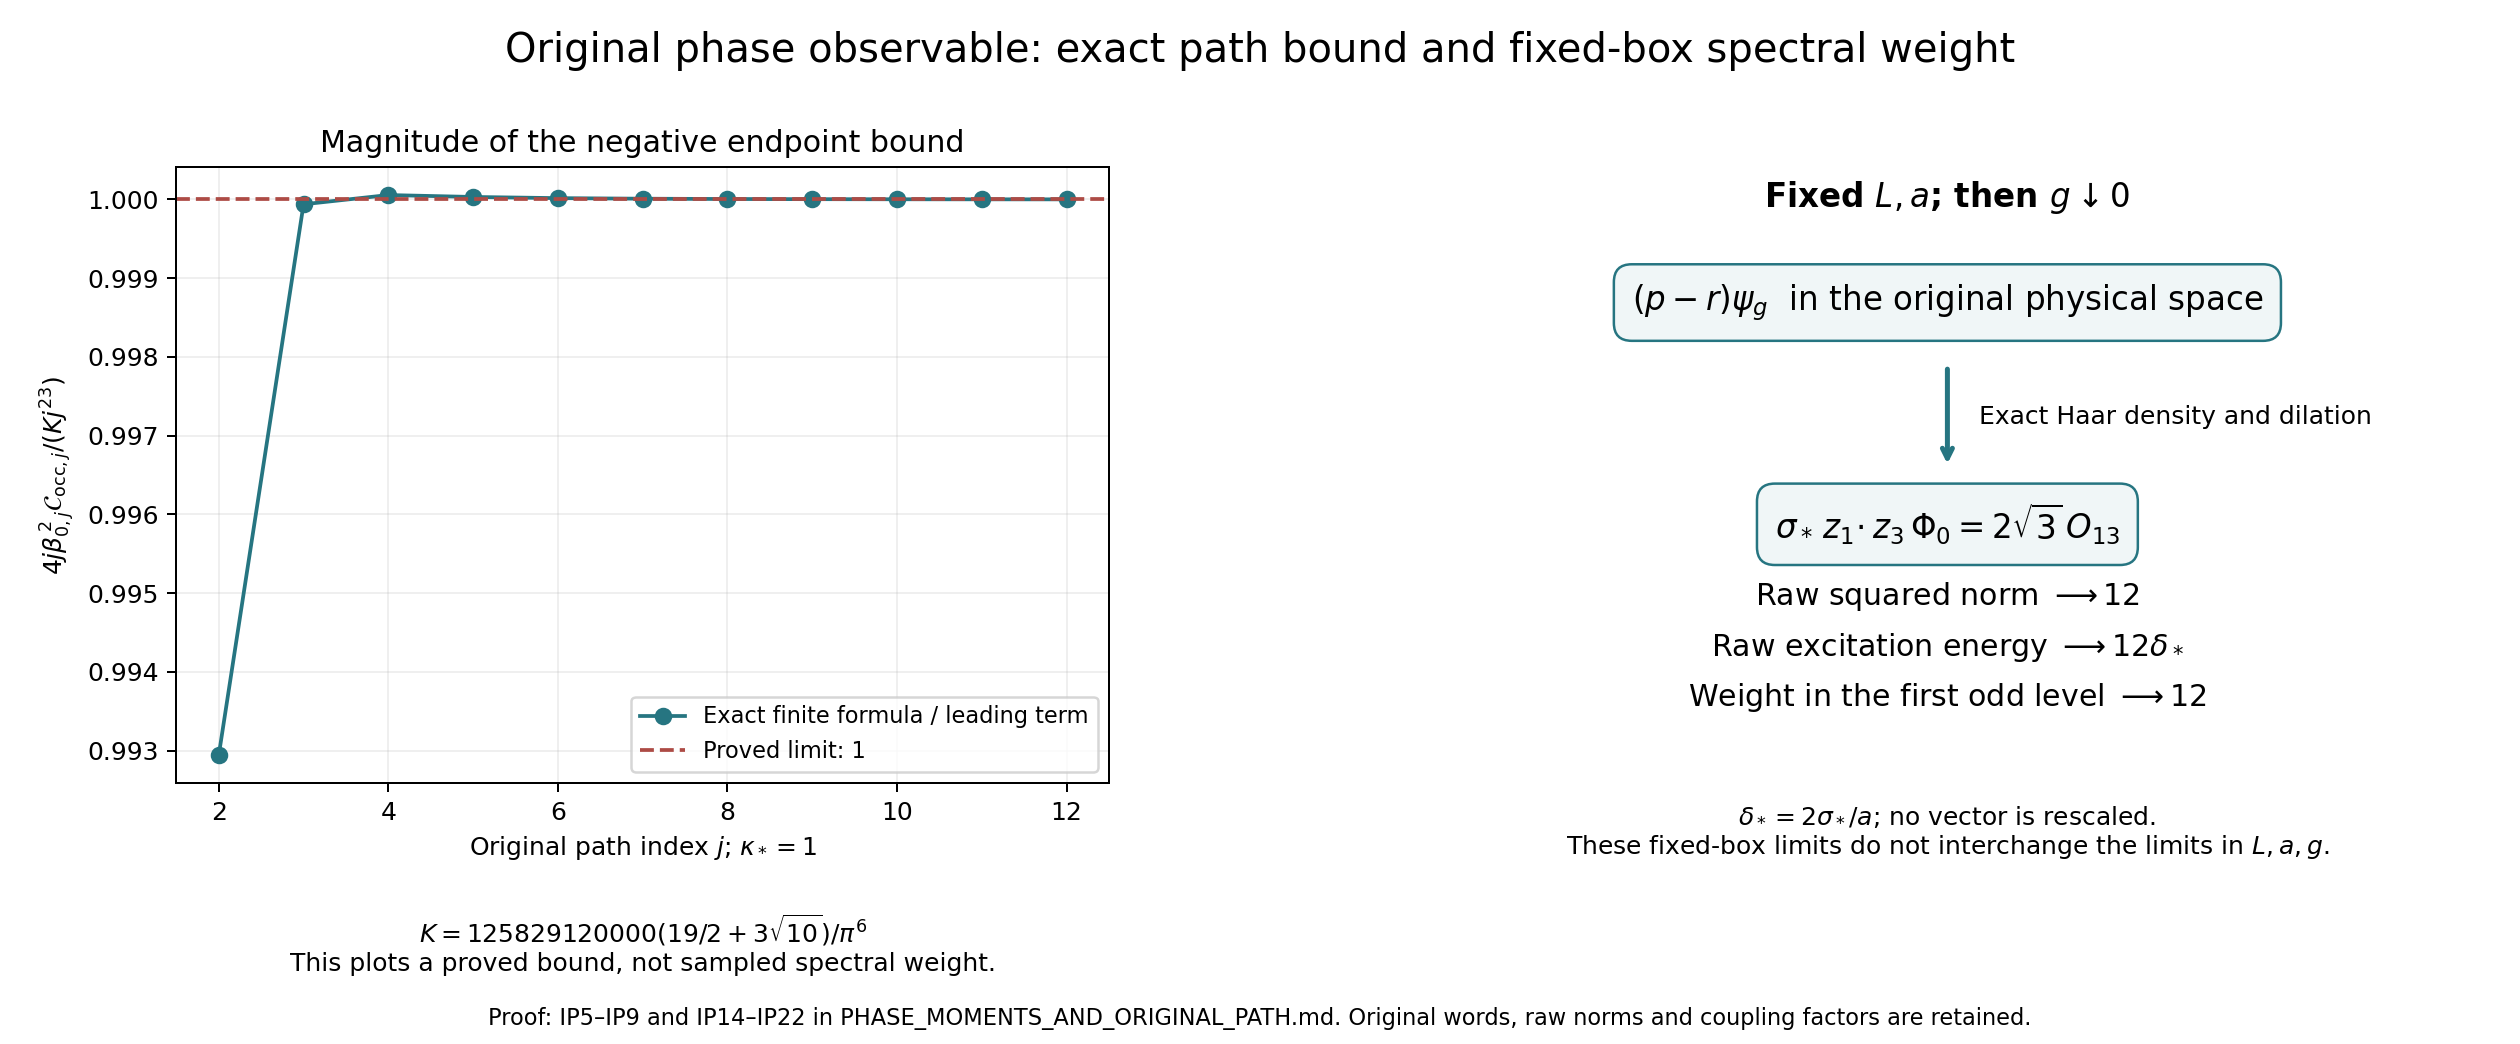
\includegraphics[width=\linewidth,height=.72\textheight,keepaspectratio]{PHASE_MOMENTS_AND_ORIGINAL_PATH.png}\caption{Exact original-path occurrence bound and fixed-box spectral receiving map}\end{figure}

The left panel evaluates the finite bound in IP8 divided by its full leading coefficient in IP9. The right panel shows the exact density-and-dilation receiving map and the raw limits in IP18–IP19. The order of limits is fixed-box throughout that panel. Reproducible source: phase\_moments\_figure.py.
\clearpage
\section*{The original center-sign involution, all odd Schur coefficients, and a complete even tail}

11 October 2026. Independent derivation for the original open three-dimensional box. The Hamiltonian, its scalar, link orientations, all vertex constraints, product-spin blocks and union labels are retained.

The center-change mechanism has a human antecedent: L. Li and Y. Meurice, \href{https://arxiv.org/abs/hep-lat/0410029v2}{*Lattice gluodynamics at negative \(g^2\)*, arXiv:hep-lat/0410029v2}, \href{https://arxiv.org/src/hep-lat/0410029v2}{original author TeX}, Section IV, source lines 301–353, especially the labelled equations eq:su2id and eq:parity. They prove a negative-coupling identity for the Wilson action on even periodic lattices and perturbative parity consequences. Below the exact map is proved on the programme's open-box Hamiltonian and labelled Jacobian source. No novelty claim is made for the center-sign mechanism.

The original programme inputs have verified pinned sources: \href{https://github.com/KokunoYumeto/yang-mills-interacting-workbench/blob/fa79faff2cd697e16cfa3a7953f36810c22c8922/yang-mills/continuations/20260915-gauge-native-band/RESEARCH_NOTE.md}{G1–G31, original objects and labelled bilinear bound}; \href{https://github.com/KokunoYumeto/yang-mills-interacting-workbench/blob/33a4c39de32c2c7fdf6f8ce796e40389f766669f/yang-mills/consolidation/20260921-fifth-reference/package/workbench/yang-mills/continuations/20260921-fifth-reference-return/FIFTH_REFERENCE.md}{F1–F42, the full fifth reference}, especially F10 at source line 98, F26 at 272 and F31 at 319; and \href{https://github.com/KokunoYumeto/yang-mills-interacting-workbench/blob/fa79faff2cd697e16cfa3a7953f36810c22c8922/yang-mills/continuations/20260915-gauge-native-band/BAND_AND_CERTIFICATE.md#L125}{B13–B16, every original two-face channel}. The earlier J1–J7 second-coefficient calculation is reproduced as P27–P30 below. The full \href{https://github.com/KokunoYumeto/yang-mills-interacting-workbench/blob/main/yang-mills/continuations/20261011-central-signs-shrinking-window/BASELINE_J5.md}{original provider}, including its outgoing Gram calculation, is also retained.

\subsection*{P1. Original objects and domains}

Let \(L\ge2\) be an integer,
\[
 V_L=\{-L,\ldots,L\}^3,\qquad
 E_L=\{(n,i):n,n+e_i\in V_L,\ 1\le i\le3\}.
\]
The original configuration space is \(SU(2)^{E_L}\) with product Haar probability \(dU\). Every positive edge \(e=(n,i)\) carries \(U_i(n)\). The physical Hilbert space is the invariant part of this Haar \(L^2\) under every vertex gauge transformation, including boundary vertices. The contained faces are \(p=(n;i,j)\), \(i<j\), and
\[
 M=3(2L)^2(2L+1)=12L^2(2L+1).
\]
Keep the original oriented words and generator convention:
\[
 W_p(U)=\operatorname{Tr}\{U_i(n)U_j(n+e_i)
 U_i(n+e_j)^{-1}U_j(n)^{-1}\},\quad S=\sum_pW_p,
\]
\[
 T_a=-i\sigma_a/2,\quad
 X_{e,a}f(U)=\left.\frac{d}{dt}f(\ldots,e^{tT_a}U_e,\ldots)\right|_{t=0},
 \quad K=-\sum_{e,a}X_{e,a}^2,
 \quad\Gamma(f,h)=\sum_{e,a}(X_{e,a}f)(X_{e,a}h).
 \tag{P1}
\]
The original Hamiltonian remains
\[
 H_L(\xi)=\kappa K+\kappa\xi(2M-S),\qquad
 \kappa=2g^2/a,\quad\xi=1/(4g^4),\quad a,g>0. \tag{P2}
\]
For the comparison \(\xi\leftrightarrow-\xi\), fix the actual positive value of \(\kappa\) and extend only the coefficient \(\xi\) to real or complex values. This does not assign negative \(\xi\) to the original positive-\(g\) physical path.

The original operator domain is the physical part of \(H^2(SU(2)^{E_L})\), and the form domain is its physical \(H^1\). The potential is bounded and smooth, so these domains are unchanged for every complex \(\xi\). This is an analytic closed-operator family on a fixed domain; for real \(\xi\) it is self-adjoint with compact resolvent. These are the original domains of F1–F3.

\subsection*{P2. Explicit involution, gauge constraints and boundaries}

For every original positive edge define
\[
 a_i(n)=\sum_{k<i}n_k\in\mathbb Z,\quad
 z_i(n)=(-1)^{a_i(n)}I_2,\quad
 (\tau U)_i(n)=z_i(n)U_i(n),\quad
 (Tf)(U)=f(\tau U). \tag{P3}
\]
Negative integer coordinates have their usual parity. Each \(z_i(n)^2=I_2\), so \(\tau^2=I\). Haar invariance in each edge gives \(T^*=T^{-1}=T\) and \(T1=1\).

For \(i<j\), the four center factors in the original oriented face word are
\[
 z_i(n)z_j(n+e_i)z_i(n+e_j)^{-1}z_j(n)^{-1}.
\]
Since \(a_i(n+e_j)=a_i(n)\) and \(a_j(n+e_i)=a_j(n)+1\), their exponent is
\[
 a_i(n)+[a_j(n)+1]-a_i(n)-a_j(n)=1.
\]
Thus the actual face holonomy acquires \(-I_2\), with its order and inverses unchanged:
\[
 TW_p=-W_p,\qquad TS=-S. \tag{P4}
\]
Only the four contained edges were used, so this proves the statement on every boundary face without adding exterior edges.

For an original vertex gauge transformation \(G=(G_v)\),
\[
 (G\cdot U)_i(n)=G_nU_i(n)G_{n+e_i}^{-1}.
\]
Centrality proves \(\tau(G\cdot U)=G\cdot(\tau U)\) at every edge, including boundary endpoints. Hence \(T\) commutes with the full gauge action and gauge averaging and restricts to a unitary involution on the physical Hilbert space.

The same centrality gives \(z_e e^{tT_a}U_e=e^{tT_a}z_eU_e\), so
\[
 X_{e,a}T=TX_{e,a},\quad KT=TK,\quad
 T\Gamma(f,h)=\Gamma(Tf,Th). \tag{P5}
\]
These identities first hold on smooth functions. The smooth measure-preserving map \(\tau\), and its commutation with every original derivative, preserve \(H^1,H^2\) and extend the domain identities. Haar invariance also gives \(TP_H=P_HT=P_H\), where \(P_Hf=\int f\,dU\). Therefore \(T\) commutes with \(Q_H=I-P_H\), every original \(K\)-spectral projection and \(K^{-1}\) on the nonconstant physical blocks.

\subsection*{P3. Every support label and the assembly quotient}

For the original product-spin label \(j=(j_e)\), keep
\[
 c_j=\sum_ej_e(j_e+1),\quad
 \pi_j(U)=\bigotimes_e\pi_{j_e}(U_e),\quad
 A_j(f)=d_j\int f(U)\pi_j(U)^*\,dU.
\]
Since \(\pi_{j_e}(-I_2)=(-1)^{2j_e}I\),
\[
 \chi(j)=\prod_{e=(n,i)}(-1)^{2j_ea_i(n)}\in\{1,-1\},\quad
 \pi_j(\tau U)=\chi(j)\pi_j(U),\quad
 A_j(Tf)=\chi(j)A_j(f). \tag{P6}
\]
No spin block or active edge is moved.

Write \(\mathscr V_L\) for the completed original physical zero-Haar-mean labelled coefficient space. An entry \(A_{A,j}\) retains its nonempty edge label \(A\supseteq\operatorname{supp}(j)\), including strict containments. Its norm is
\[
 \|f\|_{\rm loc}=\max_{b\in E_L}
 \sum_{A\ni b}\sum_{j\ne0}c_j\|A_{A,j}\|_1. \tag{P7}
\]
Define \(T\) by \(A_{A,j}\mapsto\chi(j)A_{A,j}\). The actual label, matrix dimensions and Casimir remain. This is an isometric involution on the completion.

Assembly has coefficients
\[
 (\operatorname{Asm}A)_j=\sum_{A\supseteq\operatorname{supp}(j)}A_{A,j}.
\]
Its total \(c_j\)-weighted coefficient norm is at most \(|E_L|\|A\|_{\rm loc}\): every nonempty label occurs at least once in the sum over all anchors. Its kernel is therefore the closed subspace
\[
 \mathscr N_L=\left\{A:
 \sum_{A\supseteq\operatorname{supp}(j)}A_{A,j}=0
 \text{ for every }j\right\}. \tag{P8}
\]
The character \(\chi(j)\) does not depend on the enlarged label, so \(T\mathscr N_L=\mathscr N_L\). It induces an isometric involution on the Banach quotient \(\widehat{\mathscr V}_L=\mathscr V_L/\mathscr N_L\), with exact intertwining \(T\operatorname{Asm}=\operatorname{Asm}T\).

Keep the original union-labelled bilinear map
\[
 \mathcal B(f,h)_A=K^{-1}Q_H
 \sum_{A_1\cup A_2=A}\sum_{e,a}
 (X_{e,a}f_{A_1})(X_{e,a}h_{A_2}). \tag{P9}
\]
Equation (P5) proves the label-by-label identity
\[
 T\mathcal B(f,h)=\mathcal B(Tf,Th). \tag{P10}
\]
The removed scalar remains the separately recorded energy scalar and is fixed by \(T\).

Here are the original estimates needed for completion and inversion. A nonzero physical block contains a singlet at every vertex, so \(j_e\le\sum_{f\ne e,\ f\ni v}j_f\). At the endpoints of one edge, the sum \(J_1\) of the other incident spins obeys \(J_1\ge2j_e\). Their outer endpoints are distinct because the cubic graph is simple and triangle-free. The vertex inequalities at those endpoints give \(J_1\le2J_2\), counting each further edge at most twice. Thus \(\sum_fj_f\ge4j_e\). Since \(j(j+1)\ge3j/2\) at every nonzero half-integer,
\[
 c_j\ge6j_e,\qquad \sum_ej_e\le\tfrac23c_j. \tag{P11}
\]
The full original coefficient product obeys \(\|fh\|_X\le\|f\|_X\|h\|_X\): unitarily decompose the tensor-product representation with all multiplicities, pinch to irreducible blocks, and partially trace their multiplicity spaces. Pinching contracts trace norm; the partial trace contracts it by duality against \(Z\otimes I\), \(\|Z\|\le1\). The original spin generator has norm \(j_e\), yielding the derivative bound \(j_e\|A_j\|_1\). Define the unchanged F6 norms
\[
 m(f)=\max_b\sum_{A\ni b,j}\Big(\sum_ej_e\Big)\|A_{A,j}\|_1,\qquad
 t(f)=\max_e\sum_{A\ni e,j}j_e\|A_{A,j}\|_1.
\]
An output anchor belongs to at least one input union label. Sum first over anchors in the first input and then those in the second. The possible double counting only increases the nonnegative bound. The three generators give factor 3, while the actual output Casimir cancels its inverse in (P9). Therefore
\[
 \|\mathcal B(f,h)\|_{\rm loc}
 \le3\{m(f)t(h)+m(h)t(f)\}
 \le\tfrac23\|f\|_{\rm loc}\|h\|_{\rm loc}. \tag{P12}
\]
The last inequality uses \(m(f)\le2\|f\|_{\rm loc}/3\) and \(t(f)\le\|f\|_{\rm loc}/6\), proved by (P11). In particular,
\[
 \|2\mathcal B(q,\cdot)\|\le m(q)+4t(q). \tag{P13}
\]
The bounds include every boundary anchor and are independent of \(L\).

Assembly of (P9) is \(K^{-1}Q_H\Gamma(\operatorname{Asm}f,\operatorname{Asm}h)\). This follows first for finite coefficients, then by continuity: at fixed finite \(L\), the total \(c_j\)-weighted norm controls every first and second derivative, since \(j_e\le c_j\), \(j_e^2\le c_j\), and \(j_ej_f\le[j_e(j_e+1)+j_f(j_f+1)]/2\le c_j\). Thus \(\mathcal B(\mathscr N_L,\mathscr V_L)\) and \(\mathcal B(\mathscr V_L,\mathscr N_L)\) lie in \(\mathscr N_L\). Equations (P10)–(P13) descend to the quotient by taking infima over representatives.

\subsection*{P4. Original face space and coefficient parity}

Let \(P\) be the original physical spectral projection onto \(\ker(K-3)\), acting blockwise while retaining every label \(A\), and \(R=I-P\). These projections contract (P7), preserve (P8), and commute with \(T\).

The exact face-space identification follows in the original blocks. If \(c_j=3\), there are at most four active edges, because each contributes at least \(3/4\). The singlet inequalities exclude valence-one active vertices. Such a finite graph contains a cycle. The cubic graph has no triangle or odd cycle, so all four edges form one elementary face and there are no others. The singlet at each two-edge vertex forces equal spins, and \(4j(j+1)=3\) forces \(j=1/2\). Each such vertex invariant is one-dimensional; contracting the four original indices gives \(W_p\). Conversely \(W_p\) is physical and \(KW_p=3W_p\). Distinct faces have distinct product-spin supports and are orthogonal; successive Haar integration gives \(\int W_p^2\,dU=1\). This proves the G8 identity and, by (P4),
\[
 \ker(K-3)=\operatorname{span}\{W_p\},\qquad TP=PT=-P. \tag{P14}
\]
An enlarged label does not change its spin character.

Retain the complete original recurrence
\[
 v_1=S/3,\qquad v_n=\sum_{i=1}^{n-1}\mathcal B(v_i,v_{n-i})\quad(n\ge2).
 \tag{P15}
\]
The base case is \(Tv_1=-v_1\). If \(Tv_i=(-1)^iv_i\) for all \(i<n\), then (P10) gives
\[
 Tv_n=\sum_{i=1}^{n-1}\mathcal B((-1)^iv_i,(-1)^{n-i}v_{n-i})
 =(-1)^nv_n.
\]
Hence, on the original labelled source,
\[
 \boxed{Tv_n=(-1)^nv_n\quad(n\ge1).} \tag{P16}
\]
In particular an actual coefficient at \((A,j)\) is zero when \(\chi(j)\ne(-1)^n\); the recurrence and every original label remain intact.

For the fifth reference define
\[
 q_5(\xi)=\sum_{i=1}^5\xi^iv_i,\quad
 J_i=2\mathcal B(v_i,\cdot),\quad
 J_5(\xi)=\sum_{i=1}^5\xi^iJ_i.
\]
Here \(J_i\) denotes the coefficient called \(J_{[i]}\) in the earlier J1–J7, whereas \(J_5(\xi)\) denotes the fifth-reference polynomial. Equations (P10),(P16) imply
\[
 Tq_5(\xi)=q_5(-\xi),\quad TJ_iT=(-1)^iJ_i,\quad
 TJ_5(\xi)T=J_5(-\xi). \tag{P17}
\]

\subsection*{P5. Certified analytic disk and full complementary inverse}

The original F26 supplies proved upward bounds \(m(v_i)\le m_i\), \(t(v_i)\le t_i\):
\[
\begin{array}{c|cc}
i&m_i&t_i\\\hline
1&64/3&16/3\\
2&5834/39&137/6\\
3&336572872/208845&225985217/1253070\\
4&17270702970768271/341697152160&110695177857394584026401/18025447358750832000\\
5&1638684&190128 .
\end{array}\tag{P18}
\]
They concern the full original coefficients, including all source rows and boundary anchors. This derivation reads the proofs and receiving estimates; it does not claim a fresh replay of the inherited 662-representative catalogue. Their exact source versions and hashes are in `SOURCE\_READING\_USE\_LEDGER.json`.

By (P13), \(\|J_i\|\le a_i=m_i+4t_i\), explicitly
\[
\begin{split}
a_1&=128/3,\quad a_2=3132/13,\quad a_3=292337810/125307,\\
a_4&=169232115504453213210913/2253180919843854000,\quad
a_5=2399196.
\end{split}\tag{P19}
\]
Put \(\ell(x)=\sum_{i=1}^5a_ix^i\) and let \(\beta\) be the unique positive root of \(\ell(\beta)=1\). All \(a_i>0\), so \(\ell\) is strictly increasing on \([0,\infty)\), starts at zero and tends to infinity, proving existence and uniqueness. Exact rational bisection is retained in `EXACT\_CHECKS.json`; \(\beta\approx0.020200392941788888\) is only a display value.

For every complex \(\xi\) with \(x=|\xi|<\beta\),
\[
 \|J_5(\xi)\|\le\ell(x)<1.
\]
Since \(R\) contracts, on the full original complement of either the labelled source or its quotient,
\[
 D_5(\xi)=R-RJ_5(\xi)R,\qquad
 \boxed{D_5(\xi)^{-1}=\sum_{k=0}^\infty(RJ_5(\xi)R)^k,\quad
 \|D_5(\xi)^{-1}\|\le\frac1{1-\ell(x)}.} \tag{P20}
\]
The constant term is the identity \(R\) of that complementary space. The tail after \(k=N\) is bounded by \(\ell(x)^{N+1}/(1-\ell(x))\). Convergence is uniform on each compact subdisk, proving operator holomorphy on the full certified disk \(D_\beta\). No maximal-radius claim is made.

Exact rational evaluation gives
\[
 \ell(19/1000)<93/100,\qquad
 \|D_5(\xi)^{-1}\|<100/7\quad(|\xi|\le19/1000). \tag{P21}
\]
Thus this bound covers the entire original fifth-source interval \(x\le\alpha\), since F29 gives
\[
 0.018424953576117616681<\alpha
 <0.018424953576117616682<19/1000 .
\]
This estimates the full complementary operator, not a face compression. From (P17),
\[
 TD_5(\xi)T=D_5(-\xi),\qquad
 TD_5(\xi)^{-1}T=D_5(-\xi)^{-1}. \tag{P22}
\]
The same relations hold coefficientwise as formal series.

\subsection*{P6. Every odd Schur coefficient vanishes before assembly}

The original Schur map is
\[
 \mathscr S_5(\xi)=P-PJ_5(\xi)P
 -PJ_5(\xi)R D_5(\xi)^{-1}RJ_5(\xi)P. \tag{P23}
\]
It is a bounded holomorphic face-range map on \(D_\beta\). Equations (P17),(P22) give \(T\mathscr S_5(\xi)T=\mathscr S_5(-\xi)\). By (P14), both its endpoint actions of \(T\) are \(-I\). Therefore
\[
 \boxed{\mathscr S_5(-\xi)=\mathscr S_5(\xi).} \tag{P24}
\]

More strongly, for \(k\ge1\) and \(i_s\in\{1,\ldots,5\}\), define the literal word
\[
 F_{i_1,\ldots,i_k}=PJ_{i_1}RJ_{i_2}R\cdots RJ_{i_k}P,
 \quad F_i=PJ_iP\text{ if }k=1.
\]
Conjugating each factor gives
\[
 TF_{i_1,\ldots,i_k}T=(-1)^{i_1+\cdots+i_k}F_{i_1,\ldots,i_k},
\]
whereas its endpoints and (P14) give \(TF_{i_1,\ldots,i_k}T=F_{i_1,\ldots,i_k}\). Consequently
\[
 \boxed{F_{i_1,\ldots,i_k}=0
 \quad\text{whenever }i_1+\cdots+i_k\text{ is odd}.} \tag{P25}
\]
This is a labelled-source identity, for every original union label, and therefore descends to the quotient. No cancellation between different words is required.

In particular the full third coefficient is
\[
 [\xi^3]\mathscr S_5
 =-PJ_3P-PJ_1RJ_2P-PJ_2RJ_1P-PJ_1RJ_1RJ_1P=0. \tag{P26}
\]
Each of these four summands is zero separately. Every \([\xi^{2r+1}]\mathscr S_5\), \(r\ge0\), vanishes; no higher even channel is discarded.

\subsection*{P7. The retained complete second coefficient}

To combine the original J1–J6 with this result, keep all their intermediate channels. Put \(D_p=\chi_1(U_p)\). From \(W_p^2=1+D_p\),
\[
 KD_p=8D_p,\quad\|D_p\|_H^2=1,\quad
 \Gamma(W_p,W_p)=3-D_p.
\]
For adjacent faces \(p\sim q\), let \(C_{0,pq},C_{1,pq}\) be the original shared-edge spin-zero and spin-one projections of \(W_pW_q\). Cyclic trace and inversion of a whole SU(2) trace put the ordered words at that edge into \(\operatorname{Tr}(UA),\operatorname{Tr}(U^{-1}B)\), retaining the two three-link paths. The six nonshared links are independent Haar factors; successive integration makes \(A,B\) independent Haar variables, also independent of \(U\). Thus \(\|W_pW_q\|_H^2=1\), while \(\|\operatorname{Tr}(AB)/2\|_H^2=1/4\). Orthogonality of the two shared-edge spin projections gives the remaining norm \(3/4\). In full,
\[
 C_0=\tfrac12\operatorname{Tr}(AB),\quad C_0+C_1=W_pW_q,\quad
 KC_0=\tfrac92C_0,\quad KC_1=\tfrac{13}2C_1,
\]
\[
 \|C_0\|_H^2=\tfrac14,\quad\|C_1\|_H^2=\tfrac34,\quad
 \langle C_0,C_1\rangle_H=0.
\]
The product rule \(K(fh)=(Kf)h+f(Kh)-2\Gamma(f,h)\) gives
\(\Gamma(W_p,W_q)=3C_0/4-C_1/4\). Nonadjacent derivative supports are disjoint. The self-face scalar 3 is removed only by the original \(Q_H\). Thus the complete outgoing map is
\[
 J_1W_p=-\tfrac1{12}D_p+
 \sum_{q\sim p}\left(\tfrac19C_{0,pq}-\tfrac1{39}C_{1,pq}\right).
 \tag{P27}
\]
Its Casimirs imply \(PJ_1P=0\).

Two different unordered face pairs have different independent link-center characters. Otherwise the mod-two sum of at most four distinct faces would have zero edge boundary. Each of the four edges of an included face would require a different other face, since distinct elementary faces share at most one edge. At least five faces would be required, a contradiction. The pair characters are also distinct from the completely even spin-one face character. Haar substitution therefore gives exactly the pair-selection rules below.

For a Casimir-\(c\) component \(h_c\), integration by parts and the product rule give
\[
 \Gamma(S,\cdot)^*=3S-\Gamma(S,\cdot),\quad
 \langle h_c,\Gamma(S,W_r)\rangle_H
 =\tfrac{6-c}{2}\langle h_c,SW_r\rangle_H .
\]
Keeping \(PK^{-1}Q_H=P/3\) yields
\[
 PJ_1h_c=\tfrac c9PSh_c. \tag{P28}
\]
Indeed its scalar factor is \((2/9)[3-(6-c)/2]=c/9\).
The selection rules force the two fundamental face factors in \(PSD_p\) to coincide. If their common face is \(r\ne p\), then \(\int W_r^2D_p=\int(1+D_r)D_p=0\) by the distinct spin-one supports. The surviving integral is \(\int W_p^2D_p=1\), giving \(PSD_p=W_p\). For the two shared-edge channels only the original unordered pair survives, and its face integrals are exactly their squared Haar norms. Hence
\[
 PJ_1D_p=\tfrac89W_p,\quad
 PJ_1C_0=\tfrac18(W_p+W_q),\quad
 PJ_1C_1=\tfrac{13}{24}(W_p+W_q).
\]
The adjacent return keeps the two terms
\[
 \tfrac19\tfrac18(W_p+W_q)
 -\tfrac1{39}\tfrac{13}{24}(W_p+W_q)
 =(\tfrac1{72}-\tfrac1{72})(W_p+W_q)=0.
\]
The self-face return is \(-\tfrac1{12}\tfrac89W_p=-2W_p/27\). Therefore
\[
 PJ_1RJ_1P=PJ_1^2P=-\tfrac2{27}P. \tag{P29}
\]

The complete second source is
\[
 v_2=-\tfrac1{72}\sum_pD_p+
 \sum_{\{p,q\}:p\sim q}
 \left(\tfrac1{27}C_{0,pq}-\tfrac1{117}C_{1,pq}\right).
\]
For a Casimir-\(c\) part \(f_c\), projecting the product rule gives
\(P\Gamma(f_c,W_q)=cP(f_cW_q)/2\); its contribution to \(PJ_2W_q\) is \(cP(f_cW_q)/3\). The self coefficient is
\(-\tfrac1{72}\tfrac83=-1/27\). The two adjacent coefficients to either face are
\[
 \tfrac1{27}\frac{9/2}{3}\tfrac14=\tfrac1{72},\qquad
 -\tfrac1{117}\frac{13/2}{3}\tfrac34=-\tfrac1{72}.
\]
Thus, preserving both contributions,
\[
 PJ_2P=-\tfrac1{27}P,\qquad
 -PJ_2P-PJ_1RJ_1P=\tfrac19P. \tag{P30}
\]
For an input face carrying an enlarged label \(A_0\), the self-return label is \(A_0\), and the two cancelling adjacent contributions both have label \(A_0\cup\partial p\cup\partial q\). Hence these identities hold on the entire labelled face range, before quotienting.

\subsection*{P8. A rational bound for the complete remaining even tail}

The Neumann series makes the original Schur expression exactly
\[
 \mathscr S_5(\xi)=P-
 \sum_{k\ge1}\sum_{1\le i_1,\ldots,i_k\le5}
 \xi^{i_1+\cdots+i_k}F_{i_1,\ldots,i_k}. \tag{P31}
\]
For \(x=|\xi|<\beta\), the sum of the operator norms is bounded by
\[
 h(x)=\sum_{k\ge1}\ell(x)^k=\frac{\ell(x)}{1-\ell(x)}.
\]
Thus regrouping by total degree is valid. Write \(h(x)=\sum_{n\ge1}h_nx^n\); all \(h_n\ge0\), and
\(\|[\xi^n](P-\mathscr S_5)\|\le h_n\). In particular
\[
 h_2=a_2+a_1^2=\frac{241180}{117}. \tag{P32}
\]
Put \(e(x)=a_2x^2+a_4x^4\), \(o(x)=a_1x+a_3x^3+a_5x^5\). The full even part is
\[
 \frac{h(x)+h(-x)}2
 =\frac12\left\{\frac{e+o}{1-e-o}+\frac{e-o}{1-e+o}\right\}
 =\frac{e-e^2+o^2}{(1-e)^2-o^2}. \tag{P33}
\]
For \(x<\beta\), both denominator factors \(1-e-o\) and \(1-e+o\) are positive. Retain the entire numerator and denominator and define
\[
 \mathcal E_4(x)=
 \frac{e(x)-e(x)^2+o(x)^2}{[1-e(x)]^2-o(x)^2}
 -(a_2+a_1^2)x^2
 =\sum_{r\ge2}h_{2r}x^{2r}. \tag{P34}
\]
Its nonnegative series proves nonnegativity, monotonicity and order four. Combining (P25),(P30),
\[
 \boxed{\mathscr S_5(\xi)=
 (1+\xi^2/9)P+\mathcal R_4(\xi),\quad
 \mathcal R_4(-\xi)=\mathcal R_4(\xi),\quad
 \|\mathcal R_4(\xi)\|\le\mathcal E_4(|\xi|).} \tag{P35}
\]
Every even order at least four and every complementary spin and union label is included. The bound is independent of \(L\) in the original local source norm and the assembly quotient norm.

Exact rational evaluation in `EXACT\_CHECKS.json` proves
\[
 \mathcal E_4(1/100)<66/1000,\qquad
 \mathcal E_4(1/64)<3/4. \tag{P36}
\]
For size only, the corresponding decimals are \(0.06577819999898235\) and \(0.737650994481419\). Since \(x^{2k}\le(x/r)^4r^{2k}\) for \(k\ge2\), \(0\le x\le r<\beta\),
\[
 \mathcal E_4(x)\le(x/r)^4\mathcal E_4(r). \tag{P37}
\]
In particular the entire remainder has bound \((66/1000)(100|\xi|)^4\) on \(|\xi|\le1/100\).

The full \(I-J_5(\xi)\) also has its complete Neumann inverse on \(D_\beta\). Solving its two block equations gives
\[
 \mathscr S_5(\xi)^{-1}=P(I-J_5(\xi))^{-1}P,\qquad
 \|\mathscr S_5(\xi)^{-1}\|\le\frac1{1-\ell(|\xi|)}. \tag{P38}
\]
For a face forcing \(f\), the complementary equation gives \(u_R=D_5^{-1}RJ_5Pu_P\). Substituting it into the face equation gives exactly (P23); conversely this substitution solves both equations. This proves the block identity and its inverse, including points where (P34) is too large for a small-perturbation estimate.

One further direct consequence of (P36), on the complete complex disk \(|\xi|\le1/64\), is
\[
 |1+\xi^2/9|\ge1-1/36864,\quad
 \|\mathscr S_5(\xi)^{-1}\|<
 \frac1{1-1/36864-3/4}.
\]
No Haar self-adjointness, Schur positivity, new physical gap or enlarged nonlinear source endpoint is inferred from these auxiliary Banach bounds.

\subsection*{P9. Full Hamiltonian and retained vacuum scalar}

Equations (P4),(P5) prove, on the original fixed domain and for every complex \(\xi\),
\[
 \boxed{TH_L(\xi)T
 =\kappa K+\kappa\xi(2M+S)
 =H_L(-\xi)+4\kappa M\xi I.} \tag{P39}
\]
The scalar is the difference of the two original \(2\kappa M\xi\) terms; neither Hamiltonian has lost its scalar.

For real \(\xi\), list the physical eigenvalues in increasing order with multiplicity. Unitary conjugation gives for every \(n\ge0\)
\[
 \boxed{E_{n,L}(\xi)=E_{n,L}(-\xi)+4\kappa M\xi.} \tag{P40}
\]
Subtracting the exact original ground energies consequently yields
\[
 E_{n,L}(\xi)-E_{0,L}(\xi)
 =E_{n,L}(-\xi)-E_{0,L}(-\xi),
\]
\[
 T[H_L(\xi)-E_{0,L}(\xi)]T=H_L(-\xi)-E_{0,L}(-\xi). \tag{P41}
\]
Thus the physical gap on every original finite box is even in the auxiliary real coefficient \(\xi\) at fixed \(\kappa\).

The positive unit ground vector exists and is unique for every real \(\xi\). The original argument F3 applies: compactness supplies a ground minimizer; the derivative modulus inequality makes it nonnegative; elliptic regularity and the strong maximum principle make it smooth and strictly positive. For this vector \(\psi\), integration by parts in its exact eigen-equation gives
\[
 q_{H-E_0}(\psi f)=
 \kappa\int\psi^2\sum_{e,a}|X_{e,a}f|^2\,dU.
\]
Division by the smooth positive \(\psi\) preserves \(H^1\). The quotient of any other ground vector by \(\psi\) has every derivative zero, hence is constant on the connected configuration space. Positivity and unit norm fix that constant. Gauge transformations preserve all these conditions, so uniqueness makes the scalar-space ground vector physical.

Define the original vacuum density \(\rho_L(\xi)=\psi_L(\xi)^2\). Since \(T\) preserves positivity and norm, (P39) and uniqueness give
\[
 \psi_L(-\xi)=T\psi_L(\xi),\qquad
 \rho_L(-\xi)=T\rho_L(\xi). \tag{P42}
\]
The exact zero-Haar logarithm
\[
 v_L(\xi)=\log\psi_L(\xi)-P_H\log\psi_L(\xi)
\]
satisfies \(v_L(-\xi)=Tv_L(\xi)\). The original normalization constant and scalar are
\[
 c_L(\xi)=-\tfrac12\log\int e^{2v_L(\xi)}\,dU,\quad
 C_L(\xi)=P_H\Gamma(v_L(\xi),v_L(\xi)).
\]
Haar invariance and (P5) prove \(c_L(-\xi)=c_L(\xi)\), \(C_L(-\xi)=C_L(\xi)\), with
\[
 E_{0,L}(\xi)=2\kappa M\xi-\kappa C_L(\xi). \tag{P43}
\]
Every original removed scalar is present in this energy equation.

The original multiplication map \(\mathcal U_\xi f=\psi_L(\xi)f\) from \(L^2(\rho_L(\xi)dU)\) to Haar \(L^2\) has the exact intertwining
\[
 \mathcal U_{-\xi}T=T\mathcal U_\xi.
\]
Here \(T:L^2(\rho_L(\xi)dU)\to L^2(\rho_L(-\xi)dU)\) is unitary by Haar substitution. Combining with (P41) proves covariance of the original ground-transformed operators and their forms. For each integrable observable \(f\),
\[
 \int\rho_L(-\xi)f\,dU=\int\rho_L(\xi)Tf\,dU.
\]
Each original face expectation is therefore odd. This uses the exact different interacting measures and does not replace them by Haar measure.

\subsection*{P10. The complete nonlinear source and its interior inverse}

The parity extends to the full fifth-reference correction by its proved construction. Retain
\[
 R_5(\xi)=\xi v_1+\mathcal B(q_5(\xi),q_5(\xi))-q_5(\xi),\qquad
 L_5(\xi)=I-J_5(\xi).
\]
Equations (P10),(P17) give \(TR_5(\xi)=R_5(-\xi)\) and \(TL_5(\xi)^{-1}T=L_5(-\xi)^{-1}\) on \(D_\beta\). For the complete original tree series,
\[
 w_1=L_5^{-1}R_5,\qquad
 w_n=L_5^{-1}\sum_{i+j=n}\mathcal B(w_i,w_j),
\]
induction gives \(Tw_n(\xi)=w_n(-\xi)\). Its proved F30–F32 absolute convergence on \(|\xi|\le\alpha\) gives
\[
 T[q_5(\xi)+\sum_{n\ge1}w_n(\xi)]
 =q_5(-\xi)+\sum_{n\ge1}w_n(-\xi). \tag{P44}
\]
Absolute convergence includes the closed boundary. On the real interval, the original positive-ground reconstruction identifies this source with the logarithm in (P43).

Retain every scalar in
\[
 b_{ij}=3(m_it_j+m_jt_i),\quad
 \delta(x)=\sum_{1\le i,j\le5,\ i+j\ge6}b_{ij}x^{i+j},
\]
\[
 \mathscr D(x)=[1-\ell(x)]^2-\tfrac83\delta(x),\qquad
 w_*(x)=\tfrac34[1-\ell(x)-\sqrt{\mathscr D(x)}].
\]
Original F31 proves \(\|v-q_5\|\le w_*(x)\), and \(\mathscr D(x)>0\) for \(0\le x<\alpha\). For the actual full Jacobian \(J(\xi)=2\mathcal B(v(\xi),\cdot)\), (P12) therefore gives
\[
 \|J(\xi)\|\le\ell(x)+\tfrac43w_*(x)
 =1-\sqrt{\mathscr D(x)}<1.
\]
Consequently the full nonlinear complementary inverse exists on that interior disk and
\[
 \boxed{\|(R-RJ(\xi)R)^{-1}\|
 \le1/\sqrt{\mathscr D(x)}\quad(0\le x<\alpha).} \tag{P45}
\]
Its Schur map is even by the same conjugation proof. At \(x=\alpha\), this estimate has zero denominator and asserts no endpoint inverse. The polynomial-reference inverse (P20) remains finite there. Their exact connecting perturbation is
\[
 J-J_5=2\mathcal B(v-q_5,\cdot),\qquad
 \|J-J_5\|\le\tfrac43w_*.
\]

\subsection*{P11. Exact human-source comparison and receiving calculation}

Li–Meurice's Section II, original source lines 162–198, uses the \(SU(2)\) action
\(\beta_{\rm LM}\sum_p(1-W_p/2)\) on symmetric periodic lattices with even side length. Here \(\beta_{\rm LM}\) denotes their original variable \(\beta\), distinguished from the inverse-radius root in P5. The original potential here is exactly
\[
 \kappa\xi\sum_p(2-W_p)=2\kappa\xi\sum_p(1-W_p/2).
\]
For a static weight \(e^{-tV}\), the full parameter map is \(\beta_{\rm LM}=2t\kappa\xi\); their scalar \(2\beta_{\rm LM}M\) becomes \(4t\kappa M\xi\). The explicit open-box assignment (P3) proves the local action identity on the present geometry, and commutation with every original derivative proves the additional kinetic-operator relation (P39). Thus the quantum heat traces satisfy
\[
 \operatorname{Tr}_{\rm phys}e^{-tH_L(-\xi)}
 =e^{4t\kappa M\xi}\operatorname{Tr}_{\rm phys}e^{-tH_L(\xi)}
 \quad(t>0,\ \xi\in\mathbb R).
\]
This follows by exponentiating (P39) and unitary invariance of trace. For completeness, \(|2M-S|\le4M\), so the min-max principle bounds the full heat trace by
\[
 e^{4t\kappa M|\xi|}
 \left[\sum_{j=0,1/2,\ldots}(2j+1)^2e^{-t\kappa j(j+1)}\right]^{|E_L|}<\infty.
\]
Each one-link sum converges by its Gaussian decay, proving trace class; restriction to the physical reducing subspace preserves it. No equality between the static integral and quantum heat trace is asserted.

Their lines 339–353 explicitly derive perturbative parity and Wilson-loop parity; those results are an antecedent, not a new finding here. Their lines 267–288 discuss gauge equivalence within their constructed collections of special link-line configurations. This note does not use those passages as a classification of all periodic flat central twists.

The previously unfinished J7 calculation is strengthened by (P26), (P20), and (P35): the third coefficient is exactly zero; every higher odd return is zero before assembly; the complete complementary inverse has an explicit uniform bound; and the complete remaining even tail has an explicit rational majorant. The fourth coefficient is now the first unevaluated coefficient that can change this face Schur map. Its value is not replaced by the majorant, and no new nonlinear endpoint or physical gap is inferred. The original fourth return with every spin channel is the next concrete calculation; the full fifth residual and the bounds above supply rigorous remainders while that coefficient is evaluated.
\clearpage
\section*{Central link signs and the exact boundary obstruction}

Multiplying selected \(SU(2)\) links by \(-I\) can reverse every elementary plaquette trace simultaneously. On the original open box this transformation exists and is unique on gauge-invariant functions. On a periodic rectangular box it exists exactly when at most one side has an odd number of links. When it exists there are eight distinct transformations on gauge-invariant functions, distinguished by the signs of the three winding loops. The following construction retains all links, faces, orientations and the full Hamiltonian scalar.

This result supplies the boundary domain of the central-sign symmetry used in the companion Jacobian calculation. It concerns the finite original operator; it does not supply its continuum limit. The original operator conventions are \href{https://github.com/KokunoYumeto/yang-mills-interacting-workbench/blob/485b61423c1f4e1805deb453c1b6b342b27842b6/yang-mills/continuations/20260930-s6-ns-moment-map-bridge/PERIOD_COUPLING_AND_PHYSICAL_KERNELS.md}{PK25 and PK132}. All sign constructions and classification arguments needed here are proved below.

L. Li and Y. Meurice already use center multiplication to reverse plaquette traces on even periodic cubes in \href{https://arxiv.org/abs/hep-lat/0410029v2}{Lattice gluodynamics at negative \(g^2\), arXiv:hep-lat/0410029v2}, Sections II–IV and the Appendix. Their Section III identifies one uniform set of elementary plaquette values and compares particular translated or rotated line constructions. Our classification below concerns all central link assignments and also retains winding traces. The center-reversal mechanism is therefore a literature input; the present proof gives its exact rectangular boundary conditions, winding classes and original Hamiltonian map. No novelty claim is made.

\begin{figure}[htbp]\centering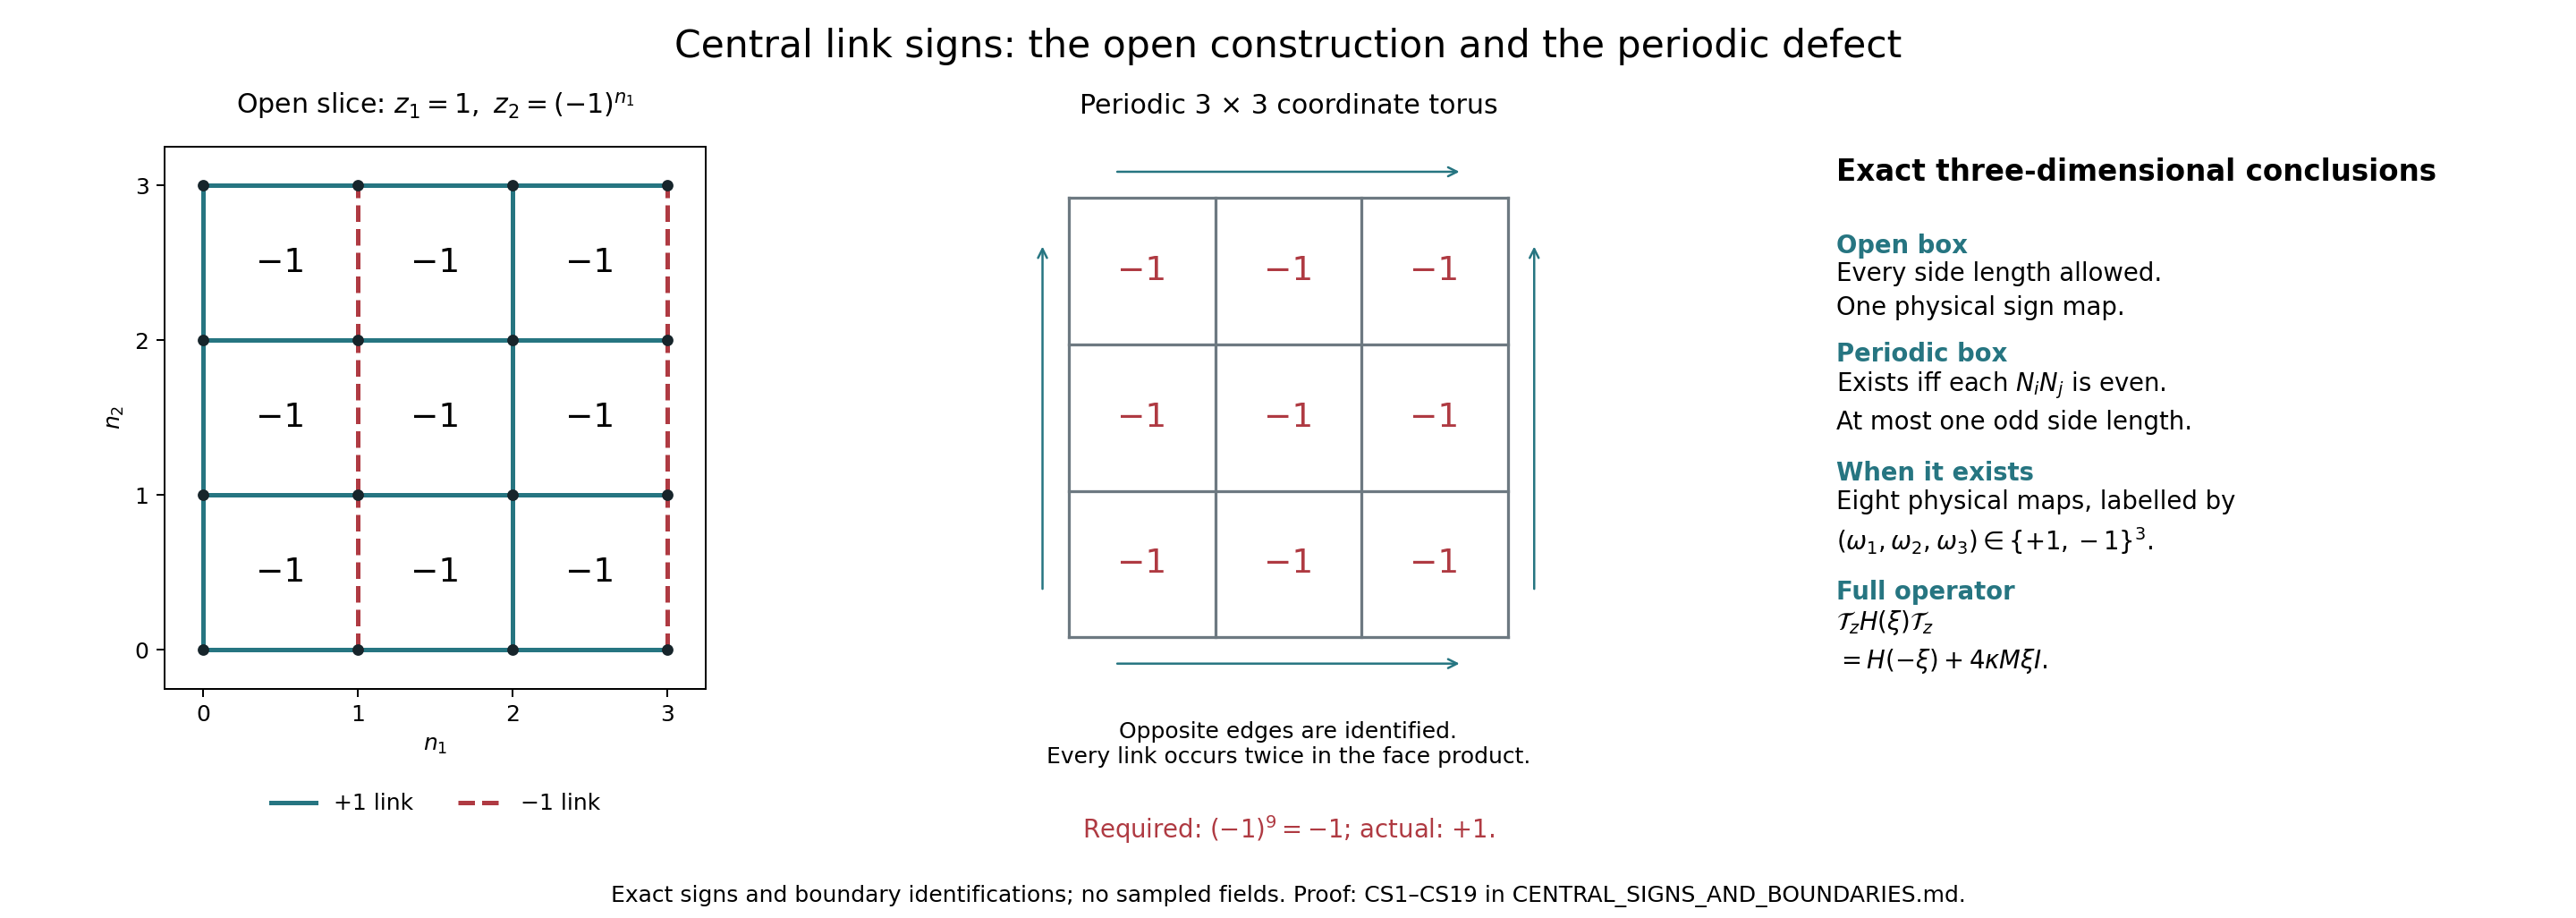
\includegraphics[width=\linewidth,height=.72\textheight,keepaspectratio]{CENTRAL_SIGNS_AND_BOUNDARIES.png}\caption{Exact central link signs and periodic face-product obstruction}\end{figure}

The left panel is an exact coordinate slice of CS6. The middle panel shows the proposed face signs on a periodic \(3\)-by-\(3\) coordinate torus, whose impossibility follows by multiplying all nine faces. The right panel records the complete three-dimensional conclusions proved in CS8–CS19. Figure source: central\_signs\_figure.py.

\subsection*{1. Original link and face maps}

Let the open vertices be
\[
 V_{\rm op}=\prod_{i=1}^3\{0,\ldots,m_i\},\qquad m_i\ge1.
 \tag{CS1}
\]
A positive link \((n;i)\) goes from \(n\) to \(n+e_i\), and is present exactly when \(n_i<m_i\). The face \((n;i,j)\), \(i<j\), is present when both these inequalities hold. Its original ordered holonomy and trace are
\[
 U_{n;ij}=U_i(n)U_j(n+e_i)U_i(n+e_j)^{-1}U_j(n)^{-1},
 \qquad W_{n;ij}=\operatorname{Tr}U_{n;ij}.
 \tag{CS2}
\]
The original cubic box is obtained by \(m_1=m_2=m_3=2L\) and the exact coordinate change \(n=k+(L,L,L)\) from \(k\in\{-L,\ldots,L\}^3\). No physical coordinate, lattice spacing or edge midpoint is changed by this relabelling.

For a central sign assignment \(z_i(n)\in\{1,-1\}\), define
\[
 (D_zU)_i(n)=z_i(n)U_i(n),\qquad
 (\partial z)_{n;ij}
 =z_i(n)z_j(n+e_i)z_i(n+e_j)z_j(n).
 \tag{CS3}
\]
The missing inverse signs in the second formula are intentional: \(z^{-1}=z\). Centrality, without commuting any of the \(U\) factors, gives
\[
 U_{n;ij}(D_zU)=(\partial z)_{n;ij}U_{n;ij}(U).
 \tag{CS4}
\]
For any oriented edge word \(\gamma=(e_1^{\epsilon_1},\ldots,e_q^{\epsilon_q})\), where repetitions and \(\epsilon_l\in\{1,-1\}\) are retained,
\[
 U_\gamma(D_zU)=
       \left(\prod_{l=1}^q z_{e_l}^{\epsilon_l}\right)U_\gamma(U).
 \tag{CS5}
\]
This follows factor by factor from \((zU)^{-1}=z^{-1}U^{-1}\). In particular central signs do not change the order or support of a loop.

\subsection*{2. The open-box construction and its gauge class}

Set, on every existing positive link,
\[
 z_i^0(n)=(-1)^{\,\sum_{k<i}n_k}.
 \tag{CS6}
\]
For \(i<j\), increasing coordinate \(i\) changes \(z_j^0\) by \(-1\), whereas increasing coordinate \(j\) leaves \(z_i^0\) unchanged. Consequently the four factors in CS3 have product \(-1\) on every existing face, including boundary faces. In the original \(k\) coordinates one may instead use \((-1)^{\sum_{h<i}k_h}\). The two assignments differ by direction-dependent constant signs \((-1)^{(i-1)L}\), which have zero face curvature; the argument below proves their physical equivalence.

We prove the complete uniqueness statement. If \(z,z'\) both have face product \(-1\), then \(h_e=z_ez'_e\) has face product \(+1\). Define \(a(n)\) as the product of \(h\) along the monotone root path from \(0\) to \(n\), taking the coordinate directions in the order \(1,2,3\). Set \(a(0)=1\). The equation on an \((i,j)\)-face says exactly that the product along its two monotone two-edge paths is equal. Adjacent exchanges of unlike steps therefore preserve a monotone path product. Every ordering of the same multiset of coordinate steps is obtained by finitely many such adjacent exchanges, and every intermediate path stays inside the box. Appending the edge \((n;i)\) to the chosen path to \(n\), and reordering its steps, gives the chosen path to \(n+e_i\). Thus
\[
 h_i(n)=a(n)a(n+e_i),\qquad
 z'_i(n)=a(n)z_i(n)a(n+e_i).
 \tag{CS7}
\]
Conversely every choice of vertex signs \(a\) in CS7 preserves all face products, because each of the four vertex signs occurs twice. The only assignments \(a\) producing the identity link change are constants: equality of adjacent vertex values and connectedness prove this. There are therefore exactly
\[
 2^{\,|V_{\rm op}|-1}
 \quad\hbox{face-reversing link assignments, and one vertex-sign gauge class.}
 \tag{CS8}
\]
The vertex signs \(a(n)I\) are actual \(SU(2)\) gauge transformations. Hence every face-reversing assignment induces the same transformation on the physical, gauge-invariant Hilbert space.

\subsection*{3. Periodic boxes and the necessary parity condition}

Now take the vertices
\[
 V_{\rm per}=\prod_{i=1}^3\mathbb Z/N_i\mathbb Z,\qquad N_i\ge3.
 \tag{CS9}
\]
Every positive link and every positively based \((i,j)\)-face is retained, including links and faces crossing a periodic seam. The lower bound on \(N_i\) avoids any convention about parallel one-cell or two-cell presentations.

At fixed coordinate in the third direction, multiply \((\partial z)_{n;ij}\) over all \(N_iN_j\) faces of an entire coordinate two-torus. Each of its \(i\)-links occurs in exactly two factors, once at each adjacent \(j\)-position; each \(j\)-link likewise occurs twice. Thus the product is \(+1\) for every \(z\). If every face product were \(-1\), it would instead be \((-1)^{N_iN_j}\). Existence therefore requires
\[
 N_1N_2\equiv N_1N_3\equiv N_2N_3\equiv0\pmod2.
 \tag{CS10}
\]
These three conditions say exactly that at most one \(N_i\) is odd: two odd lengths violate their pair condition, and otherwise each pair contains an even length.

The condition is also sufficient. Choose an ordering \(r_1,r_2,r_3\) of the original coordinate directions with the odd length last if there is one. Each of \(N_{r_1},N_{r_2}\) is then even. For the standard representatives \(0\le n_i<N_i\), set
\[
 z_{r_l}^0(n)=(-1)^{\,\sum_{h<l}n_{r_h}},
       \qquad l=1,2,3.
 \tag{CS11}
\]
Consider a face in directions \(r_h,r_l\), \(h<l\). Its \(r_h\)-links have the same sign at both \(r_l\)-positions. The signs of its \(r_l\)-links differ by \(-1\) at an interior \(r_h\)-step. At a seam step from \(N_{r_h}-1\) to zero, their ratio is \((-1)^{-(N_{r_h}-1)}=-1\), because \(N_{r_h}\) is even. Thus CS3 equals \(-1\) also at every seam. Interchanging the two direction names reverses the oriented face but leaves its central sign \(-1\). The construction preserves the original coordinates and face orientation; the ordering only defines which coordinates occur in the exponent.

\subsection*{4. All periodic assignments and the eight physical maps}

Let \(h\) be any flat periodic assignment, meaning \(\partial h=1\). Define its three winding signs by the original coordinate loops,
\[
 \omega_i(h)=\prod_{q=0}^{N_i-1}h_i(n+qe_i)\in\{1,-1\}.
 \tag{CS12}
\]
This product is independent of the starting coordinate \(n_i\) by cyclic permutation. It is independent of a shift of \(n\) in another direction by multiplying the flat face equations along the intervening full strip; the transverse edges cancel in pairs. Since such shifts connect all bases, CS12 is independent of every base coordinate.

For any \(\omega=(\omega_1,\omega_2,\omega_3)\), define the seam assignment
\[
 k_i^\omega(n)=
 \begin{cases}
 \omega_i,&n_i=N_i-1,\\
 1,&0\le n_i<N_i-1.
 \end{cases}
 \tag{CS13}
\]
It is flat: in each face the two \(i\)-signs are equal and the two \(j\)-signs are equal. Its winding signs are precisely \(\omega_i\).

We next prove, without identifying flatness with triviality, that a flat \(h\) with all three winding signs \(+1\) is a vertex-sign gauge change. Cut the torus at the three seams and use the open box with vertices \(0\le n_i<N_i\) and no seam edges. The open-box proof gives vertex signs \(a(n)\) such that \(h_i(n)=a(n)a(n+e_i)\) on all non-seam edges. For the seam in direction \(i\), fix the other two coordinates and multiply these \(N_i-1\) identities along the coordinate line. The resulting product is \(a(n_i=0)a(n_i=N_i-1)\). Since the complete winding product is \(1\), the missing seam edge has exactly this same sign. CS7 therefore holds on every periodic edge.

For general flat \(h\), the product \(hk^{\omega(h)}\) has trivial winding signs, so the preceding construction applies to it. Consequently the full set of face-reversing assignments, when nonempty, is
\[
 z_i(n)=z_i^0(n)\,k_i^\omega(n)\,a(n)a(n+e_i),
 \quad\omega\in\{1,-1\}^3,\quad a\in\{1,-1\}^{V_{\rm per}}.
 \tag{CS14}
\]
Two choices of \(a\) yield the same link assignment exactly when they differ by one global sign. Different \(\omega\) cannot be related by vertex signs, since vertex signs cancel in a closed-loop product. Thus there are exactly \(2^{|V_{\rm per}|+2}\) assignments and eight vertex-sign gauge classes.

These eight classes induce distinct maps even on physical \(SU(2)\) functions. If two classes differ in winding sign \(i\), apply their transformations to the trace of the winding loop in direction \(i\). By CS5 the two transformed trace functions have opposite signs. This trace is a nonzero continuous gauge-invariant function: at the identity link configuration its value is \(2\). Its nonzero set contains an open set of positive Haar measure. The two Hilbert-space maps therefore differ.

This classification is of central sign assignments. For the larger spaces of \(SU(2)\) fields, CS4 gives the exact additional map: \(D_{z^0}\) sends all configurations with every \(U_p=-I\) bijectively to all flat configurations with every \(U_p=I\), and its own inverse returns them. It commutes with the full vertex gauge group, so the bijection descends to their gauge quotients. The eight central classes above do not assert that these larger quotients have only eight points.

In additive notation \(z_e=(-1)^{t_e}\), the exact defect equation is \(\delta t=\mathbf1_{\rm faces}\) over \(\mathbb F_2\). The constant face assignment is closed, since every cube has six faces. Its three coordinate-torus evaluations are the retained integers \(N_iN_j\) modulo two. The necessity and explicit sufficiency above prove that its obstruction vanishes exactly under CS10; no unspecified cohomological test remains. When it vanishes, its solution space modulo vertex changes is the explicitly constructed eight-element space CS14. On the open box that space has one element.

\subsection*{5. Full Hamiltonian intertwining and path scope}

Let \(\mathcal T_z f=f\circ D_z\) on the original product-Haar Hilbert space. Central multiplication preserves Haar measure, \(D_z^2=I\), and it commutes with every vertex gauge action. Hence \(\mathcal T_z\) is a self-adjoint unitary preserving the physical Hilbert space.

For the original left generators \(X_{e,\alpha}\), centrality gives
\[
 X_{e,\alpha}\mathcal T_z f=\mathcal T_zX_{e,\alpha}f
 \tag{CS15}
\]
on smooth functions, directly by differentiating
\(z_e\exp(tT_\alpha)U_e=\exp(tT_\alpha)z_eU_e\).
The same equality for the closed generators follows by transporting their graph closures; the unitary preserves smooth functions and their inverse images. Thus it preserves the electric form and self-adjoint operator \(K=-\sum_{e,\alpha}X_{e,\alpha}^2\) with their exact domains.

Write
\[
 S=\sum_pW_p,\qquad
 H(\xi)=\kappa K+\kappa\xi(2M-S),\quad \kappa>0,\quad \xi\in\mathbb R.
 \tag{CS16}
\]
Here \(M=\sum_{i<j}m_im_j(m_k+1)\), with \(k\) the remaining direction, on the open rectangular box, and \(M=3N_1N_2N_3\) on the periodic box. For the original open cube this is \(12L^2(2L+1)\). The magnetic multiplication operator is bounded, so the operator domain is that of \(K\) for every real \(\xi\). When the face-reversing assignment exists, CS4 and CS15 prove the full equality
\[
 \mathcal T_zH(\xi)\mathcal T_z
 =\kappa K+\kappa\xi(2M+S)
 =H(-\xi)+4\kappa M\xi I.
 \tag{CS17}
\]
No vacuum scalar is dropped. By unitary equivalence the ordered eigenvalues, with multiplicities on the physical subspace, satisfy
\[
 E_n(\xi)=E_n(-\xi)+4\kappa M\xi.
 \tag{CS18}
\]
Subtracting the \(n=0\) equality from the operator identity gives
\[
 \mathcal T_z[H(\xi)-E_0(\xi)]\mathcal T_z
       =H(-\xi)-E_0(-\xi).
 \tag{CS19}
\]
The complete spectral projections obey the corresponding unitary equality. This is an equality of the original centered operators, not an assertion that individual excited branches must be analytic through a degeneracy.

On the physical positive-coupling path, \(\kappa=2g^2/a\) and \(\xi=1/(4g^4)\). The auxiliary negative \(\xi\) in CS17 holds \(\kappa\) fixed and has no positive real \(g\) with these two same relations. CS17 therefore supplies exact parity of the coefficient problem and an operator comparison, while keeping the original positive-\(g\) regulator path unchanged. It cannot itself decide the shrinking-window four-loop difference or the continuum spectral gap.

\subsection*{6. The next comparison}

The open-box transformation is an exact tool for the existing Jacobian return calculation. On a periodic replacement, CS10 must first be checked; treating an odd-by-odd two-torus as if the same transformation existed would erase the explicit defect proved in Section 3. When CS10 holds, the eight maps CS14 have the same plaquette reversal and full Hamiltonian identity, but their winding-loop actions differ by CS5 and CS12. A continuum comparison involving winding observables must retain which one of those maps is used. The companion calculation uses the original open box and its unique physical map throughout.
\clearpage
Historical source, preserved below. The third coefficient and complete inverse/tail backlog at the end is now resolved by \href{https://github.com/KokunoYumeto/yang-mills-interacting-workbench/blob/main/yang-mills/continuations/20261011-central-signs-shrinking-window/ORIGINAL_J5_PARITY_AND_TAIL.md}{P1–P45}; the fourth coefficient is the next unevaluated term.

\section*{Original first Jacobian block and its exact return}

29 September 2026. This calculation continues the retained fifth-reference residual on the original open cubic box. It uses the complete face channels already proved in \href{https://github.com/KokunoYumeto/yang-mills-interacting-workbench/blob/fa79faff2cd697e16cfa3a7953f36810c22c8922/yang-mills/continuations/20260915-gauge-native-band/BAND_AND_CERTIFICATE.md#L125}{B13–B16 of the 15 September band source}, not a new spin cutoff. No literature-priority claim is made.

\subsection*{Objects and maps}

Keep the vertices \(\{-L,\ldots,L\}^3\), \(L\ge2\), original positive links, Haar probability, all vertex gauge constraints and oriented face words
\[
 W_{(n;i,j)}=\operatorname{Tr}U_i(n)U_j(n+e_i)
 U_i(n+e_j)^{-1}U_j(n)^{-1}.
\]
The working Hamiltonian remains
\[
 H_L=\kappa K+\kappa\xi(2M-S),\quad
 K=-\sum_{e,\alpha}X_{e,\alpha}^2,\quad
 S=\sum_pW_p,\quad M=12L^2(2L+1),\quad
 \kappa=2g^2/a,\quad\xi=1/(4g^4).
\]
No energy multiplier or vacuum scalar is removed from that object. The following coefficient maps are auxiliary maps for its logarithmic vacuum equation.

On physical finite Peter–Weyl polynomials let \(P_H\) be the constant Haar coefficient, \(Q_H=I-P_H\), and let \(K^{-1}\) act on every nonconstant original spin block by its actual inverse Casimir. For
\[
 \Gamma(f,h)=\sum_{e,\alpha}(X_{e,\alpha}f)(X_{e,\alpha}h),\qquad
 \mathcal B(f,h)=K^{-1}Q_H\Gamma(f,h),
\]
the fifth reference is \(q_5(\xi)=\sum_{i=1}^5\xi^iv_i\), with \(v_1=S/3\) and original labeled coefficients \(v_i\). Its exact linearized map is
\[
 J_5(\xi)=2\mathcal B(q_5(\xi),\cdot)
 =\sum_{i=1}^5\xi^iJ_{[i]},\qquad
 J_{[1]}=2\mathcal B(v_1,\cdot)=\tfrac23K^{-1}Q_H\Gamma(S,\cdot).
\]
For the completed local source, retain every pair \((S,j)\) with its original union label and norm \(\max_e\sum_{S\ni e,j}c(j)\|A_{S,j}\|_1\). Its assembly kernel is exactly \(\sum_{S\supset\operatorname{supp}(j)}A_{S,j}=0\) at every \(j\). Assembly is continuous because its total Casimir norm is bounded by \(|E_L|\) times this local norm; the kernel is closed. Take the Banach quotient by this explicit kernel when discussing assembled operator series. The bilinear map preserves that kernel in either input because assembly of its derivative product is the derivative product of the assembled inputs. Thus the original G13 bound descends to the quotient.

Let \(P\) be the original physical Haar spectral projection onto \(\ker(K-3)\). On the labeled source it selects exactly those spin blocks, retaining \(S\). It and \(I-P\) contract the displayed coefficient norm and preserve the assembly kernel, so they descend to bounded quotient projections. The band source G8 proves that the assembled range is precisely \(\operatorname{span}\{W_p\}\), with \(\int_HW_pW_q=\delta_{pq}\). The maps below are identities on finite polynomials and their finite-dimensional face domain. No assertion about the full norm of \(J_5\) follows from a face-domain compression.

\subsection*{First outgoing map}

For an adjacent unordered pair \(\{p,q\}\), let
\[
 C_{0,pq}=P_{e,0}(W_pW_q),\qquad C_{1,pq}=P_{e,1}(W_pW_q),
\]
where \(e\) is their original shared link. Thus \(C_0+C_1=W_pW_q\). The original word identities put the two words at this link into \(\operatorname{Tr}(UA)\), \(\operatorname{Tr}(U^{-1}B)\), with their ordered three-link paths retained. Haar integration gives \(C_0=\tfrac12\operatorname{Tr}(AB)\), so
\[
 KC_0=\tfrac92C_0,\quad KC_1=\tfrac{13}2C_1,\quad
 \|C_0\|_H^2=\tfrac14,\quad\|C_1\|_H^2=\tfrac34,\quad
 \langle C_0,C_1\rangle_H=0.
\]
Both channels keep the original seven-edge union label, including when the shared link has spin zero. Write \(D_p=\chi_1(U_p)\); then \(KD_p=8D_p\), \(\|D_p\|_H=1\).

The product rule \(K(fh)=(Kf)h+f(Kh)-2\Gamma(f,h)\), together with \(KW_p=3W_p\), proves
\[
 \Gamma(W_p,W_p)=3-D_p,\qquad
 \Gamma(W_p,W_q)=\tfrac34C_{0,pq}-\tfrac14C_{1,pq}
\]
for an adjacent pair. Nonadjacent \(\Gamma\) is zero since the derivative supports are disjoint. The scalar 3 in the diagonal term is removed only by the explicit \(Q_H\) and remains part of the original vacuum-scalar equation. Substituting the actual inverse Casimirs gives the complete outgoing map
\[
 \boxed{
 J_{[1]}W_p=-\tfrac1{12}D_p+
 \sum_{q\sim p}\left(\tfrac19C_{0,pq}-\tfrac1{39}C_{1,pq}\right).
 }\tag{J1}
\]
In particular \(PJ_{[1]}P=0\), because none of its output Casimirs \(8,9/2,13/2\) equals 3. The nonzero connecting map (J1), rather than that zero compression alone, is the relevant object.

\subsection*{Complete orthogonality and the outgoing Gram}

Distinct self-face spin-1 blocks \(D_p\) are orthogonal by their spin supports. Distinct adjacent unordered pairs have distinct center parity: multiplication of any original link by the central element \(-I\) gives the half-integer parity of the symmetric difference of the two boundaries. Equal parity for different pairs would produce a nonempty mod-two sum of at most four distinct faces with zero boundary. Each edge of any included face must then be shared with another included face; each other elementary face shares at most one edge with it, so at least four other faces would be required. This contradicts the total of at most four. These pair blocks are also orthogonal to every even-parity \(D_p\). The two channels of each pair are orthogonal by the original shared-link Casimir.

Thus for \(C:\operatorname{ran}P\longrightarrow L^2_{\rm phys}(dU)\), \(Cx=J_{[1]}x\), every boundary degree \(d_p=\#\{q:q\sim p\}\) is retained, and
\[
 \|CW_p\|_H^2=\tfrac1{144}
 +d_p\left(\tfrac1{81}\tfrac14+\tfrac1{1521}\tfrac34\right)
 =\tfrac1{144}+d_p\tfrac{49}{13689}.
\]
For \(p\ne q\) the only common outgoing channels are those of \(\{p,q\}\), when they are adjacent. Consequently
\[
 \boxed{C^*C=\tfrac1{144}I+
 \tfrac{49}{13689}(D_{\deg}+A_{\rm adj}).}\tag{J2}
\]
This is the actual Haar Gram of this outgoing auxiliary map. It is not an identity-metric replacement for the interacting band Gram. Since \(d_p\le12\), row sums give
\[
 \|C\|_H^2\le\tfrac1{144}+24\,\tfrac{49}{13689}.
\]
This estimate is uniform in the box on the specified face domain only.

\subsection*{Exact return through the higher channels}

For real finite polynomials the Haar adjoint of \(\Gamma(S,\cdot)\) is
\[
 \Gamma(S,\cdot)^*=3S-\Gamma(S,\cdot).
\]
Indeed integration by parts gives
\[
 \int_H\overline f\,\Gamma(S,h)
 =\int_Hh\big((KS)\overline f-\Gamma(S,\overline f)\big),
 \qquad KS=3S.
\]
If \(h_c\) has Casimir \(c>0\), then for any \(W_r\) the product rule and self-adjointness of \(K\) give
\[
 \langle h_c,\Gamma(S,W_r)\rangle_H
 =\tfrac{6-c}2\langle h_c,SW_r\rangle_H.
\]
Substituting in the adjoint formula, and retaining \(PK^{-1}Q_H=P/3\), yields the exact return map
\[
 PJ_{[1]}h_c=\tfrac c9PS h_c. \tag{J3}
\]

For \(D_p\), center parity forces \(\langle W_r,SD_p\rangle\) to have the same two half-integer faces. They must coincide; if that coincident face differs from \(p\), an unmatched spin-1 link of \(p\) makes the integral zero. The remaining original character integral is
\(\int_HW_p^2D_p=\int_H(1+D_p)D_p=1\). Hence
\[
 PSD_p=W_p,\qquad PJ_{[1]}D_p=\tfrac89W_p.
\]
For an adjacent pair, the same parity argument allows only the two source faces \(p,q\). At either face the scalar product with \(S C_\lambda\) is \(\int_HW_pW_qC_\lambda=\|C_\lambda\|_H^2\). Therefore
\[
 PSC_0=\tfrac14(W_p+W_q),\quad
 PSC_1=\tfrac34(W_p+W_q),
\]
\[
 PJ_{[1]}C_0=\tfrac18(W_p+W_q),\qquad
 PJ_{[1]}C_1=\tfrac{13}{24}(W_p+W_q).
\]
Apply these literal maps to (J1). Each adjacent pair returns
\[
 \tfrac19\tfrac18(W_p+W_q)
 -\tfrac1{39}\tfrac{13}{24}(W_p+W_q)
 =\left(\tfrac1{72}-\tfrac1{72}\right)(W_p+W_q)=0.
\]
The self-face channel returns \(-\tfrac1{12}\tfrac89W_p=-\tfrac2{27}W_p\). Thus
\[
 \boxed{PJ_{[1]}^2P=-\tfrac2{27}P.}\tag{J4}
\]
This is composition, not the adjoint Gram \(C^*C\) in (J2); the two distinct objects have both been calculated. It holds at every original open boundary, because cancellation occurs pair by pair, without substituting a bulk degree.

The original support labels also survive this proof. A self-face return has the original four-edge face label. Each adjacent two-channel return has the same seven-edge union label in both terms, so its cancellation occurs within that label. Other second-step faces have zero projection by the four-face parity argument. Thus the assembled identity (J4) has an explicit labeled representative with no discarded larger-support contribution. Assembly's relation kernel remains the coefficient-sum equation recorded in G3 and F11.

\subsection*{Second coefficient of the direct face block}

The complete second vacuum source, with the same labeled products, is
\[
 v_2=-\tfrac1{72}\sum_pD_p+
 \sum_{\{p,q\}:p\sim q}
       \left(\tfrac1{27}C_{0,pq}-\tfrac1{117}C_{1,pq}\right).
\]
For a component \(f_c\) of \(v_2\) having Casimir \(c\), the product rule projected onto the 3-eigenspace gives
\[
 P\Gamma(f_c,W_q)=\tfrac c2P(f_cW_q),\qquad
 PJ_{[2]}W_q=\tfrac23\sum_cP\Gamma(f_c,W_q)
            =\sum_c\tfrac c3P(f_cW_q).
\]
The same complete parity argument used above eliminates every other face and pair. The self-face coefficient is
\[
 -\tfrac1{72}\tfrac83PW_qD_q=-\tfrac1{27}W_q.
\]
For a pair containing \(q\), its two coefficients returning to either source face are
\[
 \tfrac1{27}\tfrac{9/2}{3}\tfrac14=\tfrac1{72},\qquad
 -\tfrac1{117}\tfrac{13/2}{3}\tfrac34=-\tfrac1{72}.
\]
They cancel within their common original union label. It follows that
\[
 \boxed{PJ_{[2]}P=-\tfrac1{27}P.}\tag{J5}
\]
In particular the second coefficient of the full complementary return is
\[
 PJ_{[2]}P+PJ_{[1]}(I-P)J_{[1]}P=-\tfrac19P, \tag{J6}
\]
because \(PJ_{[1]}P=0\). For the operator coefficient series of \(I-J_5(\xi)\), its exact Schur expression is
\[
 \mathscr S(\xi)=P-PJ_5(\xi)P
 -PJ_5(\xi)(I-P)
 \left[(I-P)-(I-P)J_5(\xi)(I-P)\right]^{-1}
 (I-P)J_5(\xi)P.
\]
Here the inverse may be read coefficientwise as the series with constant coefficient \(I-P\); each coefficient is a finite sum of compositions on the original physical coefficient source. The original bilinear bound makes every coefficient a bounded map on the completed local source (or its assembly quotient); for each fixed box this series also converges for sufficiently small \(|\xi|\), since \(J_5(0)=0\) and \(J_5\) is a polynomial of bounded maps. This establishes the actual operator meaning near zero without assigning a larger certified radius. Equations (J4)–(J6) give its full second coefficient
\[
 \boxed{\mathscr S(\xi)=P+\tfrac19\xi^2P+
       \text{terms of degrees at least three}.}\tag{J7}
\]
The phrase about degree means an exact convergent local series near zero for each fixed box, not a uniform remainder estimate or positivity claim on the full complementary block.

\subsection*{Receiving calculation and present limit}

The coefficient of \(\xi\) in \(PJ_5(\xi)P\) vanishes; its second coefficient is \(-P/27\). The second coefficient of \(PJ_5(\xi)^2P\) is \(-2P/27\). The direct term and the actual complementary return give the Schur coefficient \(+P/9\). The higher coefficients, full outgoing channels beyond (J1), and the remainder in
\[
 (I-J_5)w=R_5+\mathcal B(w,w)
\]
remain to be evaluated. The negative return in (J4) and the positive Schur coefficient in (J7) do not certify an enlarged source endpoint or a new physical spectral-gap bound. The next concrete calculation is the third Schur coefficient, together with a norm bound for the full complementary inverse and the accumulated tail on a specified original coupling interval. The known original band matrix and complete B10 tail remain comparison inputs; their earlier result is not an unfinished open problem.

\begin{figure}[htbp]\centering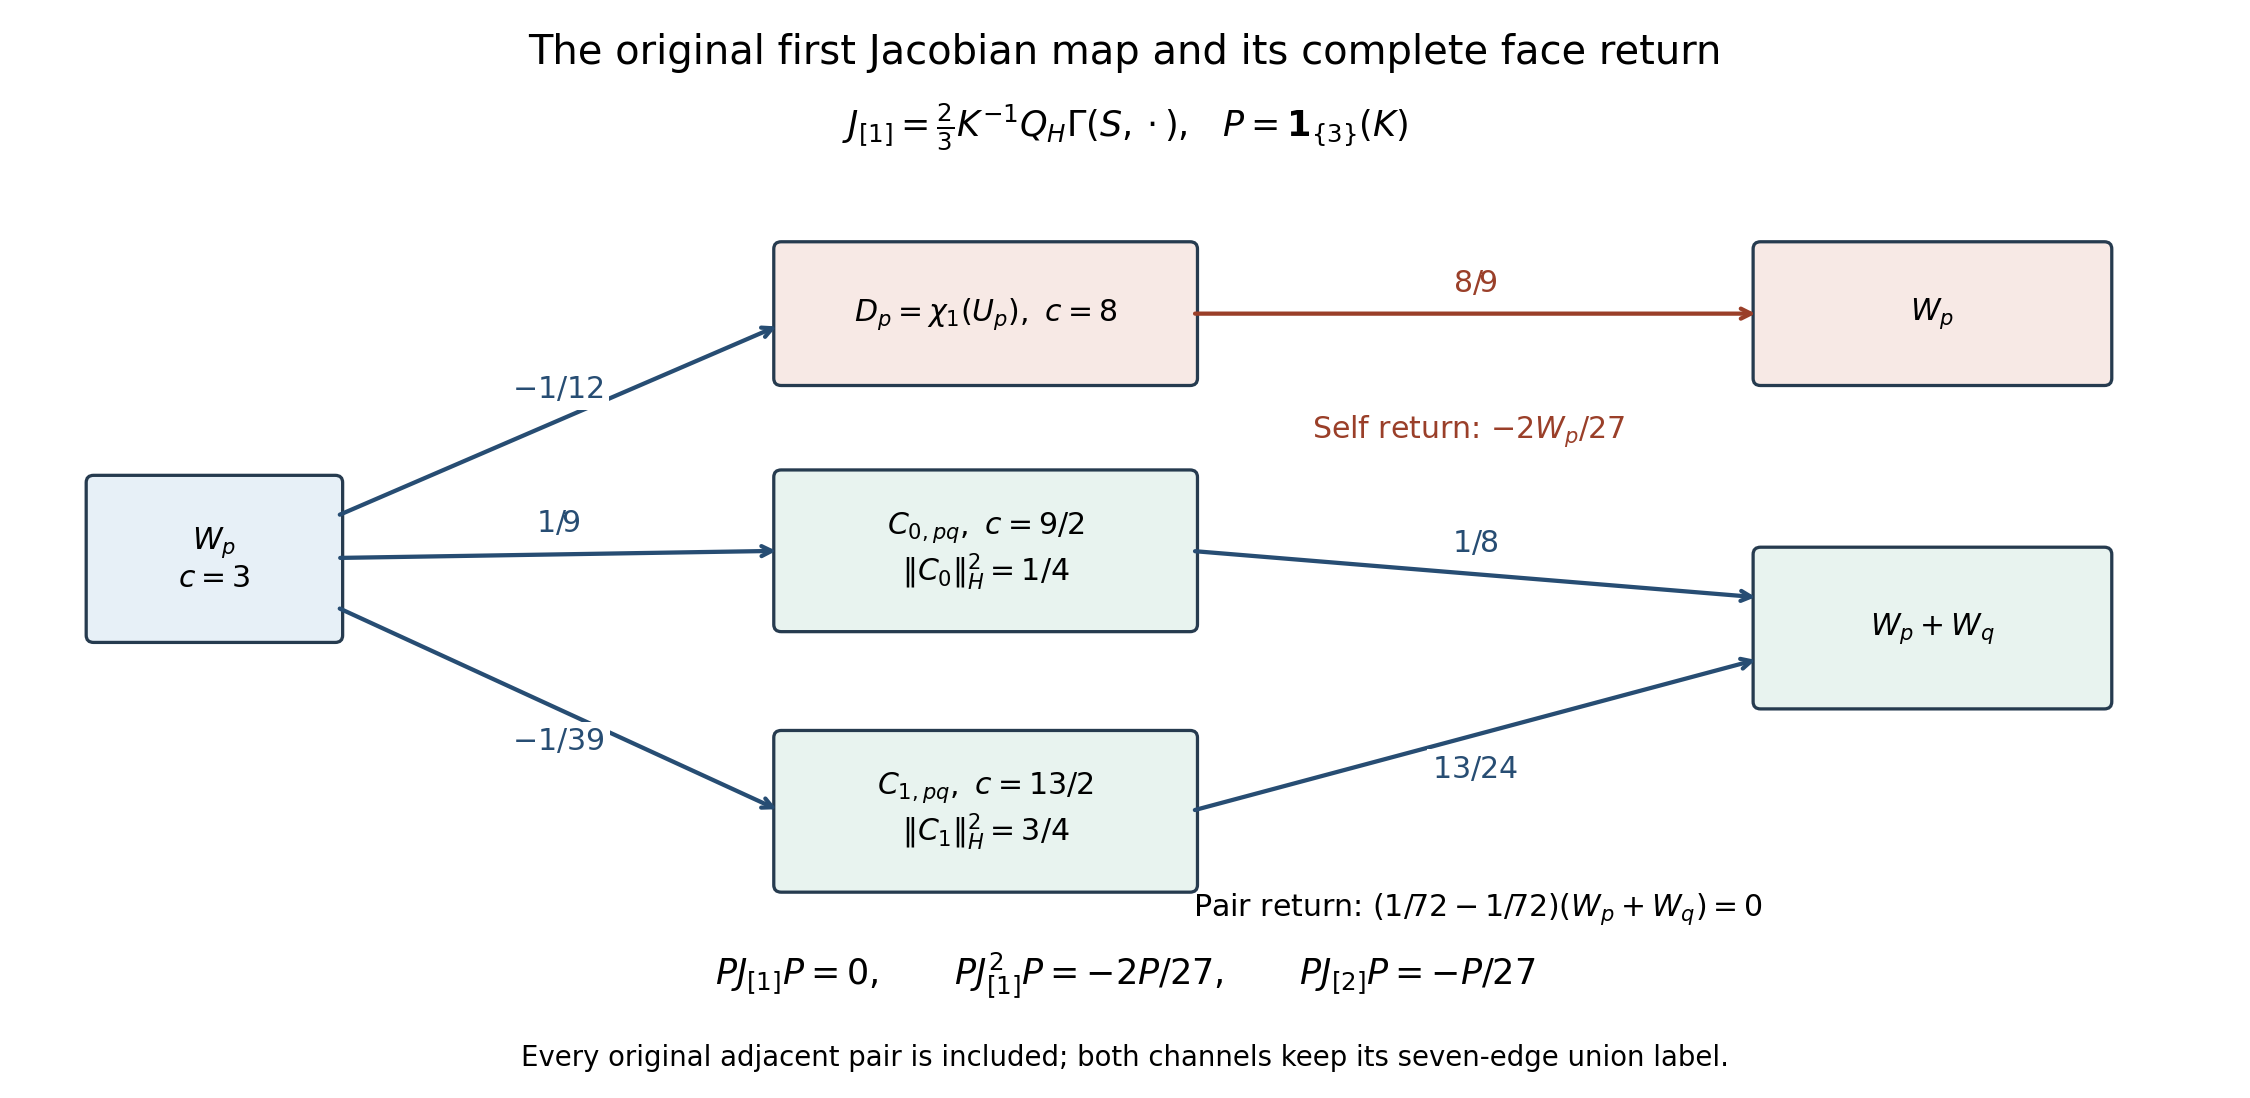
\includegraphics[width=\linewidth,height=.72\textheight,keepaspectratio]{JACOBIAN_RETURN.png}\caption{Original outgoing and return maps}\end{figure}

Figure: the self-face term and one arbitrary adjacent unordered pair in (J1)–(J4). Every actual neighbor is included in the sum (J1); the drawing shows the two common channels of a single pair. Arrows retain the original Casimirs, Haar norms, outgoing signs and return factors. The pair cancels within its original seven-edge union, while the self-face term returns \(-2W_p/27\). The second direct coefficient is separately proved in (J5). Figure source: jacobian\_return\_figure.py, with SVG and inspected PNG beside this note.

The exact outgoing norms and rational return coefficients are independently checked in CLAUDE\_EXACT\_LOCAL\_CHECKS.json. This note supplies the complete arguments for (J1)–(J7); the preserved source supplies the original face-channel and physical free-band proofs. No Lean, new worker, publication, or change of reasoning effort occurred.
\clearpage
\section*{Complete fixed-box spectral weights of the original phase family}

The phase Gram and energy limits IP17 determine two moments. Here the same original vectors give every limiting spectral weight. This also computes the exact part of the oscillator action leaving the degree-three phase space. The calculation retains the fixed-box order of limits; it does not exchange it with the prescribed growing-box path.

The complete providers are \href{https://github.com/KokunoYumeto/yang-mills-interacting-workbench/blob/485b61423c1f4e1805deb453c1b6b342b27842b6/yang-mills/continuations/20260930-s6-ns-moment-map-bridge/PERIOD_COUPLING_AND_PHYSICAL_KERNELS.md#L2434}{PK102–PK112}, including the full Haar/dilation map, and \href{https://github.com/KokunoYumeto/yang-mills-interacting-workbench/blob/256d0fb1988e810df3fcb796c54077c564d48672/yang-mills/continuations/20261011-central-signs-shrinking-window/PHASE_MOMENTS_AND_ORIGINAL_PATH.md}{IP10–IP20}, including actual polynomial-vector convergence and its moment proof. These are retained programme derivations. No novelty claim is made for the Gaussian or Hermite methods used below; their needed identities are proved here.

\subsection*{1. Original operator, coordinates and receiving vectors}

Fix the original open box \(L\ge2\) and \(a>0\), and let \(g\downarrow0\). Retain
\[
 H_g={2g^2\over a}H_0+{1\over2g^2a}\sum_p(2-W_p),\qquad
 A_g=H_g-E_{0,g},\qquad \|\psi_g\|=1,\quad\psi_g>0.
 \tag{SP1}
\]
The exact isometry is
\[
 (\mathcal B_g f)(x)=\mathbf1_{\Omega_g}(x)g^{3d_L/2}
 (16\pi^2)^{-d_L/2}\prod_c{\sin(g|x_c|/2)\over g|x_c|/2}
 f(\exp(gx)),\quad \Omega_g=\{x:|x_c|<2\pi/g\ \forall c\}.
 \tag{SP2}
\]
The sinc factors are positive on this chart and have value one at zero. The map extends by zero. In each colour the original linear map is \(z=O^TG^{-1/2}x\), with absolute Jacobian \((\det G)^{3/2}\) for all colours. The limiting oscillator and its full vacuum are
\[
\begin{split}
 H_{\rm osc}&=\sum_{\nu=1}^{d_L}
 \left[-{2\over a}\Delta_{z_\nu}+{\sigma_\nu^2\over8a}|z_\nu|^2\right],
 &\mu_0&={3\over2a}\sum_{\nu=1}^{d_L}\sigma_\nu,\\
 \Phi_0(x)&=(\det G)^{-3/4}
 \prod_{\nu=1}^{d_L}\left({\sigma_\nu\over4\pi}\right)^{3/4}
 \exp\left[-{1\over8}\sum_{\nu=1}^{d_L}\sigma_\nu|z_\nu|^2\right].
\end{split}\tag{SP3}
\]
All other modes remain in their vacuum. The two selected modes have
\(\sigma_1=\sigma_3=\sigma_* =\sqrt8\sin(\pi/[2(2L+1)])\).
Put
\[
 q={\sigma_*\over2}z_1\cdot z_3,\qquad
 \delta_*={2\sigma_*\over a},\qquad
 X=\sqrt{\sigma_*/2}\,z_1,\quad Y=\sqrt{\sigma_*/2}\,z_3,
 \quad u=|X|^2+|Y|^2.
 \tag{SP4}
\]
The last variables are only integration coordinates. The squared vacuum, with the full Jacobians in SP2–SP3, makes \(X,Y\) independent standard three-dimensional Gaussian vectors. Indeed the factor \((\det G)^{-3/2}\) cancels exactly against \(dx=(\det G)^{3/2}dz\), and each selected density \((\sigma_*/4\pi)^{3/2}e^{-\sigma_*|z|^2/4}dz\) becomes \((2\pi)^{-3/2}e^{-|X|^2/2}dX\). No raw state is replaced or divided by its norm.

For the original index \(b=(p,q_b)\), \(0\le q_b<p\le R\), write
\[
 n_b=p+q_b,\qquad d_b=(-1)^{q_b}-(-1)^p,\qquad
 F_{b,g}=P_{p q_b}(p_g,r_g)\psi_g,
 \quad P_{p q_b}(x,y)=x^py^{q_b}-x^{q_b}y^p.
 \tag{SP5}
\]
Here \(p_g,r_g\) are precisely the original phases, with \(r_g=p_g\circ\mathcal R\). IP15 proves \(\mathcal B_gF_{b,g}\to d_bq^{n_b}\Phi_0\) strongly, including the tails of these unbounded multipliers. The coefficient \(d_b\) is zero for even \(n_b\); these finite-regulator vectors are retained even when their limiting vector is zero.

\subsection*{2. Exact finite spectral expansion}

Conjugating the original oscillator by its positive vacuum gives, on polynomials in the six displayed Gaussian coordinates,
\[
 \Phi_0^{-1}(H_{\rm osc}-\mu_0)\Phi_0
 ={\delta_*\over2}\mathcal N,\qquad
 \mathcal N=-\Delta_X-\Delta_Y+X\cdot\nabla_X+Y\cdot\nabla_Y.
 \tag{SP6}
\]
To check every factor, a selected \(z\)-gradient becomes \(\sqrt{\sigma_*/2}\) times an \(X\)-gradient. The kinetic coefficient therefore becomes \(\sigma_*/a=\delta_*/2\). Expanding the vacuum derivative gives the same coefficient on \(X\cdot\nabla_X\). The constant is exactly the subtracted contribution to \(\mu_0\).

Define the real polynomials \(\operatorname{He}_j\) by
\(e^{tx-t^2/2}=\sum_{j\ge0}\operatorname{He}_j(x)t^j/j!\).
Differentiating this identity gives
\(( -d^2/dx^2+x\,d/dx)\operatorname{He}_j=j\operatorname{He}_j\).
For standard Gaussian \(Z\), integration of the product of two generating functions gives \(\mathbb E[e^{tZ-t^2/2}e^{sZ-s^2/2}]=e^{ts}\); hence
\(\mathbb E[\operatorname{He}_j(Z)\operatorname{He}_k(Z)]=j!\mathbf1_{j=k}\).
Differentiation and integration are justified on a neighbourhood of the origin by the Gaussian density and then identify polynomial coefficients. Multiplying the generating function by \(e^{t^2/2}\) also proves the full finite identity
\[
 x^n=\sum_{h=0}^{\lfloor n/2\rfloor}
 {n!\over2^h h!(n-2h)!}\operatorname{He}_{n-2h}(x).
 \tag{SP7}
\]
Thus each \(q^n\Phi_0\) is a finite sum of orthogonal exact oscillator eigenvectors, with no assumption about a truncated invariant phase space.

For multi-indices \(h,k\in\mathbb N_0^3\), put
\[
 c_n(h,k)=
 \sum_{\substack{\alpha\in\mathbb N_0^3,\ |\alpha|=n\\
                 \alpha_i\ge h_i,k_i;\ \alpha_i-h_i,\alpha_i-k_i\in2\mathbb N_0}}
 {n!\over\alpha!}
 \prod_{i=1}^3
 {\alpha_i!\over2^{(\alpha_i-h_i)/2}((\alpha_i-h_i)/2)!h_i!}
 {\alpha_i!\over2^{(\alpha_i-k_i)/2}((\alpha_i-k_i)/2)!k_i!}.
 \tag{SP8}
\]
The sum over an empty set is zero. Expanding \((\sum_iX_iY_i)^n\) by the multinomial formula and applying SP7 to each of its six factors proves that \(c_n(h,k)\) is its complete Hermite coefficient. In particular \(|h|\) and \(|k|\) have the parity of \(n\). For odd \(n\), both are at least one. Define
\[
 W_\ell(n,m)=
 \sum_{\substack{h,k\in\mathbb N_0^3\\ |h|+|k|=2\ell}}
 c_n(h,k)c_m(h,k)h!k! .
 \tag{SP9}
\]
Each sum is finite; it vanishes for \(\ell>\min(n,m)\), and for \(\ell=0\) when either index is odd. SP6–SP8 prove that this is exactly the cross Gram entry of the two vectors' projections onto excitation \(\ell\delta_*\). Consequently the original phase-family spectral matrices are
\[
 (\mathsf W_\ell)_{bc}=d_bd_c W_\ell(n_b,n_c),\qquad
 \mathcal G^{(0)}=\sum_\ell\mathsf W_\ell,\quad
 \mathcal C^{(0)}=\delta_*\sum_\ell\ell\mathsf W_\ell,\quad
 \mathcal D^{(0)}=\delta_*^2\sum_\ell\ell^2\mathsf W_\ell.
 \tag{SP10}
\]
The simultaneous colour rotations commute with the full oscillator, so each spectral component of the invariant original vector is still physical; no individual noninvariant Hermite tensor is being declared physical. Every \(\mathsf W_\ell\) is positive semidefinite, since SP9 is a weighted Gram formula, including the original signs \(d_b\). The last matrix is the full oscillator second moment. No convergence of the unbounded actual second moments is being inferred merely from norm convergence.

For a useful closed generating expression set \(z=e^{-t\delta_*}\), \(t\ge0\). Then
\[
 \sum_{n,m\ge0}{v^nw^m\over n!m!}
       \sum_{\ell\ge0}W_\ell(n,m)z^\ell
 =\left[1-v^2-w^2-2zvw+(1-z)^2v^2w^2\right]^{-3/2}.
 \tag{SP11}
\]
Here the equality holds analytically for \(v,w\) sufficiently small, and equivalently as a formal power series. Its proof retains every determinant term. Couple \(X' =\rho X+\sqrt{1-\rho^2}\,\widehat X\) and \(Y'=\rho Y+\sqrt{1-\rho^2}\,\widehat Y\), with four independent standard triples and \(\rho=e^{-t\delta_*/2}\). Conditional integration of the Hermite generating function gives \(\mathbb E[\operatorname{He}_h(X')\mid X]=\rho^h\operatorname{He}_h(X)\) in each coordinate. Thus the left side is \(\mathbb E e^{vX\cdot Y+wX'\cdot Y'}\).
For one colour rotate to \(A=(X+Y)/\sqrt2\), \(B=(X-Y)/\sqrt2\) and their primed partners. The two resulting pairs are independent and each has covariance \(C=\left(\begin{smallmatrix}1&\rho\\\rho&1\end{smallmatrix}\right)\). Gaussian integration of the positive and negative quadratic forms gives the two determinants
\(\det(I-C\operatorname{diag}(v,w))=1-v-w+(1-\rho^2)vw\) and
\(\det(I+C\operatorname{diag}(v,w))=1+v+w+(1-\rho^2)vw\).
This follows directly by completing the quadratic form in its Gaussian integral; its determinant factor has power \(-1/2\). Multiply both determinants, then take the product over the three independent colours. This gives SP11 with \(z=\rho^2\). At \(\rho=1\) the same formula follows by a limit of the integrable Gaussian exponential, or direct integration with \(X'=X,Y'=Y\).

\subsection*{3. Every actual fixed-box cluster weight}

For each of the finitely many \(\ell\) with \(\mathsf W_\ell\ne0\), choose an interval \(I_\ell\) around \(\ell\delta_*\) containing no other oscillator excitation value and with endpoints outside its spectrum. The complete oscillator is discrete at fixed box, so these intervals exist even if other modes share the same central eigenvalue. The retained norm convergence of finite spectral projections and SP5 imply
\[
 \langle F_{b,g},\mathbf1_{I_\ell}(A_g)F_{c,g}\rangle
       \longrightarrow(\mathsf W_\ell)_{bc},\qquad
 \left\|\left(I-\sum_\ell\mathbf1_{I_\ell}(A_g)\right)F_{b,g}\right\|^2
       \longrightarrow0.
 \tag{SP12}
\]
For the first assertion apply the transported projection to each convergent vector; add and subtract its limiting projection and use norm at most one. For the second, the intervals are disjoint, so the squared complement norm is the full norm minus the finite sum of its projected squared norms. SP5 and SP10 make its limit zero. No individual equality or degeneracy of the higher interacting eigenvalues is asserted: each interval includes its entire actual cluster.

These identities also prove weak convergence of the actual finite spectral measures for all bounded continuous test functions. To see this directly, given a finite linear combination of the original vectors, shrink each interval so the test function differs from its central value by at most a prescribed tolerance. The omitted complement mass tends to zero by SP12; the contribution in the intervals is bounded by that tolerance times the bounded total raw norm. Polarization proves the cross-measure statement. In particular all original phase-family Laplace matrices converge to \(\sum_\ell e^{-t\ell\delta_*}\mathsf W_\ell\) for each \(t\ge0\). This conclusion retains fixed \(L,a\); no volume-independent rate follows.

\subsection*{4. The exact degree-three return to the missing radial variable}

In original order \((1,0),(2,0),(2,1)\), the limiting vectors are \(2q\Phi_0,0,-2q^3\Phi_0\). Their complete spectral matrices are
\[
 \mathsf W_1=\begin{pmatrix}12&0&-180\\0&0&0\\-180&0&2700\end{pmatrix},\quad
 \mathsf W_2=\begin{pmatrix}0&0&0\\0&0&0\\0&0&2160\end{pmatrix},\quad
 \mathsf W_3=\begin{pmatrix}0&0&0\\0&0&0\\0&0&1440\end{pmatrix}.
 \tag{SP13}
\]
All other matrices are zero. Here is an independent full polynomial derivation. The original differential operator gives
\[
 \mathcal N q=2q,\quad
 \mathcal N(uq)=4uq-20q,\quad
 \mathcal N(q^3)=6q^3-6uq.
 \tag{SP14}
\]
For example \(\Delta u=12\), \(\nabla u\cdot\nabla q=4q\), \(|\nabla q|^2=u\) and \(\Delta q=0\), so every contraction and coefficient in SP14 is explicit. The three nonzero orthogonal eigenpolynomials are
\[
 e_1=q,\qquad e_2=uq-10q,\qquad
 e_3=q^3-3uq+15q,\qquad q^3=15e_1+3e_2+e_3,
 \tag{SP15}
\]
with excitation energies \(\delta_*,2\delta_*,3\delta_*\), respectively. Their squared Gaussian norms are \(3,60,360\). To verify these without omitting moments, conditional Gaussian integration gives \(\mathbb E q^2=3\), \(\mathbb E q^4=45\), \(\mathbb E q^6=1575\). Gaussian integration by parts gives \(\mathbb E(uq^2)=30\). In six-dimensional polar coordinates the radius square \(u\) has density proportional to \(u^2e^{-u/2}\), while \(q^2\) is homogeneous of degree four; the ratio of its two radial integrals gives \(\mathbb E(u^2q^2)=120\mathbb E q^2=360\). Thus \(\|e_2\|^2=360-20\cdot30+100\cdot3=60\). Orthogonality follows from the self-adjoint oscillator and its distinct energies; all vectors are polynomials times its Gaussian and in its domain. Finally \(\|e_3\|^2=1575-15^2\cdot3-3^2\cdot60=360\). SP13 follows by retaining the factors \(2,-2\).

The full second oscillator moment and the exact energy-compression defect are therefore
\[
 \mathcal D^{(0)}=\delta_*^2
 \begin{pmatrix}12&0&-180\\0&0&0\\-180&0&24300\end{pmatrix},\qquad
 \mathcal D^{(0)}-\mathcal C^{(0)}(\mathcal G^{(0)})^+
                      \mathcal C^{(0)}
 =\delta_*^2\begin{pmatrix}0&0&0\\0&0&0\\0&0&864\end{pmatrix}.
 \tag{SP16}
\]
The superscript \(+\) is the Moore–Penrose inverse on this explicitly known limiting Gram matrix, including its zero row. It does not replace any finite-regulator inverse or assert convergence of those inverses. To prove the defect geometrically, let \(V\) map the three original coefficient coordinates to the three displayed oscillator vectors, and let \(\Pi\) be the orthogonal projection onto their span. Then \(\mathcal G^{(0)}=V^*V\), \(\mathcal C^{(0)}=V^*A_{\rm osc}V\), \(\Pi=V(\mathcal G^{(0)})^+V^*\), and the difference is exactly \(V^*A_{\rm osc}(I-\Pi)A_{\rm osc}V\). Thus SP16 is the squared norm of an actual connecting operator, not merely the nonidentity of two spaces.

The original combination \(F_{21}+15F_{10}\) has limiting squared norm \(3600\), energy moment \(8640\delta_*\), and spectral masses \(2160,1440\) at \(2\delta_*,3\delta_*\). Its energy quotient is \((12/5)\delta_*\); its spectral variance divided by the same raw norm is \((6/25)\delta_*^2\). The omitted radial direction is therefore essential. In fact SP14–SP15 prove that the smallest oscillator-invariant linear space containing \(q^3\Phi_0\) is exactly \(\operatorname{span}\{q\Phi_0,uq\Phi_0,q^3\Phi_0\}\): three distinct nonzero projections require dimension at least three, and the displayed span is invariant. These are exact maps and norms of the original limiting vectors.

The resulting next calculation on the joint path still requires estimates uniform in the growing box for the actual interacting vacuum and cluster maps. SP9–SP16 supply the complete fixed-box target matrices, including their complementary return. They do not provide that uniform estimate or identify the continuum theory.


\begin{figure}[htbp]\centering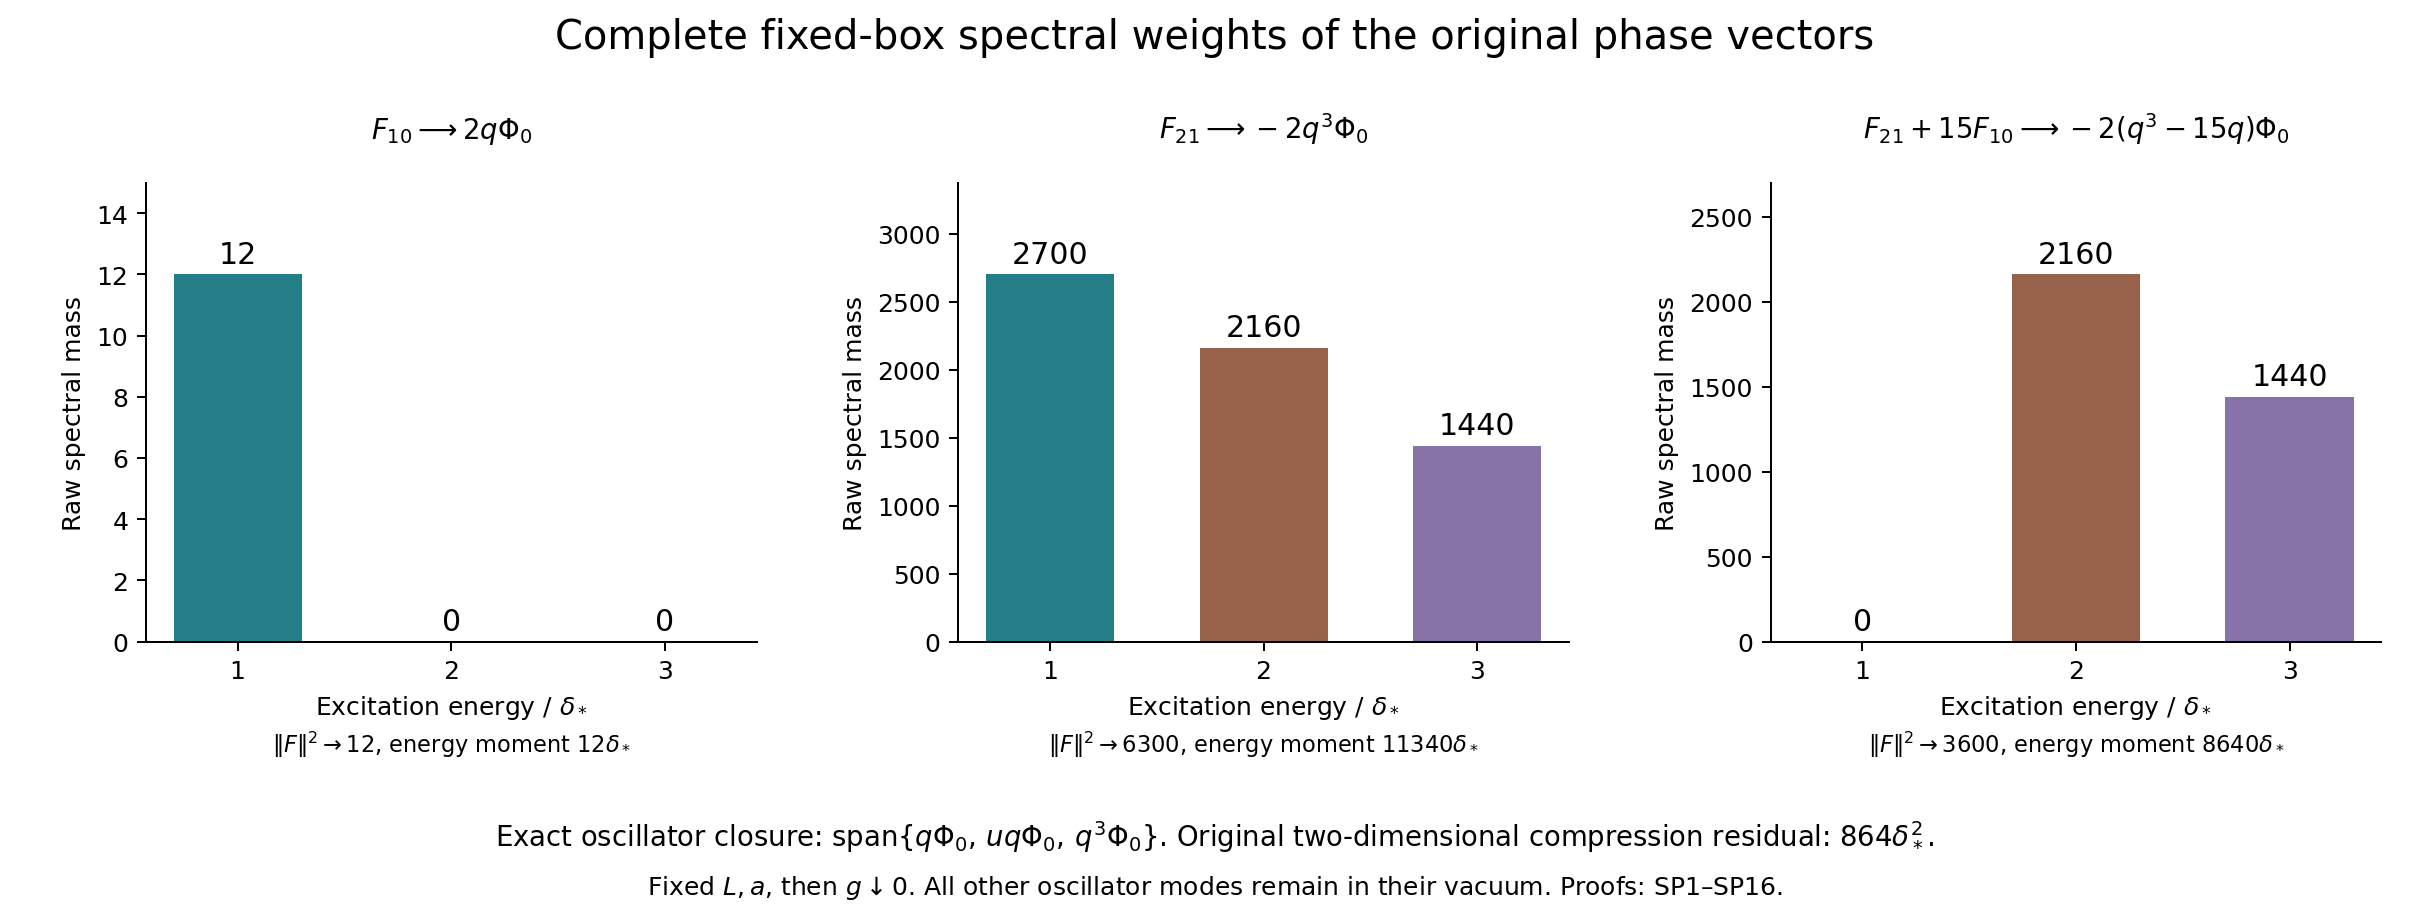
\includegraphics[width=\linewidth,height=.72\textheight,keepaspectratio]{PHASE_SPECTRAL_WEIGHTS.png}\caption{Complete raw spectral weights and the missing radial direction}\end{figure}

The three panels show the exact raw masses in SP13–SP16, with separate vertical scales. The third panel retains the original coefficient 15. Its two occupied energies produce the quotient 12δ*/5. The full original oscillator and its vacuum remain SP3. Reproducible source: phase\_spectrum\_figure.py.
\clearpage
\section*{Exact boundary reflection and the original raw endpoint}

This continues IP1–IP22 while retaining the actual vacuum, original
polynomial \(F=p-r\), and prescribed simultaneous path. The calculation
locates the full nonlinear reflection correction, computes its entire
normal kinetic form at identity boundary holonomies, and obtains an
actual-vacuum lower bound for the energy of that correction. It does not
settle the sign of the original shrinking-window endpoint.
The strongest evaluated bounds are (JP43) for the even correction
energy and (JP47) for the original odd raw mass and energy. Their
original-path exponential loss is proportional to \(j^2\).

\subsection*{1. Original links and the two tree presentations}

Retain the original box, root, tree, coefficients and coordinates of
\href{https://github.com/KokunoYumeto/yang-mills-interacting-workbench/blob/485b61423c1f4e1805deb453c1b6b342b27842b6/yang-mills/continuations/20260930-s6-ns-moment-map-bridge/PERIOD_COUPLING_AND_PHYSICAL_KERNELS.md#L2440}{PK103–PK108}
and \href{https://github.com/KokunoYumeto/yang-mills-interacting-workbench/blob/485b61423c1f4e1805deb453c1b6b342b27842b6/yang-mills/continuations/20260930-s6-ns-moment-map-bridge/PERIOD_COUPLING_AND_PHYSICAL_KERNELS.md#L3500}{PK158–PK160}.
Thus \(m=2L\), \(n=m+1\), \(L\ge2\); a vertex `(i,k,l)` represents
the physical point \(o+a(i-L,k-L,l-L)\). The tree contains every
direction-one edge, direction-two edges with \(i=0\), and direction-three
edges with \(i=k=0\). Its root path goes first in direction three, then
two, then one. Every original rooted word is still
\(Z_c=t_sU_ct_t^{-1}\).

Use the exact tree-gauge coordinate map: original tree links equal
identity and chord links equal their original based words \(Z_c\).
This is a coordinate presentation of the gauge-invariant functions,
not a replacement configuration or vacuum. Put
\[
\begin{array}{ll}
 U_2(i,k,l)=Z_{(i,k,l;2)}&(i\ge1),\qquad U_2(0,k,l)=I,\\
 U_3(i,k,l)=Z_{(i,k,l;3)}&((i,k)\ne(0,0)),\quad U_3(0,0,l)=I.
\end{array}\tag{JP1}
\]
The chord families have their original endpoint restrictions:
\(0\le k<m,0\le l\le m\) for direction two and
\(0\le i,k\le m,0\le l<m\) for direction three.

The complete original coefficient rows are as follows:
\[
\begin{gathered}
 h={\pi\over2n},\qquad v_0(l)=n^{-1/2},\qquad
 v_1(l)=\sqrt{2/n}\cos{\pi(l+1/2)\over n},\qquad
 w_1(l)=-\sqrt{2/n}\sin{\pi(l+1)\over n},\\
 a_{(i,k,l;2)}=\mathsf M_{1,(i,k,l;2)}
             =-{v_1(i)w_1(k)v_0(l)\over\sqrt2},\qquad
 a_{(i,k,l;3)}=\mathsf M_{1,(i,k,l;3)}=0,\\
 b_{(i,k,l;2)}=\mathsf M_{3,(i,k,l;2)}
             ={v_0(i)w_1(k)v_1(l)\over\sqrt2},\qquad
 b_{(i,k,l;3)}=\mathsf M_{3,(i,k,l;3)}
             =-{v_0(i)v_1(k)w_1(l)\over\sqrt2},\\
 S_1=\sum_c|a_c|
       =\sqrt{2/n}\cot h(\cot h-\cos h),\\
 S_3=\sum_c|b_c|
       =\sqrt{2/n}\big[(2-1/n)\cot^2h-(\cos h/n)\cot h\big].
\end{gathered}
\]
Here \(v_0,v_1\) have vertex indices \(0,\ldots,m\), and \(w_1\)
has edge indices \(0,\ldots,m-1\). Every row is restricted to the
original chords in (JP1). The absolute sums are evaluated with all
excluded tree edges retained as exclusions; their finite trigonometric
summations are proved in
\href{https://github.com/KokunoYumeto/yang-mills-interacting-workbench/blob/256d0fb1988e810df3fcb796c54077c564d48672/yang-mills/continuations/20261011-central-signs-shrinking-window/PHASE_MOMENTS_AND_ORIGINAL_PATH.md#L108}{IP2–IP4}.

Retain \(N=3m(m+1)^2\), \(M=3m^2(m+1)\) and the complete physical
Hamiltonian
\[
 H=\kappa H_0+b_{\rm mag}W,\quad
 H_0=-\sum_{e,\alpha}X_{e,\alpha}^2,\quad
 W=\sum_{\text{all faces }p}(2-\operatorname{tr}U_p),\quad
 \kappa={2g^2\over a},\quad b_{\rm mag}={1\over2g^2a},
 \quad \xi={b_{\rm mag}\over\kappa}={1\over4g^4}.
\]
The positive unit vacuum is \(H\psi=E_0\psi\), \(d\mu=\psi^2dU\);
the term \(2b_{\rm mag}M\) remains in this potential. Define
\[
 \sigma_*=\sqrt8\sin h,\quad\beta_0={\sigma_*\over2g^2},\qquad
 p=\beta_0\mathcal S,\quad r=\beta_0\mathcal S_{\mathcal R},
 \quad F=p-r,\qquad
 \mathcal Q_4=\mu(\mathcal S^2),\
 \mathcal Q_{4,\mathcal R}=\mu(\mathcal S\mathcal S_{\mathcal R}),\
 \mathcal K_1=\mu(|\nabla\mathcal S|^2),\
 \mathcal K_{\mathcal R}
   =\mu(\nabla\mathcal S\cdot\nabla\mathcal S_{\mathcal R}),
\]
where the vectors defining \(\mathcal S\) occur below. The exact
ground-state form is
\(\langle F\psi,(H-E_0)F\psi\rangle
=\kappa\mu(|\nabla F|^2)\).
Its proof multiplies the complete vacuum equation by \(F^2\psi\),
integrates by parts on the compact link product, and subtracts it
from the product-rule expression for
\(\langle F\psi,H F\psi\rangle-E_0\mu(F^2)\).
The two mixed derivatives and the \(F^2|\nabla\psi|^2\) terms then
cancel exactly, as do the full potential and energy terms.
Reflection invariance makes \(F\psi\) odd and vacuum orthogonal.
The original raw shrinking-window expression is
\[
 \mathscr E(s)=\mu(F^2)-{\kappa\over s}\mu(|\nabla F|^2)
 =2\beta_0^2(\mathcal Q_4-\mathcal Q_{4,\mathcal R})
   -{2\kappa\beta_0^2\over s}(\mathcal K_1-\mathcal K_{\mathcal R}).
\]
The spectral theorem gives
\(\langle F\psi,\mathbf1_{(0,s]}(H-E_0)F\psi\rangle
\ge\max\{0,\mathscr E(s)\}\). The requested joint path is
\(L_j=j^4,\ a_j=1/(100j),\
g_j^2=\kappa_*/(200j),\ s_j=\kappa_*/j\), so
\(\kappa_j=\kappa_*>0\). All subsequent path statements concern
this same \(F_j\psi_j\) and these exact coefficients, for \(j\ge2\).

Define the exact boundary set
\[
\mathcal B_2=\{(m,k,l;2):0\le k<m,0\le l\le m\},\qquad
\mathcal B_3=\{(m,0,l;3):0\le l<m\},\qquad
\mathcal B=\mathcal B_2\sqcup\mathcal B_3.
\tag{JP2}
\]
It has \(m(m+1)+m=m(m+2)=n^2-1\) members. These are exactly the
original chords that become tree links under the direction-one
reflection. No boundary face or direction-three member is omitted.

For every `(k,l)` define the ordered matrix products
\[
 B_l=\prod_{r=0}^{l-1}U_3(m,0,r),\qquad
 A_{k,l}=B_l\prod_{b=0}^{k-1}U_2(m,b,l),
\tag{JP3}
\]
where factors occur in increasing index order and empty products equal
identity. In the original tree-gauge coordinates the exact reflected
rooted words are
\[
\boxed{
\begin{split}
 Z^{\mathcal R}_{(i,k,l;2)}
    &=A_{k,l}U_2(m-i,k,l)A_{k+1,l}^{-1},\\
 Z^{\mathcal R}_{(i,k,l;3)}
    &=A_{k,l}U_3(m-i,k,l)A_{k,l+1}^{-1}.
\end{split}}\tag{JP4}
\]
To prove this, reflect each edge of the original root path. Its
direction-three segment lies at \(i=m,k=0\), its direction-two segment
at \(i=m\), and its reversed direction-one segment consists of original
tree links, hence identity in this exact coordinate presentation. The
first two segments are exactly (JP3). The reflected chord is the
corresponding link with first index \(m-i\), in the same orientation
because its direction is two or three. The final root segment is the
inverse of the complete endpoint product, proving both lines. In
particular the direction-three endpoint is \(A_{k,l+1}\), not a
commuted or abbreviated product of the direction-two factors at level
\(l\).

The reflected target link in (JP4) never belongs to \(\mathcal B\).
For direction two that would require \(i=0\), excluded from its chord
set. For direction three it would require \((i,k)=(0,0)\), likewise
excluded. A reflected target may be an original tree link, in which
case (JP1) retains its identity value. Thus all boundary dependence in
(JP4) occurs through its two endpoint transport products. This proves
the exact relation between the original tree coordinates and the
reflected ones on the whole compact configuration space.

\subsection*{2. Exact colour-vector transport and the reflection correction}

For \(U\in SU(2)\), write
\(U=c(U)I+\sum_\alpha q^\alpha(U)T_\alpha\), with
\(c(U)=\operatorname{tr}U/2\) and \(T_\alpha=-i\sigma_\alpha/2\).
The original coordinate is \(q^\alpha=-2\operatorname{tr}(T_\alpha U)\).
Quaternion multiplication, with all signs retained, is
\[
 q(UV)=c(V)q(U)+c(U)q(V)+\tfrac12q(U)\times q(V).
 \tag{JP5}
\]
Indeed \(T_\alpha T_\beta=-\delta_{\alpha\beta}I/4
+\epsilon_{\alpha\beta\gamma}T_\gamma/2\); multiplying the full
matrices gives precisely this vector coefficient and the scalar
coefficient \(c(U)c(V)-q(U)\cdot q(V)/4\).

For a reflected chord with endpoints \(s=(k,l)\), \(t=(k+1,l)\)
or \((k,l+1)\), define
\[
 V_c=A_sA_t^{-1},\quad v_c=q(V_c),\quad c_c=c(V_c),\quad
 R_c=\operatorname{Ad}_{A_s}\in SO(3),\quad
 U_{\bar c}=U_2(m-i,k,l)\text{ or }U_3(m-i,k,l).
\]
Then (JP4)–(JP5) give the full affine quaternion formula
\[
\boxed{
 q_c^{\mathcal R}
 =c_cR_cq(U_{\bar c})+c(U_{\bar c})v_c
       +\tfrac12[R_cq(U_{\bar c})]\times v_c.}
\tag{JP6}
\]
It includes the scalar component of each original chord. Dropping that
component, either cross product, or an endpoint transport changes the
reflection map.

Use the original coefficients \(a_c=\mathsf M_{1c}\),
\(b_c=\mathsf M_{3c}\), and write
\(u_1^{\mathcal R}=\sum_ca_cq_c^{\mathcal R}\),
\(u_3^{\mathcal R}=\sum_cb_cq_c^{\mathcal R}\).
For clarity, define the errors as exact functions, not assumed small:
\[
\begin{split}
 e_1&=u_1^{\mathcal R}+u_1
   =\sum_ca_c[q_c^{\mathcal R}-q(U_{\bar c})]
       +\sum_{b\in\mathcal B_2}a_bq_b,\\
 e_3&=u_3^{\mathcal R}-u_3
   =\sum_cb_c[q_c^{\mathcal R}-q(U_{\bar c})]
       -\sum_{b\in\mathcal B}b_bq_b.
\end{split}\tag{JP7}
\]
To check every boundary sign, change the index \(i\) to \(m-i\).
The direction-two first-row coefficient changes sign because
\(v_1(m-i)=-v_1(i)\). Its reflected sum misses the original \(i=m\)
row and includes the original identity tree row \(i=0\), giving
\(-u_1+\sum_{\mathcal B_2}a_bq_b\). The third-row coefficient is
independent of \(i\), so its direction-two sum misses exactly
\(\mathcal B_2\). Its direction-three sum misses exactly
\(\mathcal B_3\) and includes the original identity tree links.
Adding the affine errors yields (JP7).

Set \(\mathcal S=u_1\cdot u_3\),
\(\mathcal S_{\mathcal R}=u_1^{\mathcal R}\cdot u_3^{\mathcal R}\),
and retain the complete reflection correction
\[
 D:=\mathcal S+\mathcal S_{\mathcal R}
   =e_1\cdot u_3-u_1\cdot e_3+e_1\cdot e_3.
 \tag{JP8}
\]
The last equality is the full product expansion of
\((-u_1+e_1)\cdot(u_3+e_3)\). All three terms remain.
On the exact fibre
\[
 \mathcal Z_{\mathcal B}
   =\{Z_b=I\text{ for every }b\in\mathcal B\}
\]
every \(A_s,V_c\) is identity, so \(e_1=e_3=0\) and \(D=0\).
Every other original chord on this fibre is arbitrary. Thus the failure
of the global reflection sign has an exact boundary-variable description;
it is not a statement that the reflected and original phase are unrelated.

\subsection*{3. The full normal derivative on that fibre}

The vanishing of \(D\) on \(\mathcal Z_{\mathcal B}\) does not imply
vanishing physical gradient there. We now compute every normal derivative
and its complete physical kinetic metric.

For a boundary chord \(b\), let \(\epsilon_{s,b}\) equal one if its
matrix occurs in the ordered product \(A_s\) of (JP3), and zero otherwise.
Every such product traverses a boundary edge at most once and in positive
orientation. Put
\(\chi^-_{cb}=\epsilon_{s,b}-\epsilon_{t,b}\),
\(\chi^+_{cb}=\epsilon_{s,b}+\epsilon_{t,b}\).
At \(\mathcal Z_{\mathcal B}\), differentiation of the complete
reflected matrix product in (JP4) gives
\[
 X_{b,\alpha}q_c^{\mathcal R}
   =\chi^-_{cb}c(U_{\bar c})\mathbf e_\alpha
       +\tfrac12\chi^+_{cb}\,\mathbf e_\alpha\times q(U_{\bar c}).
 \tag{JP9}
\]
Here \(X_{b,\alpha}\) is the original left field on the physical chord
link \(b\). The target link is never in \(\mathcal B\), as proved
above. At boundary identity the differentiated left endpoint contributes
\(\epsilon_{s,b}T_\alpha U_{\bar c}\), and the differentiated inverse
right endpoint contributes \(-\epsilon_{t,b}U_{\bar c}T_\alpha\).
The vector coefficients of these products are respectively
\(c(U)\mathbf e_\alpha+\mathbf e_\alpha\times q(U)/2\) and
\(c(U)\mathbf e_\alpha-\mathbf e_\alpha\times q(U)/2\).
Subtract them with their displayed multiplicities to obtain (JP9).

For \(\mu=1,3\), define the original finite sums
\[
 a_{\mu b}^{\partial}
   =\sum_c\mathsf M_{\mu c}\chi^-_{cb}c(U_{\bar c}),\qquad
 v_{\mu b}^{\partial}
   =\tfrac12\sum_c\mathsf M_{\mu c}\chi^+_{cb}q(U_{\bar c}).
\]
Denote by \(n_b\in\mathbb R^3\) the vector with components
\(X_{b,\alpha}D\) on the boundary-identity fibre. Since there
\(u_1^{\mathcal R}=-u_1\), \(u_3^{\mathcal R}=u_3\), the complete
product rule gives
\[
\boxed{
 n_b=(\mathsf M_{1b}+a_{1b}^{\partial})u_3
       +(\mathsf M_{3b}-a_{3b}^{\partial})u_1
       +v_{1b}^{\partial}\times u_3
       -v_{3b}^{\partial}\times u_1.}
\tag{JP10}
\]
The direct derivatives of the original vectors are
\(X_{b,\alpha}u_\mu=\mathsf M_{\mu b}\mathbf e_\alpha\).
For the reflected vectors, insert (JP9); for example
\((\mathbf e_\alpha\times v_{1b}^{\partial})\cdot u_3
=\mathbf e_\alpha\cdot(v_{1b}^{\partial}\times u_3)\).
This proves all four terms and both cross-product signs in (JP10).

Let \(T_{be}\) be the signed sum of all occurrences of physical link
\(e\) in the original full rooted word \(Z_b\), with its inverse
traversals having negative sign. These are exactly the rows of the
original tangent incidence matrix indexed by \(\mathcal B\).
On \(\mathcal Z_{\mathcal B}\), all nonboundary chord derivatives of
\(D\) vanish because its restriction to that entire fibre is zero.
Every original boundary word consists only of original tree links and
its own boundary chord, all identity at this configuration. Therefore
the exact derivative of that word is
\(X_{e,\alpha}Z_b=T_{be}T_\alpha\). It follows that
\[
 X_{e,\alpha}D=\sum_{b\in\mathcal B}T_{be}n_b^\alpha,\qquad
 |\nabla D|^2=\sum_{\alpha=1}^3
   (n^\alpha)^{\mathsf T}G_{\mathcal B}n^\alpha,
 \quad G_{\mathcal B}=T_{\mathcal B}T_{\mathcal B}^{\mathsf T}.
\tag{JP11}
\]
This includes every original physical link, including all tree links.
It is not just the Euclidean chord-gradient norm.

The full matrix in (JP11) can be evaluated exactly. Regard \(\mathcal B\)
as edges of the comb-shaped tree on the \(n^2\) vertices `(k,l)` of the
right wall: it contains every direction-two edge at every height and
the direction-three spine at \(k=0\). Let \(D_{\rm wall}\) be its
oriented edge-to-vertex incidence matrix, with \(-1\) at its starting
vertex and \(+1\) at its ending vertex. Then
\[
\boxed{G_{\mathcal B}=2I+mD_{\rm wall}D_{\rm wall}^{\mathsf T}.}
\tag{JP12}
\]
For proof, expand each original boundary word into signed physical
occurrences before adding them. Common root prefixes occur once forward
and once backward; their signed derivatives cancel exactly. The remaining
cycle consists of its right-wall edge, its oppositely oriented left-wall
tree counterpart, a direction-one path of length \(m\) at the starting
wall vertex, and the reverse direction-one path at the endpoint. Distinct
boundary chords have distinct right- and left-wall edge counterparts,
giving the term \(2I\). Horizontal paths at different wall vertices are
disjoint. Two cycles' shared horizontal contributions therefore have
inner product \(m\) times the corresponding incidence-row inner product.
This proves (JP12) from the entire original words and their signs.

Equivalently the diagonal is \(2m+2\); adjacent direction-two edges
on the same height have entry \(-m\); adjacent spine edges have entry
\(-m\). A direction-two edge `(k,l;2)` and a spine edge `(l';3)` have
entry \(m\mathbf1_{k=0}(\mathbf1_{l=l'}-\mathbf1_{l=l'+1})\).
All other entries vanish. This lists every off-diagonal boundary term.
The tree incidence has full row rank: a putative linear dependence can
be removed successively at a leaf, where its incident coefficient must
be zero. In particular \(G_{\mathcal B}>2I\) as a finite matrix, and
the unconditional inequalities
\[
 2\sum_b|n_b|^2\le |\nabla D|^2
          \le(2+6m)\sum_b|n_b|^2
 \quad\text{on }\mathcal Z_{\mathcal B}
 \tag{JP13}
\]
follow. For the upper bound, every wall-tree vertex has degree at most
three; the sum of squared differences over its edges is at most six
times the vertex squared norm, using \((x-y)^2\le2x^2+2y^2\).
The nonzero singular values of \(D_{\rm wall}\) and its transpose
coincide, proving the required upper matrix bound.

The exact linear receiving map on the normal data space is
\(J_{\mathcal B}=T_{\mathcal B}^{\mathsf T}\otimes I_3\),
from \(\mathbb R^{3|\mathcal B|}\) to the original
\(\mathbb R^{3N}\) of physical link derivatives. Its squared metric
is \(G_{\mathcal B}\otimes I_3\); its inverse on its range is
\((G_{\mathcal B}^{-1}T_{\mathcal B})\otimes I_3\), and the
orthogonal projection onto that range is
\((T_{\mathcal B}^{\mathsf T}G_{\mathcal B}^{-1}T_{\mathcal B})
\otimes I_3\). Multiplication of these matrices proves the inverse
and the self-adjoint idempotent projection, using the positive
invertibility already established. This specifies the complete normal
space and its injection into the physical derivatives.

\subsection*{4. A nonzero normal derivative with every original coefficient}

We evaluate (JP10) at a concrete original configuration. Set every
physical link to identity except the direction-two chord `(1,0,0;2)`,
whose value is \(K_*=\exp(\pi T_1)=2T_1\). All boundary chords are
identity. Vary only the boundary chord `(m,0,0;2)` through
\(H_b(t)=\exp(tT_1)\), keeping the original physical tree identity.
With \(h=\pi/(2n)\), retain the original cochains
\(v_0(l)=n^{-1/2}\),
\(v_1(l)=\sqrt{2/n}\cos(\pi(l+1/2)/n)\), and
\(w_1(l)=-\sqrt{2/n}\sin(\pi(l+1)/n)\).
Define the exact original coefficients and separate scalar functions
\[
 d_0={v_0(0)w_1(0)v_1(0)\over\sqrt2},\qquad
 A=-{v_1(1)w_1(0)v_0(0)\over\sqrt2},\qquad
 \eta(t)=2\sin(t/2),\quad \zeta_*=2,\quad \omega(t)=2\cos(t/2).
\]
Here \(d_0<0\), \(A>0\), since \(n\ge5\). The original vectors,
all along \(\mathbf e_1\), are
\[
 u_1=d_0\eta(t)+A\zeta_*,\qquad u_3=d_0[\eta(t)+\zeta_*].
\]
For the full reflected vectors one obtains
\[
 u_1^{\mathcal R}=-d_0\eta(t)-A[\omega(t)+\eta(t)],\qquad
 u_3^{\mathcal R}=d_0[2\eta(t)+\omega(t)].\tag{JP14}
\]
To verify these expressions directly from the full words, first omit
the bulk matrix \(K_*\). Every reflected rooted word containing \(H_b\) is
\(I,H_b\), or \(H_b^{-1}\), so its colour vector is exactly \(0,q(H_b)\),
or \(-q(H_b)\). Summing the original coefficients gives
\(u_1^{\mathcal R}=-d_0\eta(t)\), \(u_3^{\mathcal R}=d_0\eta(t)\), as
also follows from the exact single-link calculation in
\href{https://github.com/KokunoYumeto/yang-mills-interacting-workbench/blob/485b61423c1f4e1805deb453c1b6b342b27842b6/yang-mills/continuations/20260930-s6-ns-moment-map-bridge/PERIOD_COUPLING_AND_PHYSICAL_KERNELS.md#L4025}{PK179–PK180}.
Restoring \(K_*\) changes only the reflected chord based at `(m-1,0,0)`:
its former word \(H_b^{-1}\) becomes \(K_*H_b^{-1}\), changing its colour
vector by \([\omega(t)+\eta(t)]\mathbf e_1\). Its first-row coefficient is
\(-A\) and its third-row coefficient is \(d_0\). This proves (JP14).

Substitute every term into \(D=u_1\cdot u_3+
u_1^{\mathcal R}\cdot u_3^{\mathcal R}\) before differentiating.
At \(t=0\), \(\eta=0,\eta'=1,\omega=2,\omega'=0\). The original product derivative
is \(2d_0(d_0+A)\), while the reflected product derivative is
\(-2d_0^2-6Ad_0\). Thus
\[
 D(0)=0,\qquad
 {d\over dt}D\big|_{t=0}=-4Ad_0=:d_*>0,
 \quad
 d_*={8\cos h\cos(3h)\sin^2(2h)\over n^3},
 \quad n^5d_*\longrightarrow8\pi^2.
 \tag{JP15}
\]
Every factor of the exact two chord coefficients remains in this formula.
It follows that no finite constant \(C\) and no exponent \(\gamma>0\)
can make the pointwise estimate
\[
 |\nabla D|^2\le
 C\left[\sum_{b\in\mathcal B}(2-\operatorname{tr}Z_b)\right]^\gamma
 \tag{JP16}
\]
hold on the whole original configuration space: the right side is zero
at the displayed configuration, while (JP15) makes the left side
positive. This refutes precisely that boundary-only gradient estimate.
It does not refute estimates involving the full plaquette potential,
such as IP12, or expectation estimates using additional actual-vacuum
information.

The exact object determined by this obstruction is the normal derivative
map
\(D\mapsto(n_b)_{b\in\mathcal B}\) on
\(\mathcal Z_{\mathcal B}\), with its physical receiving form
\(G_{\mathcal B}=2I+mD_{\rm wall}D_{\rm wall}^{\mathsf T}\).
Equations (JP9)–(JP12) construct the map, retain the scalar and vector
bulk components, and prove its connection to the complete physical
gradient. The obstruction therefore yields an explicitly calculated
space of normal derivative data, rather than ending the calculation.

\subsection*{5. An actual-vacuum contribution from the nonzero normal derivative}

The fibre itself has Haar measure zero. We next thicken the evaluated
configuration and calculate a genuine actual-vacuum bound. This avoids
mistaking a pointwise calculation for an expectation estimate.

For the original absolute row sums \(S_1,S_3\), every twice
differentiated word contribution is bounded as in PK151–PK173. A mixed
derivative of a colour vector has norm at most
\(\frac12\sum_c|\mathsf M_{\mu c}|n_{ce}n_{cf}\le2S_\mu\).
This remains valid when the two fields coincide: the full count is
\(n_{ce}+2\binom{n_{ce}}2=n_{ce}^2\).
The complete product rule therefore gives
\[
 |X_{e,\alpha}X_{f,\beta}\mathcal S|
 \le (2S_3)(2S_1)+(2S_1)(2S_3)
       +(2S_1)(2S_3)+(2S_1)(2S_3)
 =16S_1S_3.
\]
The identical count for each reflected physical word, including inverse
traversals, gives the same bound for \(\mathcal S_{\mathcal R}\).
No replacement of a left field by a commuting derivative is used: each
product derivative is taken in its actual matrix order. Thus, for the
fixed original field \(Y=X_{(m,0,0;2),1}D\),
\[
 |\nabla Y|\le32\sqrt{3N}\,S_1S_3=:L_D,
 \quad N=3m(m+1)^2.\tag{JP17}
\]
The product bi-invariant metric has the original three fields as an
orthonormal frame on each radius-two three-sphere.

Let \(U_*\) be the exact configuration in Section 4 and define
\[
 R_*={d_*\over2L_D},\qquad
 r_*={R_*\over\sqrt N}
      ={d_*\over64\sqrt3\,N S_1S_3},\qquad
 v(r)={r-\sin r\over2\pi}.
\]
On the product of one-link balls of radius \(r_*\) around \(U_*\),
the product distance is at most \(R_*\). The bound (JP17) then implies
\(Y\ge d_*/2\). The radius is positive and less than one for all
\(L\ge2\): \(d_*=4|Ad_0|\le4S_1S_3\), hence
\(r_*\le1/(16\sqrt3N)<1\).
The Haar measure of a one-link radius-\(r\) ball on the radius-two
three-sphere is exactly \(v(r)\): integrate its spherical density
from angular radius zero to \(r/2\), giving
\((r/2-\sin(r/2)\cos(r/2))/\pi\).

The proved actual-vacuum floor
\href{https://github.com/KokunoYumeto/yang-mills-interacting-workbench/blob/485b61423c1f4e1805deb453c1b6b342b27842b6/yang-mills/continuations/20260930-s6-ns-moment-map-bridge/PERIOD_COUPLING_AND_PHYSICAL_KERNELS.md#L4940}{PK212}
is \(\psi^2\ge e^{-\Omega}\), where
\(\Omega=32\pi\xi M\), \(\xi=1/(4g^4)\),
\(M=3m^2(m+1)\). Integrating the nonnegative full gradient square over
the just-constructed product ball proves the unconditional estimate
\[
\boxed{
 \mu(|\nabla D|^2)
 \ge {d_*^2\over4}\,e^{-\Omega}[v(r_*)]^N>0,\qquad
 \kappa\beta_0^2\mu(|\nabla D|^2)
 \ge {\kappa\beta_0^2d_*^2\over4}\,
                         e^{-\Omega}[v(r_*)]^N.}
\tag{JP18}
\]
The second line is the actual raw energy of the even phase correction
\(\beta_0D\psi\). It is positive at every finite original regulator.
No unknown vacuum estimate has been assumed.

This lower bound becomes small on the required path. In fact
\[
 m_j=2j^4,\quad N_j=3(2j^4)(2j^4+1)^2,\quad
 M_j=24j^{12}+12j^8,\quad
 \Omega_j={320000\pi j^2M_j\over\kappa_*^2}.
\]
With \(S_1S_3/n^3\to64/\pi^4\),
\(d_*n^5\to8\pi^2\), and \(N/n^3\to3\), one has
\[
 n^{11}r_*\longrightarrow{\pi^6\over1536\sqrt3},\qquad
 {\log([v(r_*)]^N)\over n^3\log n}\longrightarrow-99.
\tag{JP19}
\]
Indeed \(v(r)/r^3\to1/(12\pi)\) as \(r\downarrow0\), so
\(\log v(r_*)=-33\log n+O(1)\). Multiplication by
\(N=3(n-1)n^2\) proves the last limit. The additional actual-vacuum
factor has \(\Omega_j\) of order \(j^{14}\), with the full boundary
term retained above. Thus (JP18) is an actual positive finite-regulator
contribution but supplies no positive limiting energy or spectral mass.

\subsection*{6. The exact six-term receiving cancellation}

Return to the original \(F=\beta_0(\mathcal S-\mathcal S_{\mathcal R})
=\beta_0(2\mathcal S-D)\). The complete raw endpoint, before using
any reflection identity, is
\[
\begin{split}
\mathscr E(s)
=\beta_0^2\big[&4\mu(\mathcal S^2)-4\mu(\mathcal SD)+\mu(D^2)\\
 &-{\kappa\over s}\{
 4\mu(|\nabla\mathcal S|^2)
 -4\mu(\nabla\mathcal S\cdot\nabla D)
 +\mu(|\nabla D|^2)\}\big].
\end{split}\tag{JP20}
\]
All six terms are actual-vacuum expectations, with their original
coefficients. The original \(D\) and every derivative in this formula
are given by the full words (JP3)–(JP8), or directly PK151–PK153.
Reflection invariance and \(D\circ\mathcal R=D\) prove the exact
relations
\[
 2\mu(\mathcal SD)=\mu(D^2),\qquad
 2\mu(\nabla\mathcal S\cdot\nabla D)=\mu(|\nabla D|^2).
\tag{JP21}
\]
For example the first equality adds the equal integrals of
\(\mathcal SD\) and \(\mathcal S_{\mathcal R}D\); their integrand sum
is \(D^2\). The second uses reflection invariance of the original
physical metric in exactly the same addition. Consequently (JP20) also
satisfies, without discarding its expanded form,
\[
\mathscr E(s)=4\beta_0^2
 \left[\mathcal Q_4-{\kappa\over s}\mathcal K_1\right]
 -\beta_0^2\mu(D^2)
 +{\kappa\beta_0^2\over s}\mu(|\nabla D|^2).
\tag{JP22}
\]
In particular the nonzero boundary-normal energy has the positive sign
in this endpoint; the even correction's mass has the negative sign.
Neither one can replace their difference.

For the actual joint path, \(\kappa/s=j\), so (JP18) yields the
unconditional one-sided refinement
\[
\begin{split}
\mathscr E_j(s_j)\ge
&4\beta_{0,j}^2[\mathcal Q_{4,j}-j\mathcal K_{1,j}]
  -\beta_{0,j}^2\mu_j(D_j^2)\\
&+{j\beta_{0,j}^2d_{*,j}^2\over4}\,
                    e^{-\Omega_j}[v(r_{*,j})]^{N_j}.
\end{split}\tag{JP23}
\]
This displays a proved, strictly positive actual correction term, rather
than a cutoff-existence statement. It still contains the actual mass and
gradient expectations in the first line. Applying only their available
global bounds leaves a nonpositive lower estimate, even after the positive
term is included. It does not prove that the true endpoint is negative.

The attempted boundary-only gradient estimate failed by the exact normal
derivative (JP15). The next calculation constructed its full boundary
kinetic form (JP12), then thickened that fibre point and integrated in the
actual vacuum, producing (JP18) and (JP23). What remains unresolved is
control of the complete cancellation in (JP20) or (JP22) at the specified
\(g_j\), particularly the boundary-normal derivative contribution over
the actual vacuum distribution and its relation to the even correction's
raw mass. No selected smaller coupling, normalized vector, Gaussian
replacement, conditional theorem, or continuum conclusion is used.

\subsection*{7. A conditional boundary estimate with the complete word degree}

The loss in (JP18) integrates a small ball in every original link.
The next calculation instead evaluates the boundary normal data by an
exact finite-dimensional kernel, uses the actual conditional boundary
density, and then extracts a nonzero bulk harmonic. This removes that
small-ball factor and reduces the vacuum exponent.

First make the measure map explicit. For every nonroot vertex \(v\),
use its original root transport \(t_v\) as a tree-coordinate variable.
For every chord use its full word \(Z_c=t_sU_ct_t^{-1}\).
Conversely a tree edge from \(s\) to \(t\) is \(t_s^{-1}t_t\),
and a chord edge is \(t_s^{-1}Z_ct_t\), with \(t_{\rm root}=I\).
Successive invariance of Haar measure under left and right multiplication,
starting at the root and proceeding along the tree, proves that this
change of variables takes product Haar measure exactly to product Haar
measure in the \(t_v,Z_c\). The original gauge-invariant vacuum and the
functions used here are independent of the \(t_v\). Thus their exact
measure is \(\rho(Z)\prod_cdZ_c\), where \(\rho=\psi^2\) in the
tree presentation and \(\int\rho=1\). No vacuum is changed by this map.

Write \(z=(Z_c)_{c\notin\mathcal B}\), \(B=(Z_b)_{b\in\mathcal B}\).
Define the actual marginal and conditional density by
\[
 \rho_{\rm bulk}(z)=\int\rho(B,z)\,dB,\qquad
 p_{\mathcal B}(B\mid z)={\rho(B,z)\over\rho_{\rm bulk}(z)},\qquad
 d\mu_{\rm bulk}(z)=\rho_{\rm bulk}(z)\,dz .
 \tag{JP24}
\]
Positivity and smoothness of the original finite-volume vacuum make
these definitions valid at every \(z\), with no exceptional zero
denominator.

The original local score estimate is
\(\|\nabla_e\log\rho\|_\infty\le4r_e\xi\), where
\(\xi=1/(4g^4)\) and \(r_e\) is the actual number of incident faces.
Its full partial Bochner proof, including the mixed Hessians and the
radius-two metric, is in the original
\href{https://github.com/KokunoYumeto/yang-mills-interacting-workbench/blob/485b61423c1f4e1805deb453c1b6b342b27842b6/yang-mills/continuations/20260930-s6-ns-moment-map-bridge/sources/spatial/spatial_continuum.tex#L1415}{TeX, equations (77)–(79) and (113)–(115)}.
Changing an original chord while keeping the original tree identity
is its physical left variation, so the same score bound holds for the
corresponding \(Z_b\) variable. Join two boundary configurations by
shortest one-link geodesics of length at most \(2\pi\). The
normalization in (JP24) is independent of \(B\). Therefore
\[
 {\max_B p_{\mathcal B}(B\mid z)\over
       \min_B p_{\mathcal B}(B\mid z)}
 \le e^{\Omega_{\mathcal B}},\qquad
 p_{\mathcal B}(B\mid z)\ge e^{-\Omega_{\mathcal B}},\qquad
 \Omega_{\mathcal B}=8\pi\xi\sum_{b\in\mathcal B}r_b
                   =24\pi\xi m(m+1).
 \tag{JP25}
\]
Here all face incidences are retained. A member \((m,k,l;2)\)
has \(r_b=1+\mathbf1_{l>0}+\mathbf1_{l<m}\). Their sum is
\(m(3m+1)\). Each \((m,0,l;3)\) has two incident faces, contributing
\(2m\). The total is \(3m(m+1)\). The lower bound follows from the
ratio bound and the fact that the conditional density has integral one;
it is not a claim of conditional independence. The ratio of this exponent
to the earlier \(\Omega=32\pi\xi M=96\pi\xi m^2(m+1)\) is \(1/(4m)\).

For fixed \(z\), each full word (JP4) has boundary polynomial degree
at most \(4m-1\) and degree at most two in any single boundary matrix.
Indeed the endpoint products have respective lengths \(k+l\) and
\(k+l+1\). Their sum is \(2k+2l+1\le4m-1\), using the original
direction-two or direction-three endpoint restrictions. Every inverse
\(SU(2)\) matrix is linear in its four real quaternion coordinates.
Each factor \(q(Z_c^{\mathcal R})\) is therefore a polynomial with
these degrees. The full dot product and the original unreflected dot
product show that \(D(B,z)\), and every \(X_{b,\alpha}D(B,z)\), belong
to the following explicitly finite boundary space:
\[
 \begin{split}
 b_\partial&=|\mathcal B|=m(m+2),\qquad K_m=8m-2,\\
 \mathcal H_{\partial,m}
 &=\bigoplus_{\substack{0\le\ell_b\le4\\
                        \sum_b\ell_b\le K_m}}
       \bigotimes_{b\in\mathcal B}\mathcal Y_{\ell_b},\\
 A_m:=\dim\mathcal H_{\partial,m}
 &=\sum_{r=0}^{K_m}[z^r]
          (1+4z+9z^2+16z^3+25z^4)^{b_\partial}
 \le55^{b_\partial}.
 \end{split}\tag{JP26}
\]
Here \(\mathcal Y_\ell\) is the space of degree-\(\ell\) spherical
harmonics on the unit quaternion three-sphere, with the radius-two
group metric for differentiation. Its dimension is
\(\binom{\ell+3}{3}-\binom{\ell+1}{3}=(\ell+1)^2\), where the second
term is zero for \(\ell<2\). This dimension follows by decomposing
homogeneous polynomials into a harmonic part and the squared radius
times a polynomial two degrees lower. Restriction to the sphere
therefore takes a polynomial of degree \(d\) into harmonics of degrees
at most \(d\). The left fields are infinitesimal orthogonal rotations
of these four real coordinates, so they preserve each harmonic degree
and the stated total-degree restriction. This proves every inclusion
and multiplicity in (JP26) directly for the original words.

The reproducing kernel of \(\mathcal H_{\partial,m}\) has constant
diagonal \(A_m\). In fact the space is invariant under the transitive
left action of the product boundary group, so an orthonormal-basis
sum of squared absolute values is constant; its integral is the
dimension. Cauchy–Schwarz consequently gives
\[
 |h(I_{\mathcal B})|^2\le A_m\int|h(B)|^2\,dB
 \quad(h\in\mathcal H_{\partial,m}).
 \tag{JP27}
\]
Apply this to every component \(X_{b,\alpha}D\), whose value at
boundary identity is precisely \(n_b^\alpha(z)\). Combine (JP25)
with the original full physical gradient, which includes every boundary
chord field. Integrating the unchanged bulk marginal gives the actual
receiving estimate
\[
 \boxed{\displaystyle
 \mu(|\nabla D|^2)\ge
 {e^{-\Omega_{\mathcal B}}\over A_m}
       \int\sum_{b\in\mathcal B}|n_b(z)|^2\,d\mu_{\rm bulk}(z).}
 \tag{JP28}
\]
All \(n_b\) here are the exact scalar-and-vector expressions (JP10).
The full fibre metric \(G_{\mathcal B}\) is not substituted for the
physical metric away from the fibre. Instead only the always valid
subset inequality
\(\sum_{b,\alpha}|X_{b,\alpha}D|^2\le|\nabla D|^2\) is used there.

The dimension in (JP26) has substantially less loss than its displayed
product bound. Coefficientwise,
\(1+4z+9z^2+16z^3+25z^4\le(1-z)^{-4}\);
hence, for every original \(m\ge4\),
\[
 A_m\le {4b_\partial+K_m\choose K_m},\qquad
 \lim_{m\to\infty}{\log A_m\over m\log m}=8 .
 \tag{JP29}
\]
For the upper bound, sum the coefficients of \((1-z)^{-4b_\partial}\)
through \(K_m\). For the limit, once \(b_\partial\ge K_m\), selecting
\(K_m\) distinct degree-one factors also gives
\(A_m\ge4^{K_m}\binom{b_\partial}{K_m}\).
The logarithms of this lower bound and the upper bound are both
\(K_m\log(b_\partial/K_m)+O(K_m+K_m^2/b_\partial)
=8m\log m+O(m)\), by the finite products for the binomial
coefficients and \(\log K_m!=K_m\log K_m-K_m+O(\log K_m)\).
These explicit upper and lower bounds prove the limit.

\subsection*{8. A single bulk harmonic removes the remaining expectation}

The right side of (JP28) still contains an actual expectation. We now
evaluate a nonzero harmonic component of its integrand, with all other
bulk chords arbitrary. Fix
\[
 b_*=(m,0,0;2),\qquad k_*=(1,0,0;2),
\]
and retain the same exact \(A,d_0,d_*=-4Ad_0\) from (JP14)–(JP15).
In (JP10), only the reflected chord \(c=(m-1,0,0;2)\) has target
\(k_*\). Its original coefficients are \(-A,d_0\), and its boundary
occurrence signs for \(b_*\) are \(\chi^-=-1,\chi^+=1\).
Writing \(c=c(Z_{k_*})\), \(q=q(Z_{k_*})\), the complete dependence is
\[
 \begin{array}{ll}
 u_1=u_1^0+Aq,&u_3=u_3^0+d_0q,\\
 a_{1b_*}^{\partial}=a_1^0+Ac,
   &a_{3b_*}^{\partial}=a_3^0-d_0c,\\
 v_{1b_*}^{\partial}=v_1^0-\tfrac12Aq,
   &v_{3b_*}^{\partial}=v_3^0+\tfrac12d_0q .
 \end{array}\tag{JP30}
\]
Every superscript-zero quantity is independent of \(Z_{k_*}\) but
keeps its complete dependence on all other bulk chords. Substituting
into (JP10), the self cross products vanish by \(q\times q=0\),
and the two \(cq\) coefficients add. Consequently
\[
 n_{b_*}(z)=2Ad_0\,c q+c\,h^0+M^0q+v^0 .
 \tag{JP31}
\]
Here \(h^0,v^0\) are vectors and \(M^0\) is a real matrix, all independent
of \(Z_{k_*}\). This is an equality following from the entire (JP10),
not an approximation at small coupling or near identity.

For unit quaternions \((x_0,x_1,x_2,x_3)\), \(c=x_0\) and
\(q_\alpha=2x_\alpha\). Rotation invariance of Haar measure gives
\[
 \int cq_\alpha=0,\quad
 \int cq_\alpha\,c=0,\quad
 \int cq_\alpha\,q_\beta=0,\quad
 \int cq_\alpha\,cq_\beta={\delta_{\alpha\beta}\over6}.
 \tag{JP32}
\]
For the last constant, let \(a=\int x_0^4\) and
\(b=\int x_0^2x_1^2\). Invariance under the rotation
\(x_0\mapsto(x_0+x_1)/\sqrt2\) gives \(a=3b\).
Integration of \((\sum_{\alpha=0}^3x_\alpha^2)^2=1\) gives
\(4a+12b=1\), hence \(b=1/24\). Multiplication by four proves
the stated \(1/6\); parity gives all other equalities.
The vector field \(2Ad_0cq\) is therefore the orthogonal harmonic
projection of (JP31) onto this quadratic component. For every fixed
choice of the other bulk chords,
\[
 \int |n_{b_*}|^2\,dZ_{k_*}
 \ge (2Ad_0)^2\sum_{\alpha=1}^3{1\over6}
 ={d_*^2\over8}.
 \tag{JP33}
\]

The actual marginal in (JP24) has the same one-link score bound:
differentiation under its finite compact integral gives
\[
 \nabla_{k_*}\log\rho_{\rm bulk}
 ={\int\rho\,\nabla_{k_*}\log\rho\,dB\over
          \int\rho\,dB},
\]
whose norm is at most \(4r_{k_*}\xi=12\xi\).
There are exactly three incident faces: both direction-one faces
because \(1\) is an interior first coordinate, and the positive
direction-three face because the third coordinate is zero.
The conditional density of \(Z_{k_*}\) within the actual bulk marginal
is therefore at least \(e^{-24\pi\xi}\). Applying (JP33) to that
conditional density, then integrating every remaining bulk variable,
proves the entirely evaluated bounds
\[
 \int\sum_b|n_b|^2d\mu_{\rm bulk}
       \ge {d_*^2\over8}e^{-24\pi\xi},\qquad
 \boxed{\displaystyle
 \mu(|\nabla D|^2)\ge
 {d_*^2\over8A_m}
       e^{-24\pi\xi[m(m+1)+1]}>0.}
 \tag{JP34}
\]
The original raw correction energy is bounded below by the second
expression times its full factor \(\kappa\beta_0^2\).
This is an actual-vacuum estimate at every finite original regulator.
It has no unproved vacuum moment or unknown marginal on its right side.

Along the specified original path, no coupling is selected or changed:
\[
 \xi_j={10000j^2\over\kappa_*^2},\quad m_j=2j^4,\qquad
 24\pi\xi_j[m_j(m_j+1)+1]
 ={240000\pi\over\kappa_*^2}
             (4j^{10}+2j^6+j^2),\qquad
 {\log A_{m_j}\over j^4\log j}\longrightarrow64 .
 \tag{JP35}
\]
Thus (JP34) replaces the \(j^{14}\) vacuum exponent and the
all-link small-ball term of (JP18) by this explicit \(j^{10}\)
exponent and an explicitly counted degree space. In the original
endpoint it proves the further unconditional estimate
\[
 \boxed{\begin{split}
 \mathscr E_j(s_j)\ge&
 4\beta_{0,j}^2[\mathcal Q_{4,j}-j\mathcal K_{1,j}]
       -\beta_{0,j}^2\mu_j(D_j^2)\\
 &+{j\beta_{0,j}^2d_{*,j}^2\over8A_{m_j}}\,
    \exp\!\left[-{240000\pi\over\kappa_*^2}
                       (4j^{10}+2j^6+j^2)\right].
 \end{split}}\tag{JP36}
\]
No statement about the sign of the remaining full expression is
inferred from this strictly positive correction.

\subsection*{9. The boundary mass-to-energy map and its precise path loss}

The preceding energy lower bound does not control the negative even
mass in (JP22). The next calculation derives the direct mass-to-energy
map from the same exact word space. For fixed \(z\), let
\(\overline D(z)=\int D(B,z)dB\) and \(h=D-\overline D\).
The nonconstant part of \(\mathcal H_{\partial,m}\) has reproducing
kernel diagonal \(A_m-1\). Since \(D(I_{\mathcal B},z)=0\),
\(|\overline D|^2=|h(I_{\mathcal B})|^2\le(A_m-1)\int|h|^2dB\).
The product sphere Laplacian on harmonic degree tuple
\((\ell_b)_b\) has eigenvalue
\(\sum_b\ell_b(\ell_b+2)/4\): the denominator four is the original
radius-two metric. Indeed the Euclidean polar-coordinate formula in
four dimensions gives
\(\Delta(r^\ell Y)=r^{\ell-2}
[\ell(\ell+2)Y+\Delta_{S^3}Y]\); a homogeneous harmonic polynomial
makes this zero, and radius two divides the eigenvalue by four.
The product operator sums the individual factor eigenvalues.
Every nonconstant tuple has eigenvalue at least
\(3/4\). Orthogonality of the finite harmonic decomposition therefore
proves, directly for these functions,
\[
 \int D^2dB
 =|\overline D|^2+\int|h|^2dB
 \le {4A_m\over3}
             \int\sum_{b,\alpha}|X_{b,\alpha}D|^2dB .
 \tag{JP37}
\]
Multiply the first integral by the maximum conditional density,
divide the last by its minimum, and use their ratio in (JP25).
Finally integrate the unchanged bulk marginal. The result is
\[
 \boxed{\displaystyle
 \mu(D^2)\le {4A_m\over3}e^{\Omega_{\mathcal B}}
                      \mu(|\nabla D|^2),\qquad
 \kappa\beta_0^2\mu(|\nabla D|^2)
     \ge\delta_{\partial}\,\beta_0^2\mu(D^2),\quad
 \delta_{\partial}={3\kappa\over4A_m}e^{-\Omega_{\mathcal B}}.}
 \tag{JP38}
\]
This is a state-specific inequality for the original even correction;
it is not a claim about the complete physical gap. In particular it
retains a possible vacuum component of \(D\psi\); no centering is
inserted in (JP37) or (JP38).

The estimate has a determinate limitation on the requested window:
\[
 {\delta_{\partial,j}\over s_j}
 ={3j\over4A_{m_j}}
       \exp\!\left[-{240000\pi\over\kappa_*^2}
                         (4j^{10}+2j^6)\right]\longrightarrow0 .
 \tag{JP39}
\]
Accordingly (JP38) bounds the full even contribution in (JP22) by
\[
 {\kappa\beta_0^2\over s}\mu(|\nabla D|^2)
                -\beta_0^2\mu(D^2)
 \ge \left({\delta_\partial\over s}-1\right)
                       \beta_0^2\mu(D^2).
\]
The proved coefficient approaches \(-1\), so this calculation does
not certify a nonnegative even contribution at the shrinking window.
It also does not prove that the actual contribution is negative.
The unresolved issue is the actual cancellation between the complete
four-loop mass and gradient expectations in (JP20)–(JP22) at
\(g_j^2=\kappa_*/(200j)\). The successive calculations above identify
the exact boundary normal defect, evaluate a nonzero bulk harmonic
in the actual vacuum, remove all unknown expectations from the positive
energy correction, and derive the direct even mass-to-energy map.
Their explicit original-path losses, rather than an assumed missing
estimate, determine precisely what these results do and do not settle.

\subsection*{10. The global two-link harmonic removes the boundary loss}

There is a stronger continuation of (JP30)–(JP34). Keep
\(k=Z_{k_*}\), \(h_b=Z_{b_*}\) with the same two original physical
chords \(k_*=(1,0,0;2)\), \(b_*=(m,0,0;2)\), but now allow every
boundary chord to be arbitrary. The link \(k_*\) occurs as a reflected
target in exactly one chord, \((m-1,0,0;2)\). Its endpoint products
are \(A_{0,0}=I\) and \(A_{1,0}=h_b\). Thus its full reflected word
is \(kh_b^{-1}\). It occurs in no boundary transport product.
Consequently the exact dependence on \(k\), with every other chord
fixed arbitrarily, is
\[
 \begin{array}{ll}
 u_1=U_1+Aq(k),& u_3=U_3+d_0q(k),\\
 u_1^{\mathcal R}=V_1-Aq(kh_b^{-1}),
   &u_3^{\mathcal R}=V_3+d_0q(kh_b^{-1}),
 \end{array}\tag{JP40}
\]
where \(U_1,U_3,V_1,V_3\) retain their full dependence on all
remaining original chords and are independent of \(k\). In particular
they may depend on \(h_b\). Multiplying the original vectors, without
omitting any summand, gives
\[
 \begin{split}
 \mathcal S={}&U_1\cdot U_3
       +(d_0U_1+AU_3)\cdot q(k)+Ad_0|q(k)|^2,\\
 \mathcal S_{\mathcal R}={}&V_1\cdot V_3
       +(d_0V_1-AV_3)\cdot q(kh_b^{-1})
                       -Ad_0|q(kh_b^{-1})|^2 .
 \end{split}\tag{JP41}
\]
Right multiplication by the fixed \(h_b^{-1}\) acts linearly on the
four real quaternion coordinates of \(k\). Therefore all terms in
(JP41) except the two displayed squared norms are affine-linear in
those four coordinates. This remains true after any physical
\(b_*\)-derivative: it differentiates the retained coefficients and
the linear right-multiplication matrix, never raising the \(k\)-degree.

For \(h_b(t)=\exp(tT_\alpha)h_b\), put \(V=kh_b^{-1}\).
Then \(kh_b(t)^{-1}=V\exp(-tT_\alpha)\). The full quaternion
product gives
\[
 {d\over dt}c(V\exp(-tT_\alpha))\big|_0
       ={q_\alpha(V)\over4},\qquad
 {d\over dt}|q(V\exp(-tT_\alpha))|^2\big|_0
       =-2c(V)q_\alpha(V).
\]
Here \(|q(V)|^2=4[1-c(V)^2]\) retains the radius and the original
normalization of \(q\). The unreflected quadratic term in (JP41)
does not depend on \(h_b\). It follows, globally and with every
boundary link arbitrary, that
\[
 X_{b_*,\alpha}D
   =2Ad_0c(kh_b^{-1})q_\alpha(kh_b^{-1})
                  +R_\alpha(k),
 \tag{JP42}
\]
where \(R_\alpha(k)\) is the full affine-linear remainder obtained
by differentiating all other terms of (JP41). Its coefficients
retain every other chord, scalar part, endpoint transport, and
derivative of \(U_\mu,V_\mu\).

The first term in (JP42) is a degree-two harmonic in \(k\).
Right Haar invariance and (JP32) prove that it has mean zero and
is orthogonal to the entire remainder \(R_\alpha\). This is an
orthogonal projection used to establish an inequality; the original
function and remainder remain in (JP42). Summing the exact
quadratic norms gives, for every fixed exterior configuration,
\[
 \int\sum_{\alpha=1}^3|X_{b_*,\alpha}D|^2\,dk
 \ge {d_*^2\over8}.
\]
The actual conditional density of \(k_*\), with every other chord
fixed, is at least \(e^{-24\pi\xi}\), by the same three incident
faces used in Section 8. Integrating that conditional and then its
actual exterior marginal proves the global improvement
\[
 \boxed{\displaystyle
 \mu(|\nabla D|^2)\ge{d_*^2\over8}e^{-24\pi\xi},\qquad
 \kappa\beta_0^2\mu(|\nabla D|^2)
             \ge{\kappa\beta_0^2d_*^2\over8}e^{-24\pi\xi}.}
 \tag{JP43}
\]
Thus the boundary band factor and boundary density penalty in (JP34)
were losses of that particular receiving route. The global exact word
calculation removes both. No boundary link has been set to identity
in this proof.

The resulting bound for the unchanged endpoint is
\[
 \boxed{\begin{split}
 \mathscr E_j(s_j)\ge&
 4\beta_{0,j}^2[\mathcal Q_{4,j}-j\mathcal K_{1,j}]
                  -\beta_{0,j}^2\mu_j(D_j^2)\\
 &+{j\beta_{0,j}^2d_{*,j}^2\over8}
                  \exp\!\left(-{240000\pi j^2\over\kappa_*^2}\right).
 \end{split}}\tag{JP44}
\]
In this expression
\[
 j^3\beta_{0,j}\longrightarrow{50\sqrt2\pi\over\kappa_*},
 \qquad j^{20}d_{*,j}\longrightarrow{\pi^2\over4}.
\]
These follow directly from \(\beta_{0,j}=100j\sqrt8\sin h_j/\kappa_*\),
\(n_j=2j^4+1\), and (JP15). In particular, multiplying the last
positive term in (JP44) by
\(j^{45}\exp(240000\pi j^2/\kappa_*^2)\) gives the exact limit
\(625\pi^6/(16\kappa_*^2)\). This evaluates the scale of the
proved positive contribution, while leaving the actual unbounded
regulator cancellation explicit.

\subsection*{11. Actual raw mass and energy of the original odd polynomial}

The same global decomposition evaluates a harmonic component of
the original \(F=\beta_0(\mathcal S-\mathcal S_{\mathcal R})\).
For a quaternion \(U\), define only as an auxiliary polynomial
\(\chi_1(U)=4c(U)^2-1\). Since \(|q(U)|^2=3-\chi_1(U)\),
the complete quadratic harmonic parts in \(k\) of (JP41) are
\[
 P_2\mathcal S=-Ad_0\chi_1(k),\qquad
 P_2\mathcal S_{\mathcal R}=Ad_0\chi_1(kh_b^{-1}),
 \tag{JP45}
\]
where \(P_2\) is the degree-two Haar harmonic projection in the
single original chord \(k_*\). The respective constant pieces
\(+3Ad_0\) and \(-3Ad_0\) remain in their affine remainders.
Thus \(P_2\) is not a redefinition of either physical polynomial.

Here are the exact integrals, including their dependence on the
arbitrary boundary link:
\[
 \int\chi_1(k)^2dk=1,\qquad
 \int\chi_1(k)\chi_1(kh_b^{-1})dk
       ={4c(h_b)^2-1\over3}=:\rho_b.
\]
To prove them directly, write \(k=(x_0,\mathbf x)\),
\(h_b=(y_0,\mathbf y)\). Then \(c(kh_b^{-1})=x\cdot y\).
The second- and fourth-order sphere moments calculated in (JP32)
give \(\int x_0^2=1/4\) and
\(\int x_0^2(x\cdot y)^2=(1+2y_0^2)/24\).
Expanding both factors \(4c^2-1\) gives the two formulas.
Consequently the full conditional harmonic Gram matrix of
\((\mathcal S,\mathcal S_{\mathcal R})\) is
\[
 \Gamma_2(h_b)=A^2d_0^2
       \begin{pmatrix}1&-\rho_b\\-\rho_b&1\end{pmatrix}.
 \tag{JP46}
\]
All affine remainders are orthogonal to this harmonic matrix in
the single-link Haar integral. In the odd combination this gives
\[
 \int|P_2F|^2dk
 =\beta_0^2A^2d_0^2(2+2\rho_b)
 ={\beta_0^2d_*^2\over12}[1+2c(h_b)^2]
 \ge{\beta_0^2d_*^2\over12}.
\]
The original \(k_*\)-Laplacian acts on every degree-two harmonic
by the original eigenvalue \(2(2+2)/4=2\). The left derivatives
preserve harmonic degree, so the quadratic derivatives are
orthogonal to the derivatives of the affine remainder, including
the retained constants whose derivatives are zero. Integration by
parts on the single compact group therefore gives
\(\int\sum_\alpha|X_{k_*,\alpha}F|^2dk
\ge2\int|P_2F|^2dk\).
Applying the actual conditional density floor, before integrating
the unchanged exterior marginal, proves
\[
 \boxed{\displaystyle
 G=\mu(F^2)\ge{\beta_0^2d_*^2\over12}e^{-24\pi\xi},\qquad
 C_F=\kappa\mu(|\nabla F|^2)
       \ge{\kappa\beta_0^2d_*^2\over6}e^{-24\pi\xi}.}
 \tag{JP47}
\]
These are evaluated actual-vacuum bounds for the original raw odd
state. In particular the raw state is nonzero at every original
finite regulator. Both bounds retain \(\beta_0\), \(\kappa\), the
actual face count, and the exact two chord coefficients.
They are separate lower bounds: they do not assert
\(C_F\ge2\kappa G\), since the full actual mass includes the
retained remainder and its vacuum-dependent cross terms.

For completeness, the even combination of (JP46) has norm
\[
 \int|P_2D|^2dk
   =2A^2d_0^2(1-\rho_b)
   ={d_*^2\over24}|q(h_b)|^2.
\]
After the \(k_*\) conditional lower bound, integrate all other
variables to obtain the actual marginal of \(h_b\). Its logarithmic
score is at most \(4r_{b_*}\xi=8\xi\), by the same differentiation
under the marginal integral used in Section 8. The boundary link
\((m,0,0;2)\) has exactly two incident faces. Its marginal density
is therefore at least \(e^{-16\pi\xi}\), and
\(\int|q(h_b)|^2dh_b=3\). Thus
\[
 \boxed{\displaystyle
 \mu(D^2)\ge{d_*^2\over8}e^{-40\pi\xi}.}
 \tag{JP48}
\]
More generally the full actual mass Gram matrix of
\((\mathcal S,\mathcal S_{\mathcal R})\) is bounded below by
\(A^2d_0^2e^{-40\pi\xi}I_2\): apply the same two successive
density floors to (JP46) and use \(\int\rho_b\,dh_b=0\).
This follows for every real or complex linear combination, so it
is a matrix inequality, with all original affine terms included.

On the prescribed path, the right sides of (JP47) are respectively
asymptotic to
\[
 {625\pi^6\over24\kappa_*^2}\,
       j^{-46}e^{-240000\pi j^2/\kappa_*^2},
 \qquad
 {625\pi^6\over12\kappa_*}\,
       j^{-46}e^{-240000\pi j^2/\kappa_*^2}.
 \tag{JP49}
\]
These statements concern the proved bounds, not asymptotic
equalities for the unknown actual \(G_j,C_{F,j}\).
The positive even energy (JP43), nonzero even mass (JP48), and
original odd mass and energy (JP47) all arise from the same complete
two-link harmonic calculation. They strengthen the earlier
boundary-restricted route, while (JP38) remains the proved direct
even mass-to-energy comparison. Neither an energy lower bound
nor a total raw mass lower bound determines spectral mass inside
\((0,s_j]\). The actual sign of
\(G_j-C_{F,j}/s_j\), equivalently the full four-loop/gradient
cancellation (JP20)–(JP22), remains unresolved on this path.
\clearpage
\section*{The complete fourth coefficient of the original fifth-reference Schur map}

11 October 2026. This note evaluates the unchanged original open-box Schur coefficient, including the complementary projection at every intermediate return, every source multiplicity, every original support label, and all boundary incidences. The accepted P1–P45 proof is preserved in the adjacent file \href{https://github.com/KokunoYumeto/yang-mills-interacting-workbench/blob/main/yang-mills/continuations/20261011-central-signs-shrinking-window/fourth_return/../ORIGINAL_J5_PARITY_AND_TAIL.md}{Original J5 parity and tail}. The present result supplies its formerly unevaluated fourth coefficient.

The inputs are the original programme recurrence, not a substituted reference. Pinned public definitions are \href{https://github.com/KokunoYumeto/yang-mills-interacting-workbench/blob/fa79faff2cd697e16cfa3a7953f36810c22c8922/yang-mills/continuations/20260915-gauge-native-band/RESEARCH_NOTE.md}{G1–G31, original coefficient space and bilinear map}, \href{https://github.com/KokunoYumeto/yang-mills-interacting-workbench/blob/fa79faff2cd697e16cfa3a7953f36810c22c8922/yang-mills/continuations/20260915-gauge-native-band/BAND_AND_CERTIFICATE.md#L125}{B13–B16, both shared-edge channels}, and \href{https://github.com/KokunoYumeto/yang-mills-interacting-workbench/blob/33a4c39de32c2c7fdf6f8ce796e40389f766669f/yang-mills/consolidation/20260921-fifth-reference/package/workbench/yang-mills/continuations/20260921-fifth-reference-return/FIFTH_REFERENCE.md}{F1–F42, full fifth reference}. Verbatim retained originals are the \href{https://github.com/KokunoYumeto/yang-mills-interacting-workbench/blob/main/yang-mills/continuations/20261011-central-signs-shrinking-window/fourth_return/verification_sources/FIFTH_SOURCE.md}{17 September independent-source proof}, \href{https://github.com/KokunoYumeto/yang-mills-interacting-workbench/blob/main/yang-mills/continuations/20261011-central-signs-shrinking-window/fourth_return/verification_sources/PLAQUETTE_RESPONSE.md}{physical-response proof}, and \href{https://github.com/KokunoYumeto/yang-mills-interacting-workbench/blob/main/yang-mills/continuations/20261011-central-signs-shrinking-window/fourth_return/verification_sources/SIXTH_ENERGY.md}{sixth-energy proof}. These originals and the exact differential algebra are identified by complete file digests in PUBLIC\_SOURCE\_READING\_USE\_LEDGER.json and VERIFICATION\_SOURCE\_RECEIPTS.json. They are programme derivations, not human primary papers.

The center-sign symmetry used below has the human antecedent L. Li and Y. Meurice, \href{https://arxiv.org/abs/hep-lat/0410029v2}{Lattice gluodynamics at negative \(g^2\), arXiv:hep-lat/0410029v2}, \href{https://arxiv.org/src/hep-lat/0410029v2}{original author TeX}, Section IV. The exact open-boundary Hamiltonian and labelled-source maps are proved in the adjacent P1–P45 note. No historical-priority claim is made for that symmetry or for the source recurrence.

\subsection*{Q1. Original objects and the coefficient to be evaluated}

Fix an integer \(L\ge2\). The original vertices are
\[
 V_L=\{-L,\ldots,L\}^3,
\]
the positive edge \((n,i)\) runs from \(n\) to \(n+e_i\) when both vertices lie in \(V_L\), and the original faces are
\[
 \mathcal P_L=\{p=(n;i,j):i<j,\ n,n+e_i,n+e_j,n+e_i+e_j\in V_L\}.
\]
On the product of one \(SU(2)\) per original edge, with product Haar probability measure, keep
\[
 \begin{split}
 W_{(n;i,j)}
 &=\operatorname{Tr}\!\left[
 U_i(n)U_j(n+e_i)U_i(n+e_j)^{-1}U_j(n)^{-1}\right],\\
 T_\alpha&=-i\sigma_\alpha/2,\qquad
 X_{e,\alpha}f=\left.\frac d{dt}f(\ldots,e^{tT_\alpha}U_e,\ldots)\right|_{t=0},\\
 K&=-\sum_{e,\alpha}X_{e,\alpha}^2,\qquad
 \Gamma(f,h)=\sum_{e,\alpha}(X_{e,\alpha}f)(X_{e,\alpha}h).
 \end{split}\tag{Q1}
\]
The physical subspace is invariant under every original vertex gauge transformation, including boundary vertices. Let \(P_H f=\int f\,dU\), \(Q_H=I-P_H\). The full scalar and physical parameters are
\[
 H(x)=\kappa K+\kappa\sum_{p\in\mathcal P_L}x_p(2-W_p),\qquad
 \kappa=2g^2/a,\qquad x_p=\xi=1/(4g^4)
 \tag{Q2}
\]
on the physical homogeneous line. The independent \(x_p\) are coordinates on this same finite-dimensional source family.

The original zero-Haar-mean bilinear map is
\[
 \mathcal B(f,h)_A
 =K^{-1}Q_H\!\!\sum_{A_1\cup A_2=A}\Gamma(f_{A_1},h_{A_2}).
 \tag{Q3}
\]
Here \(A,A_1,A_2\) are original edge labels. A representation component with spin support contained strictly in its edge label keeps the larger label. In particular, projecting a function onto a face trace does not reduce its source label. Assembly sums the components representing the same function. Its kernel is retained until the original assembly quotient is taken.

The ordinary multivariate source coefficients are defined without factorials:
\[
 \begin{split}
 v(x)&=\sum_{\nu\ne0}v_\nu x^\nu,\qquad
 v_{\mathbf e_p}=W_p/3,\\
 v_\nu&=\sum_{\substack{\mu+\eta=\nu\\
                 \mu,\eta\in\mathbb N_0^{\mathcal P_L}\setminus\{0\}}}
                  \mathcal B(v_\mu,v_\eta),\\
 V_n(x)&=\sum_{|\nu|=n}v_\nu x^\nu,\qquad
 v_n=V_n(\mathbf1),\qquad q_5(x)=\sum_{n=1}^5V_n(x).
 \end{split}\tag{Q4}
\]
Both subindices are nonzero and may have zero components; both orders of a nonidentical split occur. Every coefficient has its original union-of-face-edges label. The recurrence is the zero-Haar-mean part of the exact logarithmic ground-state equation. It is also an unambiguous finite algebraic definition at every order.

The Haar face projection and its unchanged complement are
\[
 Pf=\sum_{p\in\mathcal P_L}W_p\langle W_p,f\rangle_H,\qquad R=I-P
 \tag{Q5}
\]
on the original physical zero-mean space. Distinct face traces are orthogonal: a link belonging to one face but not the other has an odd fundamental factor, and its Haar integral is zero. Also \(\int W_p^2=1\), by integrating the face holonomy and fundamental-character orthogonality. Thus (Q5) is the original orthogonal face projection. On the labelled coefficient space it acts on the function component and keeps the label.

Write
\[
 J_i=2\mathcal B(v_i,\cdot),\quad
 \mathcal J_5(\xi)=\sum_{i=1}^5\xi^iJ_i,\quad
 L_5(\xi)=I-\mathcal J_5(\xi).
\]
The original Schur map is exactly
\[
 \mathscr S_5(\xi)
 =P-P\mathcal J_5P
 -P\mathcal J_5R(R-R\mathcal J_5R)^{-1}R\mathcal J_5P .
 \tag{Q6}
\]
All identity operators on the complementary space in this formula mean \(R\).

Expanding only by total degree, the fourth coefficient is the sum of all eight original words:
\[
 \begin{split}
 S_{[4]}={}&-PJ_4P\\
 &-PJ_1RJ_3P-PJ_3RJ_1P-PJ_2RJ_2P\\
 &-PJ_1RJ_1RJ_2P-PJ_1RJ_2RJ_1P-PJ_2RJ_1RJ_1P\\
 &-PJ_1RJ_1RJ_1RJ_1P.
 \end{split}\tag{Q7}
\]
No intermediate \(R\), \(K^{-1}Q_H\), factor 2, or occurrence of an original \(J_i\) in (Q7) will be removed.

\subsection*{Q2. The exact derivative map that evaluates all eight returns}

For completeness, the original parity is immediate from
\[
 z_i(n)=(-1)^{\sum_{k<i}n_k},\qquad Tf(U)=f(zU).
\]
Each \(i,j\) face contains exactly one sign change from the lower to the upper \(i\)-coordinate in \(z_j\), while the two \(z_i\) signs agree. Thus \(TW_p=-W_p\). Central multiplication commutes with every \(X_{e,\alpha}\), the gauge transformations, \(K,Q_H\), and the original support labels. Hence \(Tv_n=(-1)^nv_n\), \(TJ_iT=(-1)^iJ_i\), \(TP=PT=-P\), and \(TR=RT\). Every face-return word of odd total degree is zero, including before assembly. Both \(\mathscr S_5\) and
\[
 G_5(\xi):=PL_5(\xi)^{-1}P
 \tag{Q8}
\]
therefore have only even powers wherever the inverse exists, or as formal series at zero.

Define the exact multivariate residual
\[
 \mathcal R_5(x)=\tfrac13\sum_p x_pW_p+\mathcal B(q_5(x),q_5(x))-q_5(x).
 \tag{Q9}
\]
By (Q4) its degrees are precisely among 6 through 10. Differentiation, with the original factor 2 from symmetry of \(\mathcal B\), gives
\[
 \bigl[I-2\mathcal B(q_5(x),\cdot)\bigr]\partial_{x_q}q_5(x)
 =W_q/3-\partial_{x_q}\mathcal R_5(x).
 \tag{Q10}
\]
Consequently, on setting every \(x_p=\xi\),
\[
 G_5(\xi)W_q
 =3P\partial_{x_q}q_5(\xi\mathbf1)
  +3PL_5(\xi)^{-1}\partial_{x_q}\mathcal R_5(\xi\mathbf1).
 \tag{Q11}
\]
The last summand starts at degree five. Its odd face coefficients vanish because the left side and the displayed derivative polynomial are even. In particular,
\[
 [\xi^4]G_5\,W_q=3P\partial_{x_q}V_5(\mathbf1).
 \tag{Q12}
\]
Equation (Q11), including its residual, is the exact connecting map, not an identification of different polynomial references.

This identity also holds for every enlarged input label \(A_0\supseteq\partial q\). To see this without discarding labels, expand either derivative of each recurrence term or the successive \(J_i\)'s as rooted binary trees. Differentiation marks one leaf carrying \(W_q/3\); its integer multiplicity is the number of possible marked occurrences. At each vertex the original operation is (Q3), so the resulting label is \(A_0\) united with the original face-edge labels of all other leaves. Keeping the differentiated coefficient's full source label gives exactly the same union, because \(A_0\) already contains \(\partial q\). This tree bijection proves (Q10)–(Q12) on the labelled space. It also proves descent through assembly: an assembled zero input remains zero under \(K^{-1}Q_H\Gamma(f,\cdot)\), its projections, and their convergent or formal compositions.

We recall the complete second return so that the inverse correction below retains its original sign. Set \(D_p=W_p^2-1=\chi_1(U_p)\). Then
\[
 KD_p=8D_p,\quad \Gamma(W_p,W_p)=3-D_p,\quad
 J_1W_p=-D_p/12+\sum_{q\sim p}(C_{0,pq}/9-C_{1,pq}/39),
 \tag{Q13}
\]
where, for adjacent faces,
\[
 KC_0=\tfrac92C_0,\quad KC_1=\tfrac{13}2C_1,\quad
 \|C_0\|_H^2=\tfrac14,\quad\|C_1\|_H^2=\tfrac34,\quad
 C_0+C_1=W_pW_q.
 \tag{Q14}
\]
Indeed write the two face words at the common edge as \(\operatorname{Tr}(UA)\), \(\operatorname{Tr}(U^{-1}B)\). Haar projection at that edge is \(C_0=\operatorname{Tr}(AB)/2\); the remaining six fundamental edges contribute \(9/2\), and shared-edge spin one adds 2. Independent Haar integration gives the two stated norms. The Pauli identities in (Q21) below give all coefficients in (Q13).

For a Casimir-\(c\) component \(h_c\), integration by parts in the original product rule gives
\[
 PJ_1h_c=(c/9)P\Bigl(\sum_rW_r\Bigr)h_c.
\]
The only surviving face pair for \(C_0,C_1\) is its original pair: otherwise the difference of at most four faces would be a nonempty mod-two two-cycle, impossible since each edge of one included face requires a distinct further face. For \(D_p\), only \(W_p^2D_p\) contributes. Thus
\[
 PJ_1D_p=8W_p/9,\quad
 PJ_1C_0=(W_p+W_q)/8,\quad
 PJ_1C_1=13(W_p+W_q)/24.
\]
The two adjacent returns are \(1/72\) and \(-1/72\) with the same union label and cancel. The self return is \(-2W_p/27\). Similarly the exact
\[
 v_2=-\sum_pD_p/72+
       \sum_{\{p,q\}:p\sim q}(C_{0,pq}/27-C_{1,pq}/117)
\]
has \(PJ_2P=-P/27\): its adjacent contributions are again \(1/72-1/72\), while its self contribution is \(-1/27\). We have proved
\[
 PJ_1P=0,\quad PJ_1RJ_1P=-2P/27,\quad PJ_2P=-P/27,\quad
 G_{[2]}=-P/9,\quad S_{[2]}=P/9.
 \tag{Q15}
\]

The block inverse identity gives \(\mathscr S_5^{-1}=G_5\). Formally it follows by multiplying the two-by-two block factorization of \(L_5\); analytically all inverses used here are proved on the explicit disk in Q8 below. Comparing the degree-four coefficient in \(\mathscr S_5G_5=P\), and retaining \(G_{[2]}^2=P/81\), gives the central evaluation rule
\[
 \boxed{S_{[4]}W_q=\frac1{81}W_q-3P\partial_{x_q}V_5(\mathbf1).}
 \tag{Q16}
\]
It is exactly the sum (Q7). More explicitly, expand \(G_{[4]}\) into all compositions of 4 with unrestricted internal identities, and insert \(I=P+R\) at each such identity. Terms with an internal face return split into even positive degrees. The only degree-four split is \(2+2\); its sum is \(G_{[2]}^2\). All remaining terms have only \(R\)'s internally and are the negatives of (Q7). This proves the equality word by word after this finite expansion and preserves every support union. The term \(P/81\) is at the original input label \(A_0\), as both surviving quadratic self returns are.

\subsection*{Q3. Complete list of possible fifth face projections}

The independent central substitution \(U_e\mapsto -U_e\) at any one original edge commutes with \(K,Q_H\) and differentiations. Therefore \(v_\nu\) has at that edge the parity of the number of occurrences in its source faces. A nonzero \(\langle W_p,v_\nu\rangle_H\) requires
\[
 \partial\!\left(\sum_r(\nu_r\bmod2)r+p\right)=0
 \quad\text{as a finite cubical two-chain over }\mathbf F_2.
 \tag{Q17}
\]
This condition applies to each coefficient before assembly.

Here is the required finite cubical fact, including its filling. For a finite two-cycle, define the coefficient of a cube in a vertical column to be the sum modulo two of the horizontal face coefficients above it in that column. Differences of successive cube coefficients reproduce the horizontal faces. The two-cycle equation on each horizontal edge says that the corresponding differences between neighbouring columns reproduce the specified vertical faces; their differences have zero vertical difference and finite support, so are zero. Below all nonzero horizontal faces the column sums are independent of the horizontal column, again by the cycle equations. Outside the finite support they vanish, so all these lower sums vanish. The constructed three-chain is finite and its boundary is the given cycle.

A nonempty finite set of cubes has at least two boundary faces in each occupied column in each of the three coordinate directions. If it contains at least two distinct cubes, their projections differ on at least two of the three coordinate planes. The numbers of occupied columns in those directions are therefore at least \(2,2,1\), and the boundary has at least ten faces. It follows that a nonempty finite two-cycle of at most six faces is exactly the boundary of one cube. This proof remains valid for a cycle contained in the original box: the filling is the original union of contained cubes, and the single-cube conclusion in particular has all its six faces contained.

For \(|\nu|=5\), (Q17) has at most six distinct faces. If its chain is zero, the odd-multiplicity face set is exactly \(\{p\}\), leaving the possibilities
\[
 p^5,\qquad p^3q^2,\qquad pq^4,\qquad pq^2r^2.
 \tag{Q18}
\]
If it is a cube boundary, it has exactly six faces. Thus \(p\) is absent from the five distinct source faces, which are the other five faces of that cube. There is no additional case with multiplicities or fewer distinct faces.

A source multiset whose edge-sharing graph is disconnected has zero coefficient. This follows by induction in (Q4): a nonzero proper coefficient lies in one connected component; any split crossing two components has disjoint derivative supports and zero \(\Gamma\). Hence in (Q18), two distinct faces must be adjacent, and the distinct triple must be connected. A connected graph on three faces is either a path, or a triangle. A triangle consists either of three faces sharing one edge, or three faces meeting at a corner with different pairwise shared edges. This is exhaustive: fix one face; each of the other two shares an edge with it. If these edges are opposite, the other two cannot share an edge. If they coincide, all three share it. If they are consecutive and the other two also share an edge, they meet along the line perpendicular to the fixed face through their common vertex.

For a connected triple \(T=\{p,q,r\}\), with \(p\) the marked output, define
\[
 \eta_{p,T}=
 \begin{cases}
 h_c,&T\text{ is a path and }p\text{ its central vertex},\\
 h_e,&T\text{ is a path and }p\text{ an endpoint},\\
 h_m,&T\text{ has a common edge},\\
 h_k,&T\text{ is a corner triangle}.
 \end{cases}\tag{Q19}
\]
Graph vertices in this definition are original faces; adjacency means sharing an original edge.

\subsection*{Q4. Exact evaluation of all fifth face coefficients}

The full projected polynomial, with each monomial's original union label retained, is
\[
 \begin{split}
 PV_5(x)={}&u\sum_p x_p^5W_p\\
 &+\sum_{\{p,q\}:p\sim q}
 \left[
 b(x_p^3x_q^2W_p+x_q^3x_p^2W_q)
 +c(x_px_q^4W_p+x_qx_p^4W_q)\right]\\
 &+\sum_{\substack{T\subset\mathcal P_L\\|T|=3,\ T\ {\rm connected}}}
       \sum_{p\in T}\eta_{p,T}x_p
                     \prod_{r\in T\setminus\{p\}}x_r^2\,W_p\\
 &+d\sum_{\text{contained cubes }C}\sum_{p\in\partial C}
                       \prod_{r\in\partial C\setminus\{p\}}x_r\,W_p .
 \end{split}\tag{Q20}
\]
All pair and triple sums displayed as sets are unordered. The exact values are
\[
 \boxed{
 \begin{gathered}
 u=\frac7{3888},\quad b=-\frac{301}{2956824},\quad
 c=-\frac{55}{3639168},\\
 h_c=\frac{19}{3032640},\quad h_e=\frac{19}{59136480},\quad
 h_m=-\frac4{616005},\quad h_k=\frac{164}{6283251},\quad
 d=\frac{107}{34992}.
 \end{gathered}}
\]

We give the complete finite derivation of the table rather than assign it the status of an uncomputed source estimate. The original Pauli matrices give
\[
 \sum_\alpha\operatorname{Tr}(T_\alpha A)\operatorname{Tr}(T_\alpha B)
 =-\tfrac12\operatorname{Tr}(AB)+\tfrac14\operatorname{Tr}(A)\operatorname{Tr}(B),
\]
\[
 \sum_\alpha T_\alpha A T_\alpha=-\tfrac12\operatorname{Tr}(A)I+\tfrac14A,
 \qquad-\sum_\alpha T_\alpha^2=\tfrac34I .
 \tag{Q21}
\]
For every occurrence of a positive link differentiate as \(T_\alpha U_e\); for an inverse occurrence differentiate as \(-U_e^{-1}T_\alpha\). Apply the product rule to every occurrence, then (Q21). This gives exact \(K\) and \(\Gamma\) of any product of original trace words. The only word identities used are cyclicity of the trace, cancellation of adjacent inverse factors, \(\operatorname{Tr}(U^{-1})=\operatorname{Tr}(U)\) for \(SU(2)\), and
\[
 \operatorname{Tr}(U^n)=\operatorname{Tr}(U)\operatorname{Tr}(U^{n-1})
                         -\operatorname{Tr}(U^{n-2}).
 \tag{Q22}
\]
The last identity follows by multiplying the characteristic equation \(U^2-\operatorname{Tr}(U)U+I=0\) by \(U^{n-2}\). None changes the original union label.

To implement the exact inverse in every lower-order recurrence, if \(r_e\) is the original occurrence count at edge \(e\), its possible spins are \(r_e/2,r_e/2-1,\ldots,(r_e\bmod2)/2\). At each original vertex, retain all assignments with even sum of doubled spins and \(2\max j_e\le\sum j_e\). Every invariant tensor satisfies these tests, so the resulting finite set \(\mathcal C\) of \(c=\sum_e j_e(j_e+1)\) contains every actual Casimir in this coefficient. Define
\[
 q_{\mathcal C}(t)=\prod_{\substack{c\in\mathcal C\\c>0}}(1-t/c),\qquad
 f_{\mathcal C}(t)=\frac{1-q_{\mathcal C}(t)}t
                  -q_{\mathcal C}(t)\sum_{\substack{c\in\mathcal C\\c>0}}\frac1c .
 \tag{Q23}
\]
The first quotient is a polynomial. At zero its first term is \(\sum1/c\), cancelled by its second term; at each positive \(c\in\mathcal C\) it is \(1/c\). Thus \(f_{\mathcal C}(K)=K^{-1}Q_H\) on the entire coefficient, including its constant component. The zero-Casimir functions are constants because their nonnegative electric Dirichlet integral is zero. No spin truncation of the full Hamiltonian has occurred.

Haar integration is equally finite and exact. At an edge with \(r\) fundamental occurrences, odd \(r\) has zero integral by its center sign. For even \(r\), the exact projection onto edge spin zero is
\[
 \prod_{j=1}^{r/2}\left(1-\frac{E_e}{j(j+1)}\right),
 \qquad E_e=-\sum_\alpha X_{e,\alpha}^2.
 \tag{Q24}
\]
After this projection the function is constant in that edge and its value is obtained by setting \(U_e=I\). Repeating over all original edges proves the Haar routine. If a polynomial has terms with different occurrence numbers, apply (Q24) separately to each occurrence group and sum; all operations are linear. These formulas prove termination and exactness of the rational certificate procedure.

In particular, set
\[
 A_{14}(\nu,p)=\sum_{\substack{\mu\le\nu\\|\mu|=1}}
          \int W_p\,\Gamma(v_\mu,v_{\nu-\mu})\,dU,\quad
 A_{23}(\nu,p)=\sum_{\substack{\mu\le\nu\\|\mu|=2}}
          \int W_p\,\Gamma(v_\mu,v_{\nu-\mu})\,dU.
\]
Self-adjointness of \(K^{-1}Q_H\), \(KW_p=3W_p\), and both orders in (Q4) give the complete formula
\[
 \langle W_p,v_\nu\rangle_H=\frac23(A_{14}(\nu,p)+A_{23}(\nu,p)).
 \tag{Q25}
\]
The finite evaluations of these two separate original sums are:

\begin{center}\small\begin{tabular}{p{.15\linewidth}p{.23\linewidth}p{.23\linewidth}p{.17\linewidth}}\toprule
Source monomial and marked output & \(A_{14}\) & \(A_{23}\) & \((2/3)(A_{14}+A_{23})\)\\
\(p^5\), output \(p\) & \(17/7776\) & \(1/1944\) & \(7/3888\)\\
\(p^3q^2\), output \(p\) & \(139/23654592\) & \(-3751/23654592\) & \(-301/2956824\)\\
\(pq^4\), output \(p\) & \(-55/1819584\) & \(55/7278336\) & \(-55/3639168\)\\
\(pq^2r^2\), path center \(p\) & \(19/2021760\) & \(0\) & \(19/3032640\)\\
\(pq^2r^2\), path endpoint \(p\) & \(-2021/157697280\) & \(233/17521920\) & \(19/59136480\)\\
\(pq^2r^2\), common edge & \(2/41067\) & \(-4/68445\) & \(-4/616005\)\\
\(pq^2r^2\), corner & \(-10/123201\) & \(28/232713\) & \(164/6283251\)\\
Five cube faces, output missing \(p\) & \(43/11664\) & \(7/7776\) & \(107/34992\)\\
\bottomrule\end{tabular}\end{center}

Every table entry is obtained from (Q21)–(Q25) and only the original degree-one to degree-four recurrence. The complete list of \(\mu,\nu-\mu\), original oriented words, edge endpoints, output faces and individual rational integrals is retained in PROJECTED\_RHS\_REDERIVATION.json and FIFTH\_FACE\_PROJECTIONS.json. The replay script rederive\_projected\_rhs.py uses the byte-identical original differential and source routines in verification\_sources. Thus these files constitute a finite rational certificate with the proof of its operations given above; no external fifth coefficient is required to reproduce the right-hand sums.

Completeness of its geometries is also checked independently of the incoming 662-row catalogue. Fix the output face \(p=(0,0,0;0,1)\) in the infinite coordinate lattice. There are 12 adjacent faces. Enumerate all connected distinct triples containing \(p\) by taking \(q\sim p\) and \(r\sim p\) or \(r\sim q\); this reaches every such triple since a connected graph on three vertices has a spanning path starting at, or passing through, \(p\). Removing duplicates gives 158 marked triples. Together with the self case, the 24 pair cases and the two five-face cube cases, there are exactly 185 candidate source multisets. Enumerating the 48 signed coordinate permutations and a translation maps these to the 25 stored representatives: one self, four pairs, nineteen marked triples, one cube. GEOMETRY\_COVERAGE\_CHECKS.json records every concrete multiset and its explicit signed-permutation/translation witness. Each transformed face is computed from its four actual vertices, with lower corner and the two varying axes; no implicit drawing convention is used.

These coordinate maps permute original links and sometimes reverse a link orientation. Inversion of an \(SU(2)\) variable preserves Haar measure; it carries a left derivative to a right derivative with a minus sign and an adjoint rotation of the three generators. The adjoint rotation is orthogonal, so the contracted sums defining \(K\) and \(\Gamma\) are preserved, including the two minus signs in \(\Gamma\). Gauge actions are intertwined by the vertex permutation. A reversed full face word has unchanged \(SU(2)\) trace. Thus the coordinate maps preserve (Q3)–(Q4), every rational coefficient, and all original support unions. They prove that the table covers the actual box by using only configurations whose original faces are contained; no exterior faces are added at a boundary.

The cube value has an additional independent calculation in \href{https://github.com/KokunoYumeto/yang-mills-interacting-workbench/blob/main/yang-mills/continuations/20261011-central-signs-shrinking-window/fourth_return/cube_derivation/CUBE_FIFTH_PROJECTION.md}{CUBE\_FIFTH\_PROJECTION.md}, C9, C15–C16 and C18–C20. The original spin-zero projections on its eight twice-occurring edges give coefficient \(107/2187\); the remaining four edges have spin \(1/2\). The projected product of five oriented face traces is \(W_p/16\), proved by four exact fundamental Haar integrations after an explicit vertex gauge transformation. Hence \((107/2187)(1/16)=107/34992\). Its full twelve-edge union label is preserved. The independent subset recurrence and exact Haar cubature certificates accompany that proof.

\subsection*{Q5. Evaluation on the actual finite box}

Let \(d_p=\#\{q\in\mathcal P_L:q\sim p\}\), let \(A_{\rm adj}\) be the actual adjacency matrix, and let \(D_{\rm deg}=\operatorname{diag}(d_p)\). For two distinct faces put
\[
 c_{pq}=\#\{C:\ C\text{ is an original contained cube and }p,q\in\partial C\}.
 \tag{Q26}
\]
All triple sums below range only over contained connected distinct triples.

Differentiate (Q20), retaining the multiplicity of the differentiated source:
\[
 \begin{split}
 G_{[4],pp}&=15u+(9b+3c)d_p+3\sum_{T\ni p}\eta_{p,T},\\
 G_{[4],pq}&=(6b+12c)\mathbf1_{p\sim q}
                 +6\sum_{T\supset\{p,q\}}\eta_{p,T}
                 +3d\,c_{pq}\quad(p\ne q).
 \end{split}\tag{Q27}
\]
For example, the \(b\) monomial giving output \(W_p\) differentiates with factors 3 in column \(p\) and 2 in column \(q\); the \(c\) monomial differentiates with factors 1 and 4. The triple factors are 1 and 2. The cube monomial contains no \(x_p\), so its diagonal derivative is zero, and every other cube-face column has factor 1. The common factor 3 is the exact derivative map (Q12).

Equations (Q16) and (Q27) are the full evaluation of (Q7):
\[
 \boxed{\begin{split}
 S_{[4],pp}
 &=\frac1{81}-15u-(9b+3c)d_p-3\sum_{T\ni p}\eta_{p,T}\\
 &=-\frac{19}{1296}+\frac{15163}{15769728}\,d_p
                          -3\sum_{T\ni p}\eta_{p,T},\\
 S_{[4],pq}
 &=-(6b+12c)\mathbf1_{p\sim q}
                -6\sum_{T\supset\{p,q\}}\eta_{p,T}
                -3d\,c_{pq}\\
 &=\frac{347}{438048}\mathbf1_{p\sim q}
                -6\sum_{T\supset\{p,q\}}\eta_{p,T}
                -\frac{107}{11664}\,c_{pq}\qquad(p\ne q).
 \end{split}}\tag{Q28}
\]
The first expressions retain each original source contribution; the second expressions evaluate their rational sums. They describe the same original map, without a changed reference or boundary completion.

Before assembly, read (Q28) as a sum of labelled maps. The self term carries the input label \(A_0\). A pair term with source faces \(p,q\) carries \(A_0\cup\partial p\cup\partial q\). A triple term carries \(A_0\cup\bigcup_{r\in T}\partial r\). A cube term carries \(A_0\) united with all twelve edges of that cube, since the five source faces already cover them. Distinct geometric occurrences remain distinct labelled contributions even if their projected functions coincide. Formula (Q28) is the assembled matrix; the preceding rules specify the entire original labelled coefficient and hence its quotient.

As a bounded direct check of the original complement, DIRECT\_RETURN\_WORD\_CHECKS.json evaluates each of the eight expressions in (Q7) separately for one face, for two adjacent coplanar faces, and for two adjacent perpendicular faces, with all other independent sources zero. It projects out every intermediate face component to apply \(R\), and uses the full finite Casimir polynomial for each \(K^{-1}Q_H\). The self case sums to \(-19/1296\); both pair cases sum to
\[
 \begin{pmatrix}
 -216029/15769728&347/438048\\
 347/438048&-216029/15769728
 \end{pmatrix}.
 \tag{Q29}
\]
In these two-face supports no other elementary face can occur: their unions contain only seven original edges and the only four-edge face boundaries in those unions are the two original ones. Thus the intermediate face projection in these direct checks is the full original \(P\) on that support. These checks supplement the all-geometries proof (Q10)–(Q28).

\subsection*{Q6. The exact boundary defect and a longer-range entry}

The fourth coefficient is generally not symmetric in the original Haar face basis. Its complete antisymmetric part is
\[
 \boxed{
 S_{[4]}-S_{[4]}^{\,t}
 =-\frac{703}{19712160}
       (D_{\rm deg}A_{\rm adj}-A_{\rm adj}D_{\rm deg}).}
 \tag{Q30}
\]
To prove it, diagonal entries, pair terms and cube terms in (Q28) are symmetric. The two triangle types give equal \(\eta\) for every marked face. For nonadjacent \(p,q\) in a path, both are endpoints and also give equal \(\eta\). For adjacent \(p,q\), a path containing them has a third face attached exclusively to \(p\), or exclusively to \(q\). If \(m_{pq}\) is their number of common neighbours, these possibilities number \(d_p-1-m_{pq}\) and \(d_q-1-m_{pq}\), respectively. Hence their difference is \(d_p-d_q\), with
\[
 -6(h_c-h_e)
 =-6\left(\frac{19}{3032640}-\frac{19}{59136480}\right)
 =-\frac{703}{19712160}.
\]
This proves (Q30) with all finite-boundary degrees. The matrix transpose uses the actual Haar-orthonormal basis in (Q5).

For example in the actual \(L=2\) box,
\[
 p=(-2,-2,-2;0,1),\qquad q=(-1,-2,-2;1,2)
\]
are adjacent with \(d_p=6,d_q=10\), and
\[
 S_{[4],pq}=-\frac{976543}{111702240},\qquad
 S_{[4],qp}=-\frac{2977433}{335106720},\qquad
 S_{[4],pq}-S_{[4],qp}=\frac{703}{4928040}.
 \tag{Q31}
\]
These are exact entries of the complete finite-box matrix. The defect disappears for pairs of equal degree, in particular for the coefficientwise bulk matrix; this observation does not discard it from the original boundary.

There is also a nonzero return between the opposite original cube faces
\[
 p=(0,0,0;0,1),\qquad q=(0,0,1;0,1).
\]
They are nonadjacent. Their connected triples are the four side-face paths, each marking an endpoint, and they belong to one common cube. Therefore
\[
 S_{[4],pq}
 =-24h_e-3d
 =-\frac{19}{2464020}-\frac{107}{11664}
 =-\frac{90491}{9856080}.
 \tag{Q32}
\]
There are no further degree-four sources for this pair by Q3.

\subsection*{Q7. A uniform Haar bound for this exact coefficient}

At a bulk face there are 12 neighbours: each of its four edges lies in three other faces, and distinct faces share at most one edge. There are 12 common-edge triangles containing it, namely four choices of the common edge and three choices of two of the remaining three incident faces. There are eight corner triangles, two choices of side for the perpendicular direction at each of four vertices. These account for the 20 adjacent pairs among the 12 neighbours. Hence the number of paths marking their center is
\[
 N_c=\binom{12}{2}-12-8=46.
\]
For paths marking an endpoint, sum the 11 further neighbours of each of the 12 possible central faces and remove the two counts from each of those 20 triangles:
\[
 N_e=12\cdot11-2(12+8)=92.
 \tag{Q33}
\]
These arguments also prove the 158 total marked triples used in Q4. A fixed face belongs to two cubes, each contributing five other faces.

Put \(s=-19/1296\), \(a=15163/15769728\), \(b_0=347/438048\). Taking absolute values of each separate contribution in (Q28), the absolute row sum is at most
\[
 \begin{split}
 B_4={}&|s|+12(|a|+|b_0|)\\
 &+15\left(46|h_c|+92|h_e|+12|h_m|+8|h_k|\right)+30d\\
 ={}&\frac{4574447}{33510672}.
 \end{split}\tag{Q34}
\]
A triple with marked output \(p\) contributes a diagonal \(3|\eta_{p,T}|\) and two off-diagonal contributions \(6|\eta_{p,T}|\), giving its factor 15. A boundary removes actual configurations from the infinite-coordinate list, so this upper bound also covers every original finite box.

The column bound must be proved separately because (Q30) is nonzero. For a path with the input at its central face, its complete absolute column contribution is \(3h_c+12h_e\). For a path with the input at an endpoint, it is \(9h_e+6h_c\). The two triangle types contribute \(15|h_m|\) and \(15|h_k|\); pair and cube bounds are the same as for rows. Since \(N_e=2N_c\),
\[
 46(3h_c+12h_e)+92(9h_e+6h_c)
 =15(46h_c+92h_e).
\]
Thus every absolute column sum is at most the same \(B_4\). For a coefficient vector \(z\), Cauchy–Schwarz with weights \(|S_{pq}|\) gives
\[
 \sum_p\left|\sum_qS_{pq}z_q\right|^2
 \le\left(\sup_p\sum_q|S_{pq}|\right)
     \left(\sup_q\sum_p|S_{pq}|\right)\sum_q|z_q|^2.
\]
The exact Haar face norm in (Q5) is the unaltered Euclidean coefficient norm, so
\[
 \boxed{\|S_{[4]}\|_{H\to H}\le B_4
 =\frac{4574447}{33510672}<0.137.}\tag{Q35}
\]
This bound concerns this coefficient after assembly. It is not substituted for the different labelled local norm of the full Schur tail.

\subsection*{Q8. Analytic domain and the complete remainder from degree six}

For clarity the original local norm is the supremum over original anchor edges \(e\) of
\[
 \sum_{A\ni e}\sum_{j\ne0}c_j\|A_{A,j}\|_1,\qquad
 c_j=\sum_fj_f(j_f+1);
\]
the physical zero-Haar-mean labelled space and its assembly quotient carry that norm and its quotient norm. The original \(P,R\) are contractions there. The full G13 estimate and original source bounds give
\[
 \|J_i\|\le a_i,\quad
 (a_1,a_2,a_3,a_4,a_5)=
 \left(\frac{128}{3},\frac{3132}{13},\frac{292337810}{125307},
 \frac{169232115504453213210913}{2253180919843854000},2399196\right).
 \tag{Q36}
\]
These are \(a_i=m_i+4t_i\), with every original factor kept; their derivation and all \(m_i,t_i\) are retained in P12–P19 of the adjacent proof.

Let \(\ell(x)=\sum_{i=1}^5a_ix^i\), and let \(\beta\) be its unique positive root at value 1. Positivity of all coefficients proves uniqueness, and \(\beta\approx0.020200392941788888\) is only a display value. For \(|\xi|<\beta\) both \(I-\mathcal J_5\) and the full original complementary block are invertible by norm-convergent Neumann series, with bound
\[
 \|(I-\mathcal J_5)^{-1}\|,\ {}
 \|(R-R\mathcal J_5R)^{-1}\|
 \le\frac1{1-\ell(|\xi|)} .
 \tag{Q37}
\]
The series converge uniformly on compact subdisks, proving the holomorphic block inverse and the analytic use of (Q11), (Q16). No endpoint inverse is asserted.

Set
\[
 e(x)=a_2x^2+a_4x^4,\qquad
 o(x)=a_1x+a_3x^3+a_5x^5.
\]
Every degree-\(n\) return word in (Q6) has norm at most the product of its \(a_i\)'s. Summing all compositions gives the majorant \(\ell/(1-\ell)\). Its even part is exactly
\[
 h_{\rm even}(x)=\frac{e-e^2+o^2}{(1-e)^2-o^2}.
 \tag{Q38}
\]
Its coefficients are nonnegative. Its degree-two and degree-four coefficients, retaining all compositions, are
\[
 \begin{split}
 h_2&=a_2+a_1^2=\frac{241180}{117},\\
 h_4&=a_4+2a_1a_3+a_2^2+3a_1^2a_2+a_1^4\\
 &=\frac{1242256641762604168589657}{250353435538206000}.
 \end{split}\tag{Q39}
\]
Since all odd returns vanish, the complete remaining operator, not just a polynomial truncation error, satisfies
\[
 \boxed{\begin{gathered}
 \mathscr S_5(\xi)=(1+\xi^2/9)P+\xi^4S_{[4]}+\mathscr E_{\ge6}(\xi),\\
 \|\mathscr E_{\ge6}(\xi)\|_{\rm loc}
 \le E_6(|\xi|):=
 h_{\rm even}(|\xi|)-h_2|\xi|^2-h_4|\xi|^4,
 \qquad |\xi|<\beta .
 \end{gathered}}\tag{Q40}
\]
The same statement holds on the original assembly quotient. Subtracting \(h_4x^4\) here subtracts the degree-four majorant coefficient from its nonnegative coefficient series; it does not replace the exact operator (Q28) by that bound. Exact rational checks give
\[
 E_6(1/100)<17/1000,\qquad E_6(1/64)<9/20.
 \tag{Q41}
\]
The evaluated fractions are retained in SIXTH\_TAIL\_CHECKS.json. Their approximate values are \(0.01615808438\) and \(0.44189205795\); the inequalities themselves use rational arithmetic.

\subsection*{Q9. The exact map to the physical susceptibility}

The nonsymmetry (Q30) has a precise relation to the original physical response. Keep the actual normalized vacuum
\[
 \psi_x=e^{v(x)+c(x)},\qquad
 c(x)=-\tfrac12\log\int e^{2v(x)}dU,\qquad \rho_x=\psi_x^2.
 \tag{Q42}
\]
For real sources in the analytic neighbourhood let \(z_q=\partial_{x_q}v\) and \(Z_q=z_q-\int\rho_xz_q\,dU\). Differentiating the normalization gives \(\partial_{x_q}\psi_x=\psi_xZ_q\). The original ground-state transform is
\[
 \psi_x^{-1}(H(x)-E_0(x))\psi_x
 =\kappa\bigl[K-2\Gamma(v(x),\cdot)\bigr].
 \tag{Q43}
\]
It follows by applying (Q1) to \(e^{v+c}f\) and subtracting the complete original ground-state equation; the scalar \(2\kappa\sum x_p\) in (Q2) remains part of \(E_0\).

Define \(r_p=(W_p-\int\rho_xW_p)\psi_x\), and let the physical inverse below act on the Haar-orthogonal complement of \(\psi_x\). Then
\[
 R^{\rm phys}_{pq}(x)
 :=\kappa\langle r_p,(H(x)-E_0(x))^{-1}r_q\rangle_H
 =\int\rho_x(W_p-\langle W_p\rangle_{\rho_x})z_q\,dU .
 \tag{Q44}
\]
Indeed differentiation of the exact eigen-equation, whose source derivative is \(\kappa(2-W_q)\), gives
\[
 (H-E_0)(\psi_xZ_q)=\kappa r_q,\qquad
 \partial_{x_q}E_0=\kappa(2-\langle W_q\rangle_{\rho_x}),
\]
proving (Q44) with the stated \(\kappa\). This also proves symmetry and positive semidefiniteness of the real response matrix.

The inverse and derivatives just used exist on every real homogeneous \(|\xi|<\alpha\), where the original full-source disk has
\(\alpha\approx0.018424953576117616681\). Here is the needed justification of source differentiation. P45 proves the actual full Jacobian bound
\[
 \|J(\xi)\|\le1-\sqrt{\mathscr D(|\xi|)}<1,\quad
 J=2\mathcal B(v,\cdot),\quad
 \mathscr D(x)=[1-\ell(x)]^2-\tfrac83\delta(x)>0
\]
on that interior, with the full original residual majorant \(\delta\). For each fixed finite box the original source perturbation \(\frac13\sum h_pW_p\) is a bounded map from its finite coordinate space into the labelled source space. The analytic implicit function theorem, or its convergent local contraction proof using this strict Jacobian bound, therefore gives the independent source derivatives near that homogeneous point. The reconstructed positive normalized ground state is the original one. Its simple ground eigenvalue on the compact connected product group is isolated; elliptic positivity and uniqueness give a positive distance to the next eigenvalue at each fixed real point. Thus the inverse on \(\psi_x^\perp\) in (Q44) exists. These are established interior conclusions, not assumptions about an endpoint.

On the original source space set \(L=I-J\) and define the observation map to the original Haar face space by
\[
 \mathcal O_{\rho}h
 =\sum_p W_p\left(\int\rho W_ph\,dU
                      -\int\rho W_p\,dU\int\rho h\,dU\right).
 \tag{Q45}
\]
All means in (Q45) are kept, including the normalization contribution in (Q42). Differentiating the full recurrence gives \(Lz_q=W_q/3\). With the original face basis and its norm one, (Q44) is therefore the exact operator identity
\[
 \boxed{3R^{\rm phys}=\mathcal O_\rho L^{-1}P.}\tag{Q46}
\]
At \(\xi=0\), \(\rho=1\), \(\mathcal O_\rho=P\), and this gives \(R^{\rm phys}(0)=P/3\).

The fifth Schur inverse has a different observation map. The complete connecting operator, including the higher source correction, is
\[
 \boxed{\begin{split}
 3R^{\rm phys}-G_5
 ={}&(\mathcal O_\rho-P)L_5^{-1}P\\
 &+\mathcal O_\rho L_5^{-1}(J-\mathcal J_5)L^{-1}P,\\
 J-\mathcal J_5={}&2\mathcal B(v-q_5,\cdot).
 \end{split}}\tag{Q47}
\]
This follows by adding and subtracting \(\mathcal O_\rho L_5^{-1}P\) and using the exact resolvent identity
\[
 L^{-1}-L_5^{-1}=L_5^{-1}(J-\mathcal J_5)L^{-1}.
\]
All maps are defined on the original spaces, and assembly is performed before the Haar observations. The identity holds throughout the real interior \(|\xi|<\alpha\); its Taylor-coefficient identity holds near zero. It explicitly relates the boundary defect to the physical pairing without inferring Hermiticity of the original Schur block.

Since \(v-q_5\) starts at degree six, its resolvent contribution in (Q47) starts at degree six. In particular, through degree four the observation change alone accounts for the difference. The original fourth energy is proved in \href{https://github.com/KokunoYumeto/yang-mills-interacting-workbench/blob/33a4c39de32c2c7fdf6f8ce796e40389f766669f/yang-mills/consolidation/20260921-fifth-reference/package/workbench/yang-mills/continuations/20260916-cubic-linearized/CUBIC_SOURCE.md#L214}{CUBIC\_SOURCE, C7, equations C24–C25}; its independent-source polynomial is \href{https://github.com/KokunoYumeto/yang-mills-interacting-workbench/blob/33a4c39de32c2c7fdf6f8ce796e40389f766669f/yang-mills/consolidation/20260921-fifth-reference/package/workbench/yang-mills/continuations/20260917-fifth-source/PLAQUETTE_RESPONSE.md#L47}{PLAQUETTE\_RESPONSE, P7}, and its Hessian is P17 at line 120. Differentiating that full polynomial gives the exact degree-two physical response
\[
 R^{\rm phys}_{[2]}
 =-\tfrac5{36}P+\tfrac2{1053}D_{\rm deg}
                   +\tfrac4{1053}A_{\rm adj}.
\]
Together with \(G_{[2]}=-P/9\), this gives the explicit first difference
\[
 [\xi^2](3R^{\rm phys}-G_5)
 =-\tfrac{11}{36}P+\tfrac2{351}D_{\rm deg}
                         +\tfrac4{351}A_{\rm adj}.
 \tag{Q48}
\]
For the fourth coefficient, the complete exact difference is obtained directly from (Q27) and \href{https://github.com/KokunoYumeto/yang-mills-interacting-workbench/blob/33a4c39de32c2c7fdf6f8ce796e40389f766669f/yang-mills/consolidation/20260921-fifth-reference/package/workbench/yang-mills/continuations/20260917-quartic-cube/SIXTH_ENERGY.md#L55}{SIXTH\_ENERGY, E1–E4, especially the complete coefficient table at line 55}. The full independent-source polynomial and its Hessian are also \href{https://github.com/KokunoYumeto/yang-mills-interacting-workbench/blob/33a4c39de32c2c7fdf6f8ce796e40389f766669f/yang-mills/consolidation/20260921-fifth-reference/package/workbench/yang-mills/continuations/20260917-fifth-source/PLAQUETTE_RESPONSE.md#L47}{PLAQUETTE\_RESPONSE, P8–P9 and P18}. The exact original sixth-energy coefficients are
\[
 a_E=-289/77760,\quad b_E=22285/47309184,\quad
 c_E^{\rm path}=-4909/118272960,\quad
 c_E^{\rm common}=244/4312035,\quad
 c_E^{\rm corner}=-212/542997,\quad d_E=-83/1944.
\]
Writing \(t_p^\tau,t_{pq}^\tau\) for the counts of contained triples of type \(\tau\), it is
\[
 \begin{split}
 [\xi^4](3R^{\rm phys}-G_5)_{pp}
 ={}&-45a_E-15u
       +(-21b_E-9b-3c)d_p\\
 &-3\sum_\tau c_E^\tau t_p^\tau
       -3\sum_{T\ni p}\eta_{p,T},\\
 [\xi^4](3R^{\rm phys}-G_5)_{pq}
 ={}&(-24b_E-6b-12c)\mathbf1_{p\sim q}\\
 &-6\sum_\tau c_E^\tau t_{pq}^\tau
       -6\sum_{T\supset\{p,q\}}\eta_{p,T}
       +(-3d_E/2-3d)c_{pq},\quad p\ne q.
 \end{split}\tag{Q49}
\]
The physical energy coefficients in this last comparison are the previously proved original sixth-energy calculation, whose source and coverage are recorded in the reading ledger; their Hessian map is proved by (Q44) and \(\partial_{x_p}E_0=\kappa(2-\langle W_p\rangle_\rho)\). They are not estimates assumed in the derivation of (Q28). In particular \([\xi^4](3R^{\rm phys}-G_5)-[\xi^4](3R^{\rm phys}-G_5)^t=S_{[4]}-S_{[4]}^t\), exactly the commutator (Q30).

There is a further exact consequence of the degeneracy of the free and quadratic coefficients. There is no family of positive Hermitian metrics \(M(\xi)\) on the original Haar face space tending to \(P\) as real \(\xi\to0\) that makes this original Schur map self-adjoint for every sufficiently small nonzero real \(\xi\). No differentiability of this metric family is needed. Indeed
\[
 \lim_{\xi\to0}\xi^{-4}
 \left[M(\xi)\mathscr S_5(\xi)-\mathscr S_5(\xi)^*M(\xi)\right]
 =S_{[4]}-S_{[4]}^t .
 \tag{Q50}
\]
The scalar terms \((1+\xi^2/9)P\) commute with \(M(\xi)\); divide the remaining terms in (Q40) by \(\xi^4\) and use \(M(\xi)\to P\) and the degree-six remainder to prove the limit. At a fixed finite box the remainder also tends to zero in the matrix norm because each face coefficient is a continuous functional on the original source quotient. The limit is nonzero: in every \(L\ge2\), the adjacent pair \(p=(-L,-L,-L;0,1)\), \(q=(-L+1,-L,-L;1,2)\) has degrees 6 and 10 by direct counting of contained faces at its four edges. Thus (Q30) rules out the asserted self-adjointness. The same argument shows that a similarity tending to \(P\) at zero preserves the first non-scalar coefficient in this limit and cannot make the map Hermitian. The precise object defined by this defect is the nonzero skew matrix \(-703[D_{\rm deg},A_{\rm adj}]/19712160\), supported on adjacent pairs of unequal original degree. The additive observation-and-resolvent map (Q47) is the established connection to the physical response.

\subsection*{Q10. Reproducibility and scope}

The original 662-row fifth catalogue was routed through the existing source index and source-use ledger before this derivation. Its independent link parity leaves exactly 25 rows; all other 637 have no face projection. The 25 retained projections were first obtained by exact Haar integration of the original saved coefficients, then independently rederived from degrees one through four by (Q25). The standalone geometry enumeration reaches all 25 representatives. The byte-identical kernel copies and their hashes let the latter computation run without the private corpus paths. project\_fifth.py retains the original-catalogue replay as an optional provenance comparison; rederive\_projected\_rhs.py, direct\_return\_words.py, check\_geometry\_coverage.py, fourth\_matrix.py and sixth\_tail.py require only the retained local files.

The complete matrices in FOURTH\_SCHUR\_L2.json and FOURTH\_SCHUR\_L3.json have respectively 240 and 756 original faces and 9,660 and 35,472 nonzero entries. Every entry obeys (Q30); there are respectively 1,440 and 3,600 nonzero ordered antisymmetric entries. These exhaustive finite checks preserve the actual degree and cube incidence at each boundary. They verify implementation of the all-\(L\) proof, without substituting a finite sample for that proof.

The completed mathematical results are the full labelled coefficient (Q7), evaluated by (Q20), (Q28) and the explicit union-label rule; its exact boundary commutator (Q30); the longer-range coefficient (Q32); the uniform coefficient bound (Q35); the full analytic degree-six remainder (Q40); the physical-response connecting operator (Q47); and the resulting metric obstruction (Q50). The accepted earlier P1–P45 statements are unchanged. No new nonlinear convergence endpoint, full-Haar tail estimate, uniform physical spectral gap or continuum Yang–Mills conclusion is inferred from this coefficient.
\clearpage
\section*{Exact fifth-source return across an elementary cube}

This is an independent calculation in the original open three-dimensional SU(2) lattice. The sources are the retained programme formulas \href{https://github.com/KokunoYumeto/yang-mills-interacting-workbench/blob/fa79faff2cd697e16cfa3a7953f36810c22c8922/yang-mills/continuations/20260915-gauge-native-band/RESEARCH_NOTE.md}{G1--G14} and \href{https://github.com/KokunoYumeto/yang-mills-interacting-workbench/blob/33a4c39de32c2c7fdf6f8ce796e40389f766669f/yang-mills/consolidation/20260921-fifth-reference/package/workbench/yang-mills/continuations/20260921-fifth-reference-return/FIFTH_REFERENCE.md#L139}{F14--F20}. The parent task has verified these public source identities. Their exact local versions, reading coverage and hashes are retained in this directory's PUBLIC\_SOURCE\_READING\_USE\_LEDGER.json. The present proof is a new calculation from those formulas, with no historical-priority claim.

\subsection*{C1. Original coordinates, operators and source coefficients}

For an integer L>=2, retain the vertices \{-L,...,L\}\textasciicircum{}3, each contained positive edge (n,i), and each contained face p=(n;i,j), i<j. Every edge variable U\_i(n) lies in SU(2), with Haar probability on each factor. The original face word is

\[
 W_{(n;i,j)}=\operatorname{Tr}\bigl(U_i(n)U_j(n+e_i)
 U_i(n+e_j)^{-1}U_j(n)^{-1}\bigr). \tag{C1}
\]

The original generators are T\_a=-i sigma\_a/2 and X\_\{e,a\}f=d/ds f(...,exp(sT\_a)U\_e,...) at s=0. Retain

\[
 K=-\sum_{e,a}X_{e,a}^2,\quad
 \Gamma(f,h)=\sum_{e,a}(X_{e,a}f)(X_{e,a}h),\quad
 \mathcal B(f,h)=K^{-1}Q_H\Gamma(f,h). \tag{C2}
\]

Here Q\_H removes the Haar scalar and K\textasciicircum{}\{-1\} is the inverse on nonconstant physical blocks. In the labelled source every product retains the complete union of its input edge labels, even if its active product-spin support is smaller.

Introduce independent face parameters t\_p solely to identify coefficients of the original recurrence:

\[
 v(t)=\frac13\sum_pt_pW_p+\mathcal B(v(t),v(t)),\qquad
 v(t)=\sum_{n\ge1}v_n(t). \tag{C3}
\]

The degree-n polynomial v\_n satisfies the original recurrence v\_n=sum\_\{i=1\}\textasciicircum{}\{n-1\} B(v\_i,v\_\{n-i\}). A coefficient [prod\_\{p in D\}t\_p]v\_|D| is an ordinary polynomial coefficient, with no division by |D|! and with every ordered split present.

Fix the cube with vertices \{0,1\}\textasciicircum{}3. Denote its faces

\[
 B=(0;1,2),\quad T=(e_3;1,2),\quad
 S=(0;1,3),\quad N=(e_2;1,3),\quad
 W=(0;2,3),\quad E=(e_1;2,3). \tag{C4}
\]

The missing face is B; the five input faces form A=\{T,S,N,W,E\}. Their original union contains all twelve cube edges. Its four singly occurring edges are exactly the four edges of B. Its other eight edges each occur twice. The target product-spin assignment has spin 1/2 on the four edges of B and spin zero on the other eight edges. Denote the corresponding projection by P\_b. Its total original Casimir is 4(3/4)+8[0(0+1)]=3.

Every other product-spin assignment of the product of these five face traces has the same four spin-1/2 single edges and at least one spin-1 repeated edge, so its total Casimir is at least 3+2. Consequently the full face-space projection P=1\_\{K=3\} agrees with P\_b on this five-face coefficient. The four two-edge vertex invariant spaces on the missing boundary have dimension one, and their contraction is precisely W\_B; thus this target block is one-dimensional. Its original label remains all twelve cube edges.

\subsection*{C2. The recurrence with all original edge Casimirs}

For a nonempty subset D of A, let r\_e(D) count occurrences of the original edge e in its faces. With b\_e=0 on every repeated edge, set

\[
 c_b(D)=\sum_{r_e(D)=1}\frac34+
 \sum_{r_e(D)=2}0(0+1). \tag{C5}
\]

The five-face adjacency graph has a vertex T joined to S,N,W,E, and the side cycle S-E-N-W-S. It has no other edges. An adjacency records one shared original edge. If D has k faces and m internal adjacencies, it has 4k-2m singly occurring edges. Formula (C5), including the zero terms on all repeated edges, gives c\_b(D)=(3/4)(4k-2m). The table below enumerates all nonempty subsets and proves c\_b(D)>0 for each; there is no Haar-scalar subtraction to alter these channels.

The exact scalar recurrence is

\[
 a_b(\{p\})=\frac13,\qquad
 a_b(D)=\frac1{2c_b(D)}\sum_{\varnothing\ne C\subsetneq D}
 \bigl[c_b(C)+c_b(D\setminus C)-c_b(D)\bigr]
 a_b(C)a_b(D\setminus C). \tag{C6}
\]

For completeness, this follows directly from the original differential operators. The Leibniz rule gives

\[
 2\Gamma(f,h)=(Kf)h+f(Kh)-K(fh). \tag{C7}
\]

On an edge already repeated within C, there is no occurrence in D\textbackslash{}C. Its final spin-zero projector therefore commutes with multiplication by that second input. On an edge split between the two inputs, each input has exactly one fundamental occurrence, whose Casimir is 3/4. On an edge occurring only once in D, the same 3/4 remains. Projectors on different original edges commute. Applying the final edge projectors to (C7) therefore replaces the three K terms by c\_b(C), c\_b(D\textbackslash{}C) and c\_b(D), respectively, after the child coefficients have been projected on their internally repeated edges. The induction starts from W\_p/3, proves (C6) for every ordered split, and gives

\[
 P_b[\prod_{p\in A}t_p]v_5
 =a_b(A)P_b\prod_{p\in A}W_p. \tag{C8}
\]

No intermediate channel capable of reaching the final channel has been removed: when both fundamental occurrences on an edge are already in a child, there is no further occurrence on that edge and its spin cannot change in a later multiplication.

In the following table, the numerator is the entire ordered sum in (C6), before division by 2c\_b(D). The eight rows account for 5+8+2+4+6+1+4+1=31 subsets.

\begin{center}\small\begin{tabular}{p{.15\linewidth}p{.23\linewidth}p{.23\linewidth}p{.17\linewidth}}\toprule
Subset type & Multiplicity & k & m & Single edges & c\_b(D) & Ordered numerator & a\_b(D)\\
One face & 5 & 1 & 0 & 4 & 3 & initial coefficient & 1/3\\
Adjacent pair & 8 & 2 & 1 & 6 & 9/2 & 1/3 & 1/27\\
Opposite side pair & 2 & 2 & 0 & 8 & 6 & 0 & 0\\
T and adjacent sides, triangle & 4 & 3 & 3 & 6 & 9/2 & 2/9 & 2/81\\
Three-face path & 6 & 3 & 2 & 8 & 6 & 2/27 & 1/162\\
Four side faces & 1 & 4 & 4 & 8 & 6 & 16/243 & 4/729\\
T and three side faces & 4 & 4 & 5 & 6 & 9/2 & 13/81 & 13/729\\
All five faces A & 1 & 5 & 8 & 4 & 3 & 214/729 & 107/2187\\
\bottomrule\end{tabular}\end{center}

Here are the complete arithmetic steps producing the last row. For a singleton split, deleting T leaves the four-side row; deleting any of the other four faces leaves the T-and-three-sides row. For a pair split, the eight nonzero pairs divide into four T-and-side pairs and four adjacent-side pairs; the two opposite-side pairs have zero coefficient. Retaining their zero terms gives

\[
\begin{aligned}
 a_b(A)=\frac1{2\cdot3}\Biggl\{&
 2\left[6\frac13\frac4{729}
       +4\frac92\frac13\frac{13}{729}\right]\\
 &+2\left[4\frac{15}2\frac1{27}\frac1{162}
       +4\cdot6\frac1{27}\frac2{81}
       +2\cdot9\cdot0\cdot\frac1{162}\right]\Biggr\}\\
 &=\frac1{6}\left(\frac{172}{729}+\frac{42}{729}\right)
 =\frac{107}{2187}. \tag{C9}
\end{aligned}
\]

The factor 2 in each bracket retains both input orderings. The exact check file records all 31 subsets and every individual ordered split, including those with zero contribution.

\subsection*{C3. The exact Haar projection with the original face orientations}

Write the four bottom positive edges as

\[
 a=U_1(0,0,0),\quad b=U_2(1,0,0),\quad
 c=U_1(0,1,0),\quad d=U_2(0,0,0),
\]

and the corresponding top edges as

\[
 A_1=U_1(0,0,1),\quad A_2=U_2(1,0,1),\quad
 A_3=U_1(0,1,1),\quad A_4=U_2(0,0,1).
\]

The four vertical edges are h\_\{xy\}=U\_3(x,y,0), x,y in \{0,1\}. The six original words, without any changed edge traversal, are

\[
\begin{array}{ll}
 W_B=\operatorname{Tr}(abc^{-1}d^{-1}),&
 W_T=\operatorname{Tr}(A_1A_2A_3^{-1}A_4^{-1}),\\
 W_S=\operatorname{Tr}(ah_{10}A_1^{-1}h_{00}^{-1}),&
 W_N=\operatorname{Tr}(ch_{11}A_3^{-1}h_{01}^{-1}),\\
 W_W=\operatorname{Tr}(dh_{01}A_4^{-1}h_{00}^{-1}),&
 W_E=\operatorname{Tr}(bh_{11}A_2^{-1}h_{10}^{-1}).
\end{array} \tag{C10}
\]

The spin-zero projection on an original edge is exactly Haar integration on that edge. Therefore P\_b of this product is the integral over the four h variables and the four A variables, while a,b,c,d remain arbitrary and unchanged. For fixed h, perform the explicit change of variables

\[
\begin{array}{ll}
 A'_1=h_{00}A_1h_{10}^{-1},& A'_2=h_{10}A_2h_{11}^{-1},\\
 A'_3=h_{01}A_3h_{11}^{-1},& A'_4=h_{00}A_4h_{01}^{-1}.
\end{array} \tag{C11}
\]

Left and right Haar invariance preserve the product measure. Substitution in (C10) and cancellation of adjacent inverse factors give the unchanged traces as

\[
 W_T=\operatorname{Tr}(A'_1A'_2(A'_3)^{-1}(A'_4)^{-1}),
\]

\[
 W_S=\operatorname{Tr}(a(A'_1)^{-1}),\quad
 W_E=\operatorname{Tr}(b(A'_2)^{-1}),\quad
 W_N=\operatorname{Tr}(c(A'_3)^{-1}),\quad
 W_W=\operatorname{Tr}(d(A'_4)^{-1}). \tag{C12}
\]

The integrand is now independent of all four h variables, whose probability integrals are each 1. This is an integration identity on the original eight variables, not a replacement of the configuration space or its labels.

Fundamental matrix orthogonality gives, for M in SU(2),

\[
 \int\operatorname{Tr}(MU^{-1})U\,dU=\frac M2,\qquad
 \int\operatorname{Tr}(MU^{-1})U^{-1}\,dU=\frac{M^{-1}}2. \tag{C13}
\]

Here is a direct derivation of the matrix orthogonality used in the first identity. Identify SU(2) with the unit quaternions q=(w,x,y,z), whose matrix is

\[
 U(q)=\begin{pmatrix}w+ix&y+iz\\-y+iz&w-ix\end{pmatrix}.
\]

Left and right multiplication by fixed unit quaternions are orthogonal maps of the real four-dimensional quaternion space. Spherical probability on S\textasciicircum{}3 is therefore left and right invariant and equals Haar probability. Reflection of one quaternion coordinate preserves spherical probability, so distinct coordinate products have zero integral. Permutation of coordinates preserves that probability, and w\textasciicircum{}2+x\textasciicircum{}2+y\textasciicircum{}2+z\textasciicircum{}2=1, so each coordinate square has integral 1/4. Substituting these sixteen second moments in the displayed matrix gives int U\_\{ij\}(U\textasciicircum{}\{-1\})\_\{kl\} dU=(1/2)delta\_\{il\}delta\_\{jk\}. Summing the trace indices proves the first identity in (C13). For the second, every SU(2) matrix satisfies Tr(V)=Tr(V\textasciicircum{}\{-1\}); this follows from its characteristic polynomial lambda\textasciicircum{}2-Tr(V)lambda+1 and the identity V+V\textasciicircum{}\{-1\}=Tr(V)I. Hence Tr(MU\textasciicircum{}\{-1\})=Tr(UM\textasciicircum{}\{-1\}). The change U to U\textasciicircum{}\{-1\}, followed by the first identity with M\textasciicircum{}\{-1\}, gives the second identity. Thus the inverse traversals contribute no sign.

Integrating successively in A'\_1,A'\_2,A'\_3,A'\_4 changes the top trace, with its multiplying side trace consumed at each step, into

\[
\begin{aligned}
 &\frac12\operatorname{Tr}(aA'_2(A'_3)^{-1}(A'_4)^{-1}),\\
 &\frac14\operatorname{Tr}(ab(A'_3)^{-1}(A'_4)^{-1}),\\
 &\frac18\operatorname{Tr}(abc^{-1}(A'_4)^{-1}),\\
 &\frac1{16}\operatorname{Tr}(abc^{-1}d^{-1}).
\end{aligned} \tag{C14}
\]

Consequently the exact operator identity on the original four boundary variables is

\[
 \boxed{P_b(W_TW_SW_NW_WW_E)=\frac1{16}W_B.} \tag{C15}
\]

There is no remaining scalar component: W\_B has spin 1/2 on each of its four distinct edges and has Haar mean zero. Combining (C8), (C9) and (C15) proves

\[
 \boxed{P[\prod_{r\in\partial C\setminus\{p\}}t_r]v_5
       =\frac{107}{34992}W_p,} \tag{C16}
\]

where C is the original elementary cube and p its missing face, with the complete twelve-edge source label retained.

Equation (C16) holds for all six choices of the missing face and every contained translated cube. To prove this, translate the displayed coordinates and apply a signed coordinate permutation sending the selected missing face to B. The resulting bijection of original edge variables sends a reversed edge to its inverse. Haar probability is invariant under inversion. The edge Laplace operator from the bi-invariant metric, and its associated bilinear form Gamma, are invariant under this inversion, since left invariant generators are sent to right invariant generators with the same quadratic Casimir. The original face word becomes a cyclic conjugate of either the displayed word or its inverse. Trace is invariant under conjugation and, for SU(2), under inversion by the preceding characteristic-polynomial identity. Thus every Casimir, recurrence factor, Haar factor and trace sign in (C16) is preserved. All edges used belong to the contained cube; no exterior edge is introduced at a box boundary.

\subsection*{C4. The exact face-pair term of the original Jacobian inverse}

On the original source define

\[
 \mathcal L(t)=I-2\mathcal B(v(t),\cdot). \tag{C17}
\]

Its formal power-series inverse exists because its constant coefficient is I. On any of the retained analytic domains where the bilinear source converges and the Jacobian is invertible, the same coefficient identities hold for the analytic inverse. Differentiate (C3) in one original parameter t\_q. The symmetry of Gamma and B gives

\[
 \mathcal L(t)\partial_{t_q}v(t)=\frac13W_q,
 \qquad
 P\mathcal L(t)^{-1}W_q=3\partial_{t_q}(Pv(t)). \tag{C18}
\]

Differentiation keeps the original union label of each coefficient. On assembly, the left-hand side is the q-th column of P L(t)\textasciicircum{}\{-1\}P in the orthonormal original face basis. For a fixed cube C and two distinct faces p,q of C, (C16) gives

\[
 \boxed{
 \left[\prod_{r\in\partial C\setminus\{p,q\}}t_r\right]
 \bigl\langle W_p,\mathcal L(t)^{-1}W_q\bigr\rangle_H
 =3\frac{107}{34992}=\frac{107}{11664}.} \tag{C19}
\]

The original face norm is one: successive Haar integration of W\_p\textasciicircum{}2 gives int\_\{SU(2)\}(Tr U)\textasciicircum{}2 dU=1, by the same fundamental character orthogonality. There is therefore no extra norm factor in (C19). No factor 5 occurs, because the differentiated coefficient contains t\_q exactly once. If q=p, this particular cube-complement coefficient contains no t\_q and contributes zero.

On the original uniform line t\_r=xi, the contribution for this cube and ordered pair is (107/11664)xi\textasciicircum{}4. Summing actual contained cubes gives the additive cube contribution

\[
 \frac{107}{11664}\,\xi^4 N_{pq},\qquad
 N_{pq}=\#\{C:\ C\text{ is a contained elementary cube},\ p,q\in\partial C,\ p\ne q\}. \tag{C20}
\]

Equation (C20) is the cube contribution, not a statement that all other degree-four terms vanish. It includes adjacent face pairs and opposite face pairs with the same per-cube coefficient. Labels of different original cubes remain separate until assembly.

For the fifth-reference Jacobian L\_5=I-2B(q\_5,.) with q\_5=sum\_\{n=1\}\textasciicircum{}5 v\_n, the coefficient in (C19) is identical: all coefficients of inverse degree at most four depend only on the Jacobian coefficients through degree four. Thus the computed term applies both to the full source and to the retained fifth-reference inverse at this order. Computing the fourth Schur coefficient also requires its lower-order inverse correction; that complete calculation belongs to the parent derivation.

\subsection*{C5. Exact finite checks and their scope}

`derive\_cube.py` constructs the twelve original edge labels from (C1), verifies the single and repeated occurrences, computes all 31 positive subset Casimirs, and evaluates all ordered terms of (C6) using integer fractions. It independently evaluates the equivalent edge-count identity

\[
 c_b(C)+c_b(D\setminus C)-c_b(D)
   =\frac32\#\{e:\ r_e(C)=r_e(D\setminus C)=1\},
\]

and obtains the same coefficient at every subset. The original recurrence and its complete factors are retained in the primary calculation.

The script also checks (C15) with exact Haar cubature at three rational SU(2) boundary configurations. Write a unit quaternion as (w,x,y,z). The eight signed coordinate vectors have the same first moments and second moments as Haar probability on the unit sphere S\textasciicircum{}3: each first moment is zero and the second-moment matrix is I\_4/4. Each integrated top variable in (C12) occurs in exactly two fundamental matrix factors, so its integrand is a polynomial of degree at most two in that quaternion. The product of the eight-node rules therefore integrates it exactly. The 8\textasciicircum{}4=4096 terms are evaluated with integer quaternion multiplication; the three exact integral values are 7/72, 1/8 and 7/72 and match W\_B/16. These checks supplement the all-boundary-variable proof (C10)--(C15); they do not replace it.

`CUBE\_EXACT\_CHECKS.json` preserves every subset, every ordered split, all original word labels, the exact three coefficients 107/2187, 107/34992 and 107/11664, and each exact cubature result.
\clearpage
\section*{Independent algebra certificate for the fourth Schur coefficient}

The checked input is `../FOURTH\_SCHUR\_COEFFICIENT.md`, in particular the displayed fifth-source polynomial Q20, the inverse relation Q15--Q16, and the conclusions Q28, Q30, Q34--Q35. `FOURTH\_ALGEBRA\_CHECKS.json` records its SHA-256 at the time of this calculation. The task is to derive the downstream algebra from the displayed polynomial; this certificate does not claim a second independent derivation of its non-cube fifth-source coefficients from the original recurrence. The cube coefficient has already been independently proved in `CUBE\_FIFTH\_PROJECTION.md`.

No correction is needed in Q28, Q30, Q34 or Q35.

\subsection*{A1. The inverse correction and the derivative multiplicities}

In the original face space, P is the identity. Write the even expansions as

\[
 G=P+\xi^2G_2+\xi^4G_4+O(\xi^6),\qquad
 S=P+\xi^2S_2+\xi^4S_4+O(\xi^6).
\]

Multiplication in its given order, SG=P, gives

\[
 S_2+G_2=0,\qquad S_4+G_4+S_2G_2=0.
\]

The proved second coefficient G\_2=-P/9 therefore gives S\_2=P/9 and

\[
 S_4=\frac P{81}-G_4. \tag{A1}
\]

The correction has a positive sign. It is neither omitted nor multiplied by two. This coefficient comparison does not assume that higher coefficient matrices commute.

The exact original source derivative map is G\_4 W\_q=3P partial\_\{x\_q\}V\_5(1). Fix one output face p. Its row of the displayed Q20 polynomial contains exactly

\[
 u x_p^5
 +\sum_{r\sim p}(b x_p^3x_r^2+c x_px_r^4)
 +\sum_{T\ni p}\eta_{p,T}x_p\prod_{r\in T\setminus\{p\}}x_r^2
 +d\sum_{C\ni p}\prod_{r\in\partial C\setminus\{p\}}x_r.
 \tag{A2}
\]

All sums in (A2) run over actual contained faces, triples and cubes. The unordered pair sum of Q20 supplies exactly one term of each displayed kind in this fixed output row. In particular it does not supply an additional factor two. Multiplying the following differentiation multiplicities by the original derivative-map factor three gives:

\begin{center}\small\begin{tabular}{p{.15\linewidth}p{.23\linewidth}p{.23\linewidth}p{.17\linewidth}}\toprule
Original output-p monomial & Derivative in x\_p & Derivative in x\_q, q different from p\\
u x\_p\textasciicircum{}5 & 15u & 0\\
b x\_p\textasciicircum{}3 x\_q\textasciicircum{}2 & 9b & 6b\\
c x\_p x\_q\textasciicircum{}4 & 3c & 12c\\
eta x\_p x\_q\textasciicircum{}2 x\_r\textasciicircum{}2 & 3 eta & 6 eta for q or r\\
d product over the other five cube faces & 0 & 3d for each other cube face\\
\bottomrule\end{tabular}\end{center}

Thus, with d\_p the actual adjacency degree and c\_pq the actual number of contained cubes containing two distinct faces,

\[
\begin{aligned}
 (G_4)_{pp}&=15u+(9b+3c)d_p+3\sum_{T\ni p}\eta_{p,T},\\
 (G_4)_{pq}&=(6b+12c)\mathbf1_{p\sim q}
             +6\sum_{T\supset\{p,q\}}\eta_{p,T}+3d c_{pq}
             \quad(p\ne q). \tag{A3}
\end{aligned}
\]

Substitute the original displayed values, keeping their individual factors:

\[
\begin{aligned}
\frac1{81}-15\frac7{3888}&=-\frac{19}{1296},\\
-\left(9\frac{-301}{2956824}+3\frac{-55}{3639168}\right)
 &=\frac{15163}{15769728},\\
-\left(6\frac{-301}{2956824}+12\frac{-55}{3639168}\right)
 &=\frac{347}{438048},\\
-3\frac{107}{34992}&=-\frac{107}{11664}.
\end{aligned} \tag{A4}
\]

Equations (A1)--(A4) reproduce every term and sign in Q28. The derivative keeps the original union of source-edge labels. The inverse correction acts at the input label because the second return is exactly the scalar multiple -P/9 with all adjacent-pair returns cancelling at their own shared union labels.

\subsection*{A2. The antisymmetric part}

Self terms, the adjacent-pair terms and the cube terms are symmetric under p and q. A common-edge triple or a corner triple gives the same eta at all three output faces. For a path triple with nonadjacent p,q, both are endpoints and again give the same eta. It remains to examine adjacent p,q.

Let m\_pq be the number of their common adjacent faces. A third face adjacent to p but not q, and different from p,q, can be chosen in exactly d\_p-1-m\_pq ways. These paths mark p as center and q as endpoint. A third face adjacent to q but not p can be chosen in exactly d\_q-1-m\_pq ways, with the roles reversed. Consequently

\[
\begin{aligned}
 (S_4)_{pq}-(S_4)_{qp}
 &=-6\bigl[(d_p-1-m_{pq})-(d_q-1-m_{pq})\bigr](h_c-h_e)\\
 &=-6\left(\frac{19}{3032640}-\frac{19}{59136480}\right)
       (d_p-d_q)\\
 &=-\frac{703}{19712160}(d_p-d_q)
 \qquad(p\sim q). \tag{A5}
\end{aligned}
\]

For nonadjacent p,q the difference is zero. In the actual original Haar-orthonormal face basis,

\[
 S_4-S_4^t=-\frac{703}{19712160}(D_{\rm deg}A_{\rm adj}-A_{\rm adj}D_{\rm deg}), \tag{A6}
\]

which is exactly Q30. The order of the two matrix products and its sign have both been checked. Finite boundary degrees are used throughout.

\subsection*{A3. Separate absolute row and column bounds}

The original infinite-coordinate face graph has twelve neighbors of a fixed face p: each of its four edges has three other incident faces, and no distinct face shares two edges with p. A triangle through p has either a common edge or three distinct pairwise shared edges at one vertex of p. In the common-edge case, choose one of the four edges of p and two of the other three incident faces, giving 4 times binomial(3,2)=12. In the distinct-edge case, choose one of the four vertices of p; the two additional faces use its two face directions and the perpendicular direction with a common positive or negative displacement. This gives 4 times 2=8. No triangle arises from opposite edges of p, since the other two faces then cannot share an edge.

There are therefore 20 adjacent pairs among the twelve neighbors. A path with center p selects an unordered nonadjacent pair of them:

\[
 N_c=\binom{12}{2}-20=46.
\]

A path with endpoint p selects a central neighbor q and then a neighbor r of q different from p and nonadjacent to p. There are 12 times 11 candidates before excluding the triangles. Each of the twenty triangles appears twice, once for either possible q. Hence

\[
 N_e=12\cdot11-2\cdot20=92. \tag{A7}
\]

These are exact counts in the same original face graph, not counts after any boundary completion. Every finite box supplies a subset of these configurations. Each face lies in at most two contained cubes, and each cube supplies five distinct other-face columns or rows.

Retain s=-19/1296, a=15163/15769728 and b\_0=347/438048. For a fixed output row, a marked triple contributes 3|eta| in the diagonal column and 6|eta| in each of its other two columns. This gives

\[
 B_{\rm row}=|s|+12(|a|+|b_0|)
 +15(46|h_c|+92|h_e|+12|h_m|+8|h_k|)+30d. \tag{A8}
\]

For a fixed input column, a path marking that input as center has diagonal contribution 3h\_c and two endpoint-output contributions 6h\_e each. A path marking that input as endpoint has diagonal contribution 3h\_e, one other-endpoint output contribution 6h\_e and one center-output contribution 6h\_c. Here h\_c,h\_e are positive as displayed in Q20. The common-edge and corner triples contribute 15 times their respective absolute coefficients. Thus

\[
\begin{aligned}
 B_{\rm col}={}&|s|+12(|a|+|b_0|)
 +46(3h_c+12h_e)+92(9h_e+6h_c)\\
 &+15(12|h_m|+8|h_k|)+30d.
\end{aligned} \tag{A9}
\]

The path terms in (A9) equal 690h\_c+1380h\_e, which are exactly 15(46h\_c+92h\_e). The two bounds are consequently the same rational number. Substitution without suppressing any term gives

\[
\begin{aligned}
 B_{\rm row}=B_{\rm col}
 ={}&\frac{19}{1296}
 +12\left(\frac{15163}{15769728}+\frac{347}{438048}\right)\\
 &+15\left(46\frac{19}{3032640}+92\frac{19}{59136480}
 +12\frac4{616005}+8\frac{164}{6283251}\right)
 +30\frac{107}{34992}\\
 ={}&\frac{4574447}{33510672}<\frac{137}{1000}.
\end{aligned} \tag{A10}
\]

Each finite box removes configurations from sums of nonnegative absolute bounds, so both bounds remain valid independently of L. For any original face coefficient vector z, weighted Cauchy--Schwarz gives

\[
\begin{aligned}
 \sum_p\left|\sum_q(S_4)_{pq}z_q\right|^2
 &\le\sum_p\left(\sum_q|(S_4)_{pq}|\right)
             \left(\sum_q|(S_4)_{pq}|\,|z_q|^2\right)\\
 &\le B_{\rm row}B_{\rm col}\sum_q|z_q|^2.
\end{aligned}
\]

Since the original face traces are orthonormal in Haar measure, this proves the stated assembled Haar-operator bound in Q35. It does not assert a bound in the different original union-labelled local norm.

\subsection*{A4. Independent exact implementation check}

`check\_fourth\_algebra.py` imports none of the parent's source or geometry modules. It constructs each face from its four original positive edges and constructs its neighbors by listing the faces containing each of those edges. It independently obtains the counts (46,92,12,8).

For the L=2 open box it builds the 28,596 displayed Q20 monomials on 240 original faces, retaining their input exponents and output face. Literal rational differentiation gives G\_4; adding P/81 and subtracting G\_4 gives S\_4. A separate geometric construction from the proposed entry formula gives the identical matrix. There are 9,660 nonzero entries and 1,440 nonzero ordered antisymmetric entries, and every entry satisfies (A6). The independent construction uses 1,128 unordered adjacent pairs, 7,820 connected triples, and 64 contained cubes.

The actual maximum absolute row sum in this finite box is 6471173/67021344; the actual maximum absolute column sum is 8064839/83776680. They are different, as permitted by the nonsymmetry, and both satisfy (A10). These finite-box values are checks, not replacements for the uniform bounds just proved. The boundary example in Q31 is also reproduced exactly, including its degree pair (6,10) and antisymmetric entry 703/4928040.
\clearpage
\section*{Exact reflection and fourth-return illustrations}

\begin{figure}[htbp]\centering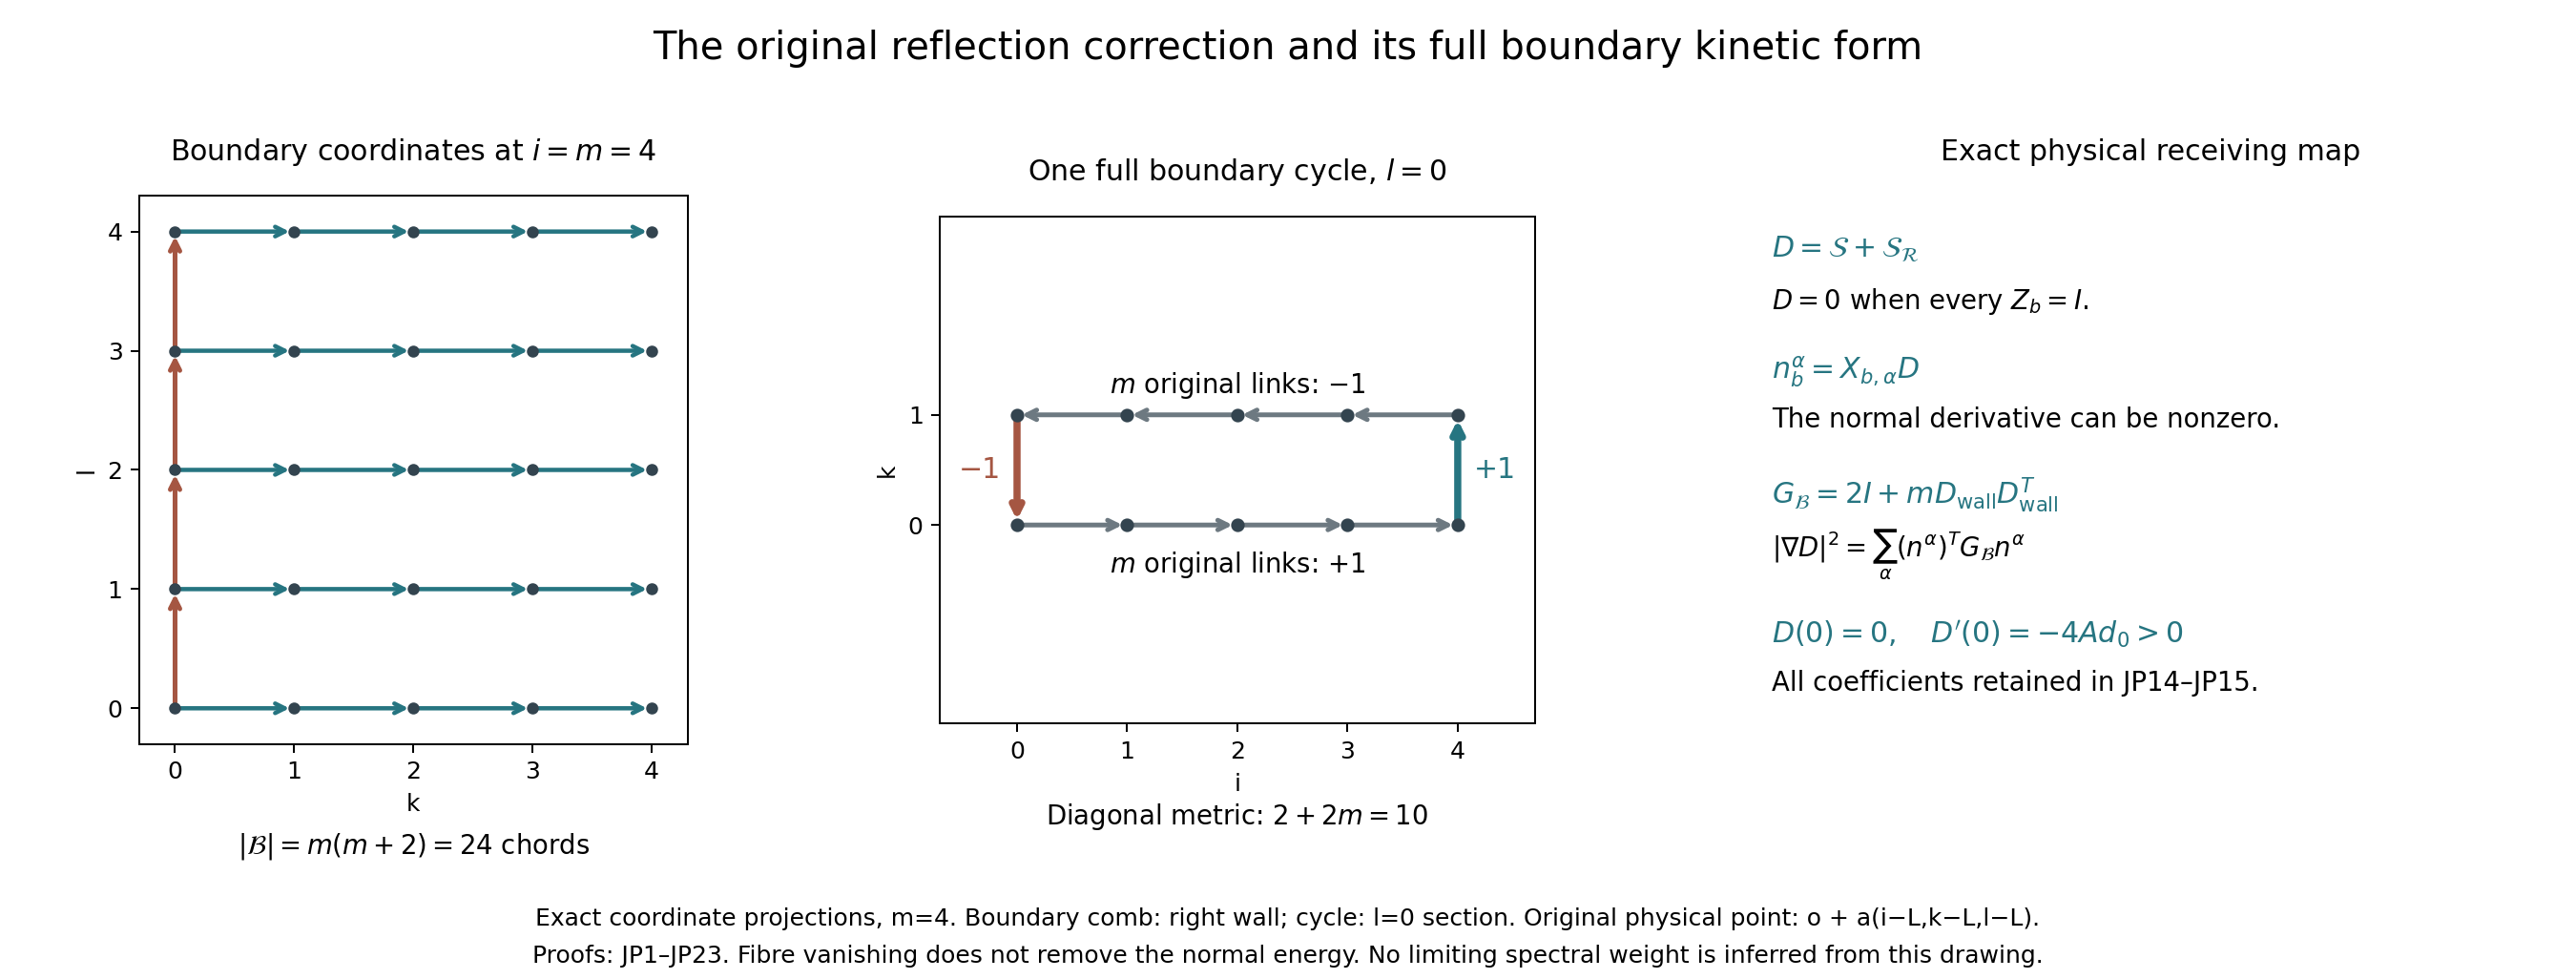
\includegraphics[width=\linewidth,height=.72\textheight,keepaspectratio]{BOUNDARY_REFLECTION.png}\caption{Boundary comb, complete original cycle and normal kinetic map. Exact coordinate sections at m=4; proof JP1–JP23.}\end{figure}

\begin{figure}[htbp]\centering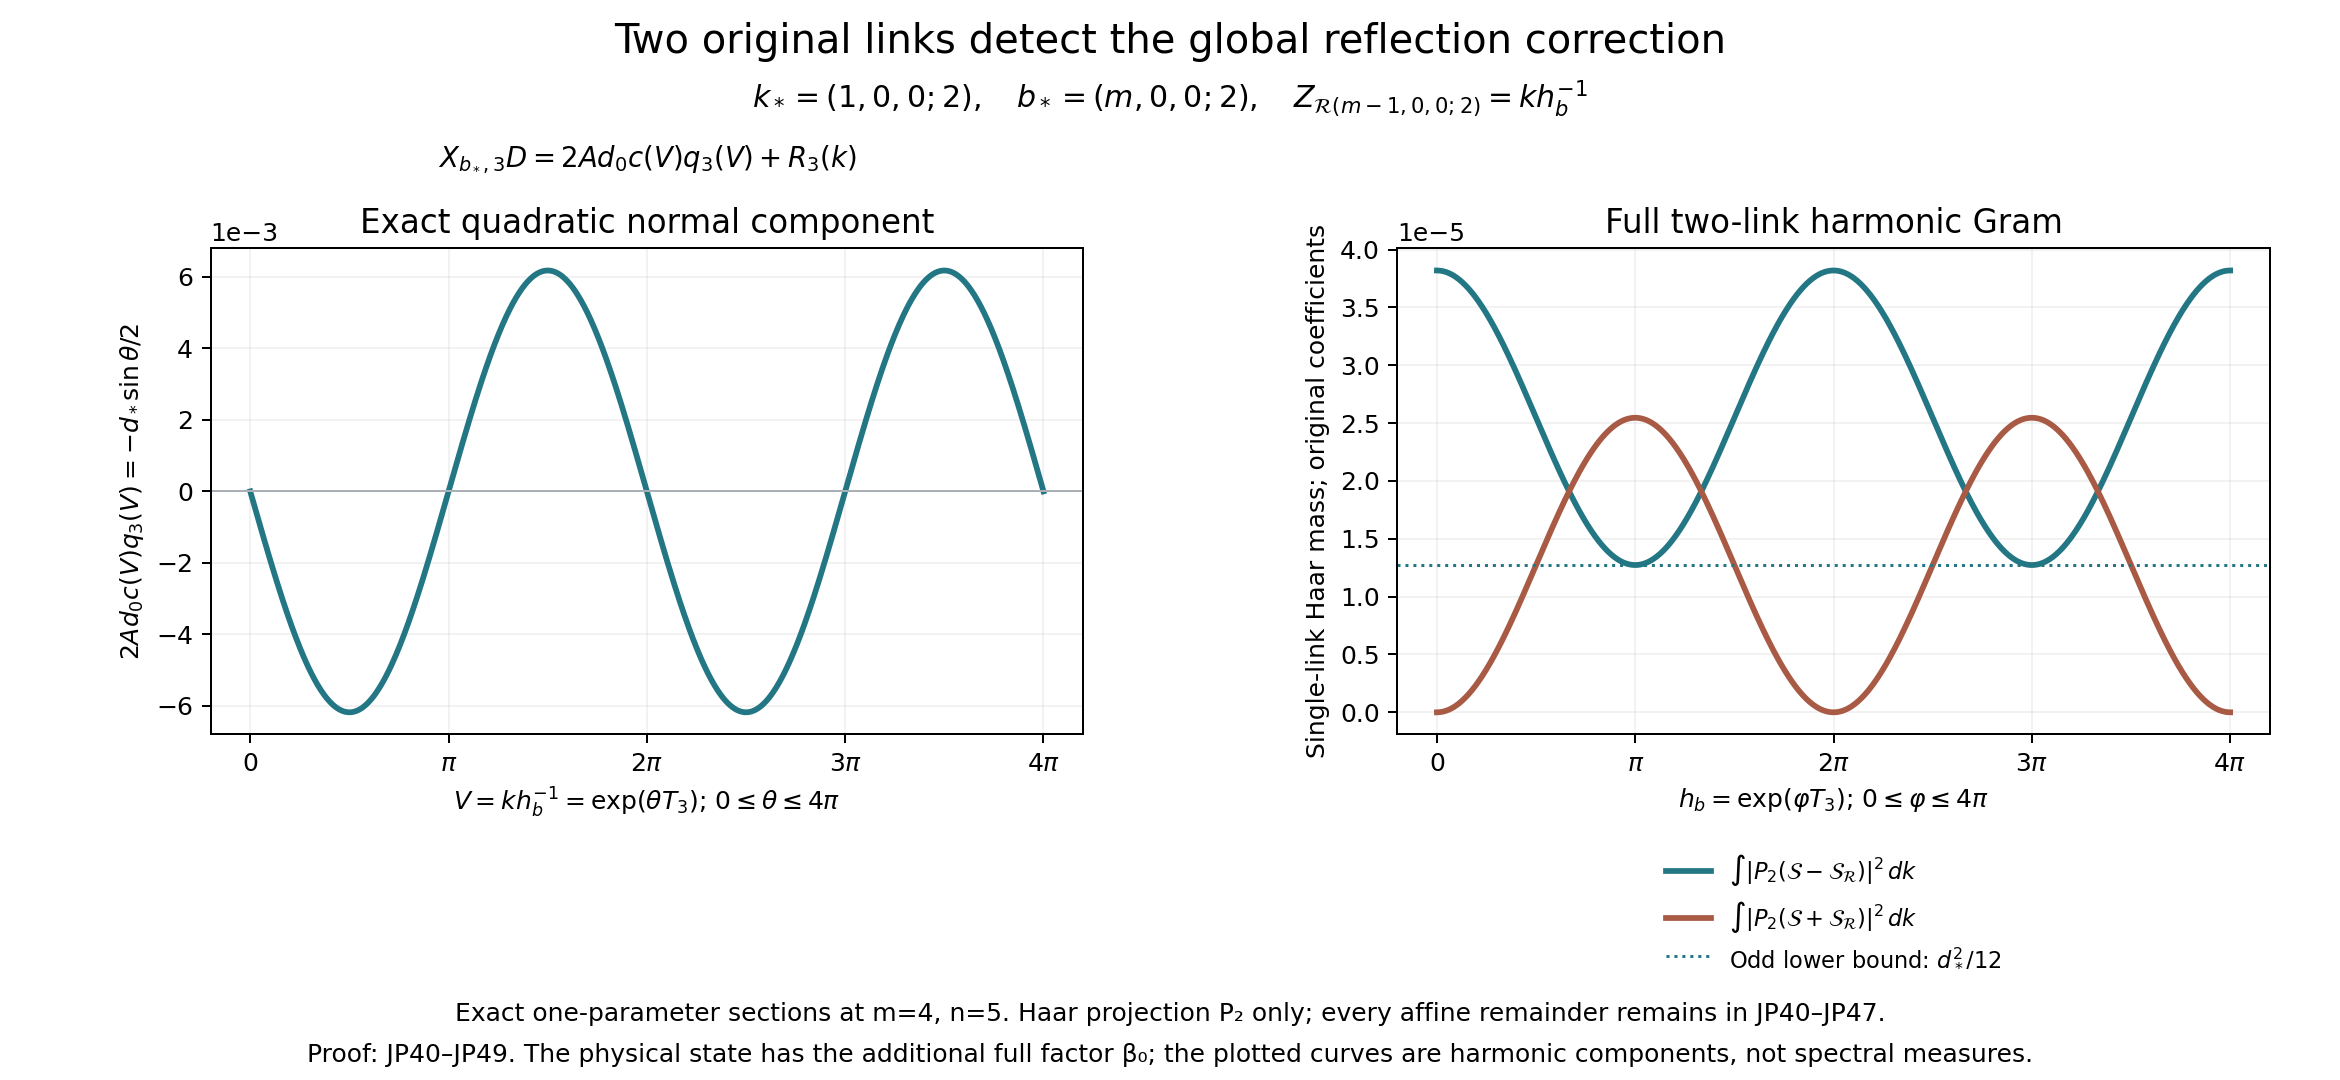
\includegraphics[width=\linewidth,height=.72\textheight,keepaspectratio]{TWO_LINK_HARMONICS.png}\caption{Two original links and their complete quadratic harmonic components. Exact sections at m=4; affine remainders and the physical factor beta0 remain in JP40–JP49.}\end{figure}

\begin{figure}[htbp]\centering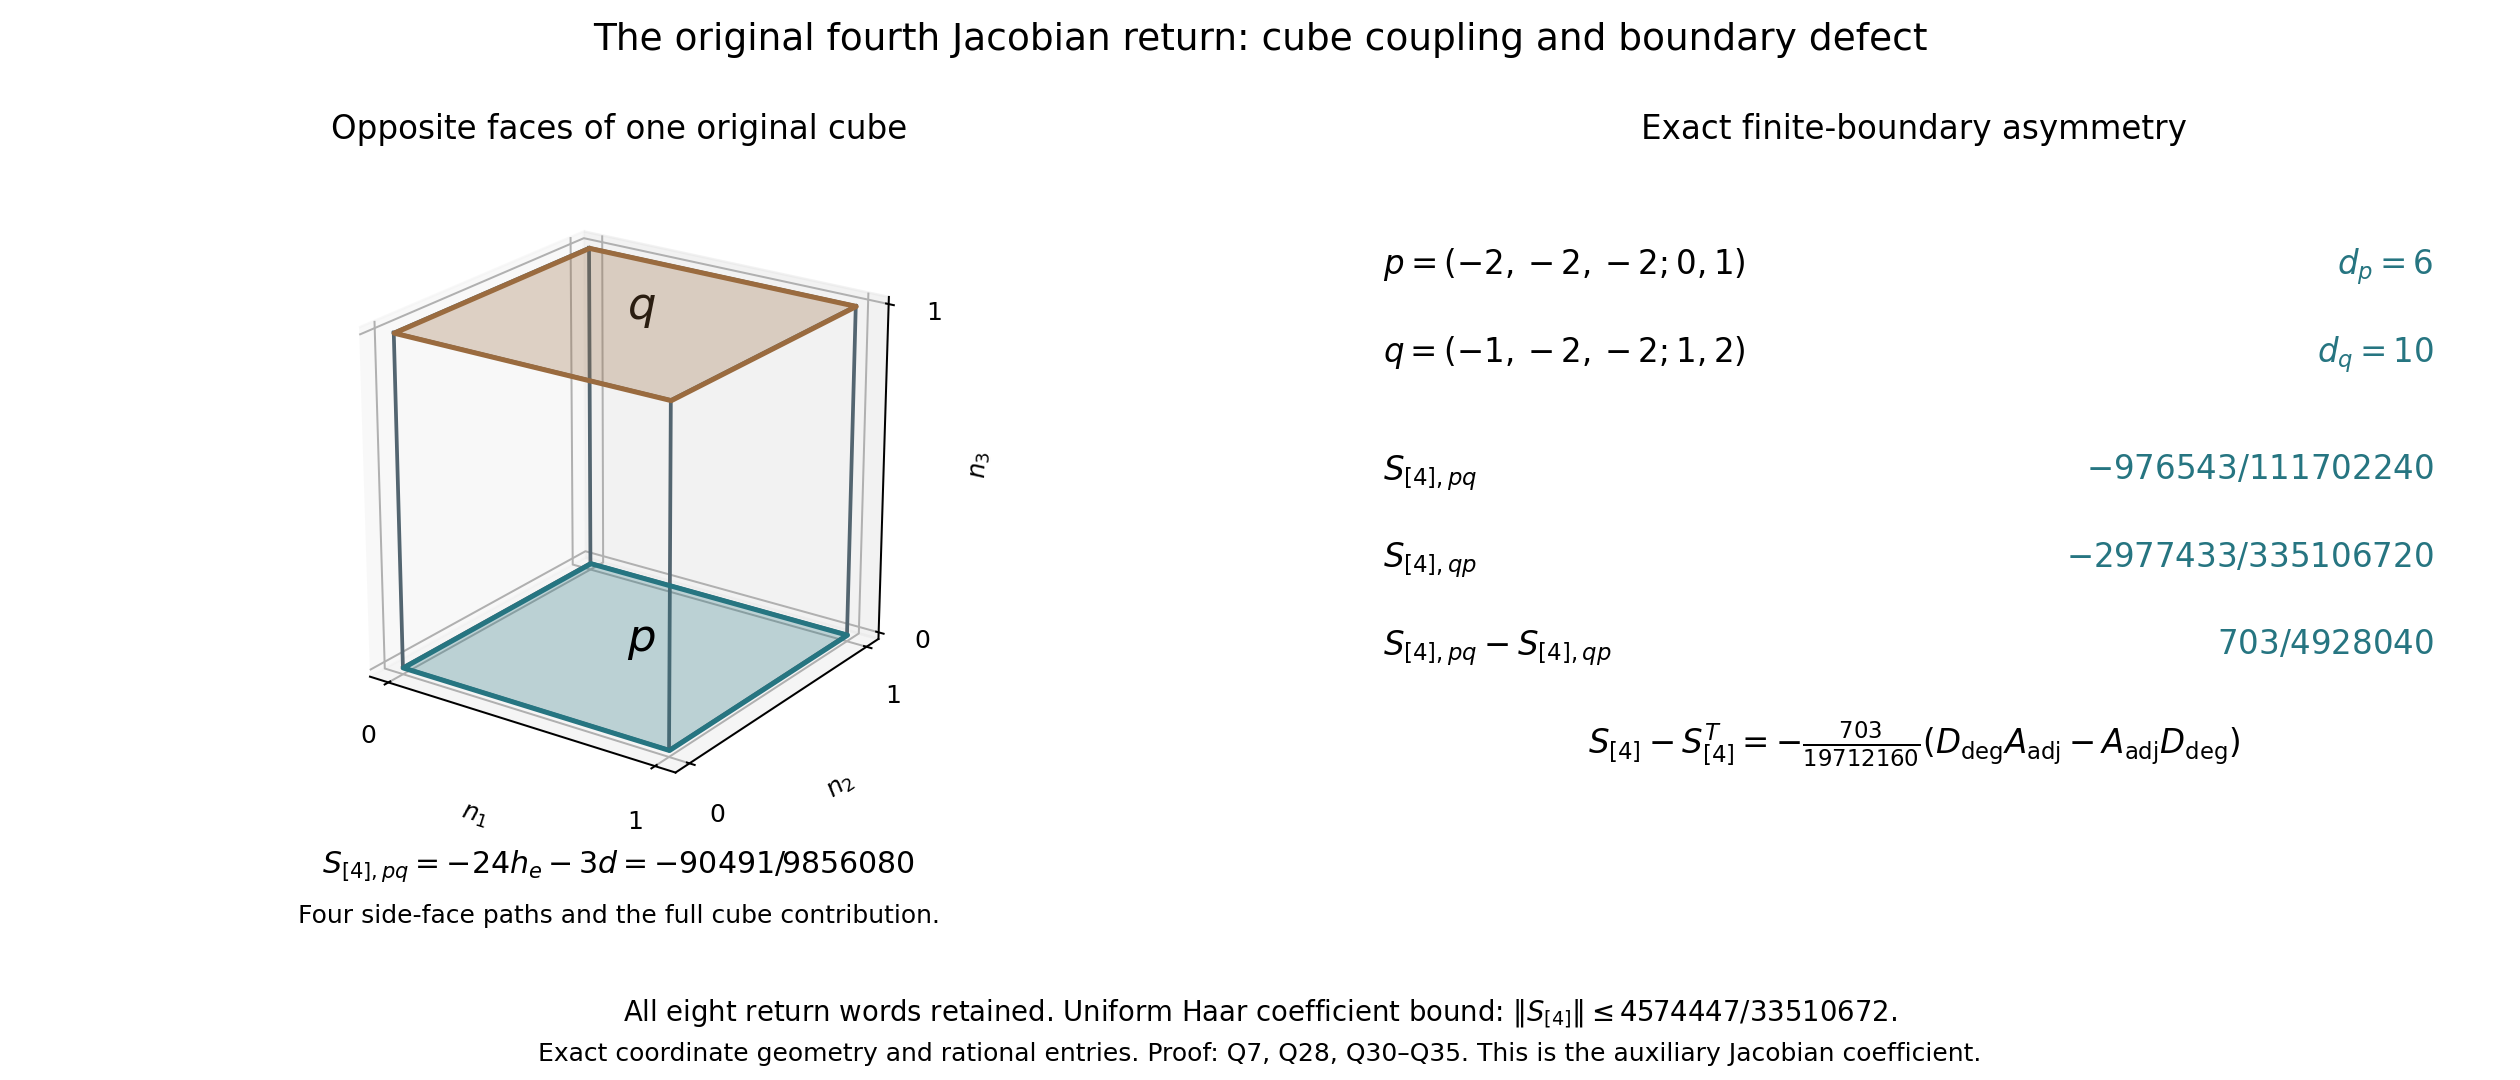
\includegraphics[width=\linewidth,height=.72\textheight,keepaspectratio]{FOURTH_SCHUR.png}\caption{Opposite faces of one original cube and the finite-boundary skew matrix. Exact rational entries and coefficient bound; proof Q7, Q28, Q30–Q35.}\end{figure}

These images depict the exact objects, coordinate sections and proved coefficients in the accompanying complete proofs. They do not depict a constructed continuum quantum state or a limiting spectral measure. The three Python sources reproduce the rendered figures.
\clearpage
\section*{The exact physical source inverse at every finite real source}

11 October 2026. All statements below concern the original finite open cubic box. The Hamiltonian, Haar probability measure, vertex constraints, edge metric, face words, support relations and scalar energy are retained. The final estimates are evaluated on the original joint path. No closing physical gap or continuum Yang–Mills theorem is claimed.

The receiving definitions are Q1–Q5 and Q42–Q47 in \href{https://github.com/KokunoYumeto/yang-mills-interacting-workbench/blob/44548a167319316397e6874d8b2fc8f1d3491137/yang-mills/continuations/20261011-central-signs-shrinking-window/fourth_return/FOURTH_SCHUR_COEFFICIENT.md}{the complete fourth Schur coefficient}. The original labelled space and bilinear map are \href{https://github.com/KokunoYumeto/yang-mills-interacting-workbench/blob/fa79faff2cd697e16cfa3a7953f36810c22c8922/yang-mills/continuations/20260915-gauge-native-band/RESEARCH_NOTE.md}{G1–G23}. The local score calculation used below is reproduced, including its extension to signed sources, from \href{https://github.com/KokunoYumeto/yang-mills-interacting-workbench/blob/7d5681ed53835433a5fb72d880b6292832f2efbf/yang-mills/continuations/20260930-s6-ns-moment-map-bridge/sources/spatial/spatial_continuum.tex#L1414}{Spatial continuum, Section 10.1, equations (77)–(78)}. These are programme sources. No novelty or exhaustive-literature claim is made for elliptic perturbation theory, the ground-state transform, susceptibility, or convex duality. The existing canonical literature indexes were queried before this derivation; their hits are routing records only.

\subsection*{1. Original objects, vacuum and all Sobolev domains}

Let \(L\ge2\) be an integer. Keep
\[
 V_L=\{-L,\ldots,L\}^3,\quad
 E_L=\{(n,i):n,n+e_i\in V_L\},\quad
 \mathcal P_L=\{(n;i,j):i<j,\ n,n+e_i,n+e_j,n+e_i+e_j\in V_L\}.
 \tag{GPR1}
\]
Write \(N=|E_L|=3(2L)(2L+1)^2\), \(M=|\mathcal P_L|=3(2L)^2(2L+1)\), and \(Q_L=SU(2)^{E_L}\), with product Haar probability \(dU\). On the original positive edges set
\[
\begin{split}
 W_{(n;i,j)}(U)&=\operatorname{Tr}[U_i(n)U_j(n+e_i)U_i(n+e_j)^{-1}U_j(n)^{-1}],\\
 T_\alpha&=-i\sigma_\alpha/2,\quad
 X_{e,\alpha}f=\left.\frac d{dt}f(\ldots,e^{tT_\alpha}U_e,\ldots)\right|_{t=0},\\
 K&=-\sum_{e,\alpha}X_{e,\alpha}^2,\qquad
 \Gamma(f,h)=\sum_{e,\alpha}(X_{e,\alpha}f)(X_{e,\alpha}h),\\
 H(x)&=\kappa K+V_x,\qquad
 V_x=\kappa\sum_{p\in\mathcal P_L}x_p(2-W_p),\quad
 x\in\mathbb R^M,\quad\kappa>0.
\end{split}\tag{GPR2}
\]
For complex functions the energy integrand is \(\Gamma(\bar f,f)\). Each original vertex, including every boundary vertex, acts by \(U_e\mapsto q_sU_eq_t^{-1}\). Its Haar average is the orthogonal projection \(\Pi\). A function or distribution is physical when \(\Pi f=f\). The action commutes with \(K\), \(H(x)\), and every Sobolev operator used below. The displayed potential contains its full scalar \(2\kappa\sum_p x_p\).

Define the Sobolev scale by
\[
 H^s(Q_L)=\{f:(I+K)^{s/2}f\in L^2(dU)\},\quad
 \|f\|_{H^s}=\|(I+K)^{s/2}f\|_2,
\quad
 H^s_{\rm ph,0}=\{f\in H^s:\Pi f=f,\ \langle f,1\rangle=0\}.
 \tag{GPR3}
\]
For negative \(s\) this is the distribution completion and the mean is its distribution pairing with the smooth function \(1\). The product-spin eigenvalues of \(K\) are \(c(j)=\sum_ej_e(j_e+1)\), with multiplicity bounded by \(\prod_e(2j_e+1)^2\). This gives the compact inclusions \(H^{s+1}\hookrightarrow H^s\): cut off the finitely many blocks with \(c(j)\le R\), and the remaining inclusion norm is at most \((1+R)^{-1/2}\). Smooth multiplication acts boundedly on every \(H^s\), and each \(X_{e,\alpha}\) maps \(H^s\to H^{s-1}\); for integer \(s\ge0\) these follow from the product rule and the Casimir derivative bounds, for negative integers from duality, and for intervening real indices from the spectral interpolation inequality. Thus all operator mappings used below have fixed, specified domains.

Every nonconstant physical product-spin block has \(c(j)\ge3\). Indeed, a degree-one vertex of its active edge graph would require a nonzero invariant in one nontrivial irreducible \(SU(2)\) representation. No such invariant exists. A nonempty finite graph without degree-one vertices contains a cycle. The original cubic graph has no cycle shorter than four, and every nontrivial edge spin contributes at least \(3/4\). A fundamental face trace attains \(3\). The complete physical Peter–Weyl decomposition therefore proves
\[
 K:H^s_{\rm ph,0}\longrightarrow H^{s-2}_{\rm ph,0}
 \text{ is an isomorphism},\qquad
 \|K^{-1}\|_{H^{s-2}\to H^s}\le4/3,
 \qquad KW_p=3W_p.
 \tag{GPR4}
\]
The factor \(4/3\) is \((1+c)/c\le4/3\). Distinct face traces are orthogonal and each has norm one: integrating a link present in only one face gives zero, and a face holonomy is Haar, with fundamental character square integral one. In particular \(\int W_p=0\).

The potential is real, smooth and bounded for every finite real \(x\), so \(H(x)\) is self-adjoint on \(H^2\), has form domain \(H^1\), and has compact resolvent. A lowest Rayleigh minimizer exists by compactness, and replacing it by its modulus cannot increase its kinetic form. The eigen-equation and elliptic regularity make that nonnegative minimizer smooth. The strong maximum principle for a bounded zeroth-order coefficient makes it strictly positive on the connected product. Denote it by \(\psi_x\), with \(\int\psi_x^2dU=1\), and its eigenvalue by \(E(x)\). One can see the required regularity directly by rewriting \(K\psi=(E-V_x)\psi/\kappa\) and successively applying the spectral inverse of \(I+K\); smooth multiplication preserves each successive Sobolev space.

For smooth \(F\), the product rule \(K(fh)=fKh+hKf-2\Gamma(f,h)\), the full vacuum equation, and integration by parts give
\[
 \langle\psi_xF,(H(x)-E(x))\psi_xF\rangle
 =\kappa\int\psi_x^2\Gamma(\bar F,F)dU.
 \tag{GPR5}
\]
Division by the positive smooth \(\psi_x\) preserves \(H^1\). If a second ground vector is divided by \(\psi_x\), (GPR5) makes all its first derivatives zero; connectedness makes it constant. Thus the ground eigenspace is one-dimensional. Every vertex gauge action fixes the positive unit vector, since it preserves \(H(x)\), positivity and norm. Consequently \(\psi_x\) is physical. This also proves that the physical and full ground energies coincide. At this fixed finite source the next physical eigenvalue is separated from \(E(x)\); write this actual positive difference as \(\delta(x)\).

Put
\[
 \rho_x=\psi_x^2,\quad d\mu_x=\rho_xdU,\quad
 P_Hf=\int f\,dU,\quad Q_H=I-P_H,\quad
 v_x=\log\psi_x-P_H\log\psi_x,\quad
 c_x=P_H\log\psi_x=-\tfrac12\log\int e^{2v_x}dU.
 \tag{GPR6}
\]
No normalization scalar is omitted. The full logarithmic equation and its Haar mean are
\[
 Kv_x=\sum_p x_pW_p+\Gamma(v_x,v_x)-\int\Gamma(v_x,v_x)dU,
 \qquad
 E(x)=2\kappa\sum_p x_p-\kappa\int\Gamma(v_x,v_x)dU.
 \tag{GPR7}
\]
They follow by dividing \(H\psi=E\psi\) by \(\psi=e^{v+c}\), using \(K(e^v)=e^v(Kv-\Gamma(v,v))\), and taking the original Haar integral.

\subsection*{2. The full inverse and its source dependence}

Multiplication \(U_xF=\psi_xF\) is a unitary map from \(L^2(\mu_x)_{\rm ph}\) onto \(L^2(dU)_{\rm ph}\). Its operator and form domains are \(H^2_{\rm ph}\) and \(H^1_{\rm ph}\), respectively, under the unchanged coordinate Sobolev scale. The exact conjugate is
\[
 \mathcal L_x=K-2\Gamma(v_x,\cdot)
 =\kappa^{-1}\psi_x^{-1}(H(x)-E(x))\psi_x,
 \quad
 \int\mathcal L_xh\,d\mu_x=0.
 \tag{GPR8}
\]
The last identity holds first for smooth \(h\) by integration by parts and then for distributions by duality with the smooth density. In particular the only physical distributional solutions of \(\mathcal L_xh=0\) are constants: elliptic bootstrapping makes them smooth and (GPR5) applies.

Define on every real Sobolev index
\[
 \mathscr L_x
 =I-2K^{-1}Q_H\Gamma(v_x,\cdot)
 =K^{-1}Q_H\mathcal L_x:
 H^s_{\rm ph,0}\longrightarrow H^s_{\rm ph,0}.
 \tag{GPR9}
\]
The perturbation of the identity maps \(H^s\to H^{s+1}\), because its drift is first order and \(K^{-1}Q_H\) gains two derivatives. It is therefore compact on \(H^s_{\rm ph,0}\). If \(\mathscr L_xh=0\), repeated use of the same one-derivative gain makes \(h\) smooth. The equation says \(\mathcal L_xh=b\) for a constant \(b\). Its \(\mu_x\) mean gives \(b=0\). Equation (GPR5) makes \(h\) constant, and its Haar mean is zero. Hence \(h=0\). An identity minus a compact operator has index zero; its trivial kernel therefore gives a bounded bijection in (GPR9). This argument proves invertibility at every finite real source, with no small-source assumption.

Here is the complete formula. Let \(A_x=H(x)-E(x)\) and let \(A_x^\dagger\) be its inverse on \(\psi_x^\perp\cap L^2(dU)_{\rm ph}\), extended to annihilate \(\psi_x\). Then
\[
 \boxed{
 \mathscr L_x^{-1}f
 =Q_H\,\kappa\psi_x^{-1}A_x^\dagger\psi_x
       [Kf-\mu_x(Kf)] .}
 \tag{GPR10}
\]
For \(f\in H^2_{\rm ph,0}\), the bracket is in \(L^2\), and \(\psi_x[Kf-\mu_x(Kf)]\perp\psi_x\). Applying (GPR8) proves that the expression before \(Q_H\) solves \(\mathcal L_xh=Kf-\mu_x(Kf)\). Subtracting its Haar mean does not change that equation. Applying \(K^{-1}Q_H\) proves (GPR10). Conversely any solution of \(\mathscr L_xh=f\) must have \(\mathcal L_xh=Kf+b\); its \(\mu_x\) mean forces the specific scalar \(b=-\mu_x(Kf)\). Thus the two distinct means in (GPR10) are both necessary.

For arbitrary real \(s\), interpret \(\mu_x(Kf)=\langle Kf,\rho_x\rangle=\langle f,K\rho_x\rangle\). Extend \(A_x^\dagger:H^{s-2}_{\rm ph}\to H^s_{\rm ph}\) by its elliptic inverse with the rank-one vacuum projection removed. To check this extension without assuming it, apply (GPR9) to solve \(\mathcal L_xh=g-\mu_x(g)\) for \(g\in H^{s-2}_{\rm ph}\), setting \(f=K^{-1}Q_Hg\); the missing constant is fixed by the same mean identity. Multiplication by \(\psi_x\) then solves the distributional \(A_x\) equation, and subtraction of the \(\psi_x\) component fixes its unique inverse. This agrees with the \(L^2\) spectral inverse on the intersection of the domains by uniqueness. Consequently (GPR10) is a bounded inverse with exactly the claimed domains at every \(s\in\mathbb R\).

All of these maps depend real analytically on \(x\in\mathbb R^M\), locally as maps in their stated bounded-operator norms. At a fixed \(x_0\), take a circle enclosing only \(E(x_0)\). The bounded potential difference has norm at most \(4\kappa\sum_p|x_p-x_{0,p}|\); a sufficiently small complex neighbourhood makes the resolvent Neumann expansion uniform on that circle. Its contour integral is an analytic rank-one projection. Apply it to \(\psi_{x_0}\), and divide by the analytic square root of its bilinear integral \(\int\phi_x^2dU\), choosing the branch equal to one at \(x_0\). On real nearby sources this is the positive unit vacuum. The resolvent equation and successive Sobolev estimates make this dependence analytic in every \(H^r\). Sobolev embedding at \(r>3N/2+k\) gives it in \(C^k\). Positivity at \(x_0\) and the convergent power series of the logarithm give analytic \(v_x\in C^k\) on a smaller neighbourhood. Thus (GPR9) is analytic on \(H^s\); the ordinary local Neumann expansion around its already proved inverse proves analytic \(\mathscr L_x^{-1}\). Unique positive phases agree on overlaps. This is global real analytic dependence, meaning a compatible local analytic family at every real point; it does not assert a single complex power-series disk reaching all real sources.

\subsection*{3. The exact comparison with every original support label}

For \(t\ge0\) let \(Y_t\) be the physical zero-Haar-mean Fourier space with
\[
 f=\sum_{j\ne0}\operatorname{Tr}(A_j\pi_j),\qquad
 \|f\|_{Y_t}=\sum_{j\ne0}c(j)^t\|A_j\|_1.
 \tag{GPR11}
\]
The original labelled Banach space \(\mathfrak B\) retains all nonempty edge labels \(S\subseteq E_L\) and all coefficients whose active spin support is contained in \(S\), including strict containment. Its norm and assembly are
\[
 \|F\|_{\rm loc}=\max_{e\in E_L}\sum_{S\ni e}\sum_{j\ne0}c(j)\|A_{S,j}\|_1,
 \quad
 \mathsf aF=\sum_j\operatorname{Tr}\!\left[\Big(\sum_{S\supseteq\operatorname{supp}j}A_{S,j}\Big)\pi_j\right].
 \tag{GPR12}
\]
Summing the anchor norms counts each original label at least once, so
\[
 \|\mathsf aF\|_{Y_1}\le N\|F\|_{\rm loc},\qquad
 \|\mathsf aF\|_{H^2}\le\tfrac43N\|F\|_{\rm loc}.
 \tag{GPR13}
\]
For the second inequality use the triangle inequality on the \(L^2\) functions and \((1+c)/c\le4/3\). Absolute coefficient convergence also gives \(\mathsf aF\in C^2\): zeroth coefficients have bound \(c/3\), first derivatives have \(j_e\le\sqrt c\), and each ordered second derivative has \(j_ej_f\le c\), including the case \(e=f\). Every component converges uniformly with these derivatives.

There is a bounded section \(\iota:Y_1\to\mathfrak B\): place each coefficient in the existing full original edge label \(E_L\). It has \(\|\iota f\|_{\rm loc}=\|f\|_{Y_1}\) and \(\mathsf a\iota=I\). This is a comparison map; it does not replace any existing support label. The relation \(F-\iota\mathsf aF\) is kept in \(\ker\mathsf a\), coefficient by coefficient. The original quotient is exactly
\[
 \overline{\mathsf a}:\mathfrak B/\ker\mathsf a\xrightarrow{\cong}Y_1,
 \quad
 \|[F]\|_{\rm quotient}\le\|\overline{\mathsf a}[F]\|_{Y_1}
 \le N\|[F]\|_{\rm quotient}.
 \tag{GPR14}
\]
The first inequality uses the explicit representative \(\iota\mathsf aF\); the second follows from (GPR13) and the infimum over representatives. Both constants depend on the original finite volume as displayed.

The original union-label bilinear map is
\[
 \mathcal B(F,G)_S=K^{-1}Q_H
       \sum_{S_1\cup S_2=S}\Gamma(F_{S_1},G_{S_2}).
\]
It obeys the exact intertwining
\[
 \mathsf a\mathcal B(F,G)=K^{-1}Q_H\Gamma(\mathsf aF,\mathsf aG),
 \qquad
 \mathsf a(I-2\mathcal B(V,\cdot))
 =\mathscr L_x\mathsf a\quad\text{when }\mathsf aV=v_x.
 \tag{GPR15}
\]
First verify this on finite coefficient families, where it is just the displayed sum over every original union. Then use the original G13 bilinear bound and (GPR13) to pass to the Banach completion and \(H^2\), respectively. The assembly kernel is invariant, since the right side vanishes on it.

In particular, in the previously proved labelled small-source disk, the original Neumann inverse and the physical inverse satisfy
\[
 \mathsf a(I-2\mathcal B(V(x),\cdot))^{-1}
 =\mathscr L_x^{-1}\mathsf a.
 \tag{GPR16}
\]
Both sides solve the same physical equation, and (GPR9) gives uniqueness. The same equation holds for the quotient inverse. This proves the inclusion and comparison, without extending the radius of convergence of the old labelled Taylor series.

One can prove more for the original finite-volume quotient, independently of that series. Smooth \(v_x\) belongs to every \(Y_t\). Indeed, trace-norm/Hilbert–Schmidt duality and Peter–Weyl Plancherel give
\[
 \sum_jc(j)^t\|A_j\|_1
 \le\left(\sum_j d_j^2\frac{c(j)^{2t}}{(1+c(j))^r}\right)^{1/2}\|v_x\|_{H^r},
 \tag{GPR17}
\]
where \(d_j=\prod_e(2j_e+1)\). The sum is finite when \(r>2t+3N/2\), by comparison with the product-spin lattice sum in dimension \(3N\). The missing constant coefficient of \(v_x\) is zero.

The original tensor-product trace-norm estimate and spin-generator norm give, for the drift coefficient product, a bound \(3\sum_e j_ek_e\le3\sqrt{c(j)c(k)}\). Any output spin has \(c(\ell)\le2(c(j)+c(k))\), since \(\ell_e\le j_e+k_e\) and \((j_e+k_e)(j_e+k_e+1)\le2[j_e(j_e+1)+k_e(k_e+1)]\). Keeping all three colour derivatives therefore proves
\[
 \|K^{-1}Q_H\Gamma(v_x,h)\|_{Y_{3/2}}
 \le3\sqrt2\big(\|v_x\|_{Y_1}\|h\|_{Y_{1/2}}
                  +\|v_x\|_{Y_{1/2}}\|h\|_{Y_1}\big).
 \tag{GPR18}
\]
The inverse Casimir cancels one power of the output weight. The remaining square root is bounded by \(\sqrt2(\sqrt{c(j)}+\sqrt{c(k)})\); this gives the two terms and the constant in (GPR18). Since \(\|h\|_{Y_{1/2}}\le3^{-1/2}\|h\|_{Y_1}\), this is a bounded map \(Y_1\to Y_{3/2}\). The inclusion \(Y_{3/2}\to Y_1\) is compact: only finitely many finite-dimensional matrix blocks lie below a Casimir cutoff, and the remaining inclusion norm is at most \(R^{-1/2}\). Hence \(\mathscr L_x\) is identity minus a compact operator on \(Y_1\). Its kernel embeds in the already trivial \(H^2\) kernel. The index-zero argument proves a bounded \(Y_1\) inverse at every finite real source. Formula (GPR10) and uniqueness identify it exactly with the Sobolev inverse on \(Y_1\).

Thus (GPR14) transports this independently proved inverse to the original assembly quotient at all finite real sources. The source \(v_x\) and this inverse are real analytic in that quotient, by (GPR17) and the Sobolev analytic result. This does not assert an inverse on the unquotiented relation kernel, a volume-uniform quotient norm, or continuation of the old Taylor series beyond its established disk. Every original relation remains present in (GPR12)–(GPR16).

\subsection*{4. Strict physical response, observation and global source coordinates}

Set \(m_p(x)=\mu_x(W_p)\), \(z_q=\partial_{x_q}v_x\), and \(Z_q=z_q-\mu_x(z_q)\). Differentiating the full normalization and eigen-equation gives
\[
 \partial_{x_q}\psi_x=\psi_xZ_q,\qquad
 \partial_{x_q}E(x)=\kappa(2-m_q),\qquad
 A_x(\psi_xZ_q)=\kappa(W_q-m_q)\psi_x,
 \qquad \mathscr L_xz_q=W_q/3.
 \tag{GPR19}
\]
For the last equation differentiate (GPR7), apply \(K^{-1}Q_H\), and use \(KW_q=3W_q\). All derivatives exist by Section 2.

With \(r_p=(W_p-m_p)\psi_x\), the original physical response is
\[
 \begin{split}
 R^{\rm phys}_{pq}(x)
 &=\kappa\langle r_p,A_x^\dagger r_q\rangle_{L^2(dU)}
 =\mu_x[(W_p-m_p)z_q],\\
 \partial_{x_q}m_p&=2R^{\rm phys}_{pq},\qquad
 \partial_{x_p}\partial_{x_q}E=-2\kappa R^{\rm phys}_{pq}.
 \end{split}\tag{GPR20}
\]
These identities hold for every finite real source. The matrix is real symmetric and strictly positive definite. To prove strictness, let \(a\in\mathbb R^M\) be nonzero and \(F_a=\sum_pa_pW_p\). The source vector \(r_a=(F_a-\mu_xF_a)\psi_x\) cannot vanish: positivity of \(\psi_x\) and continuity would make \(F_a\) constant everywhere, whereas its Haar mean is zero and its Haar squared norm is \(\sum_pa_p^2>0\). The positive inverse of \(A_x\) on \(\psi_x^\perp\) therefore has strictly positive quadratic form at \(r_a\). The same conclusion for complex coefficient vectors follows by real and imaginary parts.

On \(H^s_{\rm ph,0}\), including distributional \(s\), retain the exact finite-rank observation
\[
 \mathcal O_{\rho_x}h
 =\sum_pW_p\{\langle h,\rho_xW_p\rangle
                       -m_p\langle h,\rho_x\rangle\},\qquad
 Ph=\sum_pW_p\langle h,W_p\rangle.
 \tag{GPR21}
\]
All paired functions are smooth. With the original Haar-orthonormal face basis, the global identity is
\[
 \boxed{3R^{\rm phys}(x)=\mathcal O_{\rho_x}\mathscr L_x^{-1}P.}
 \tag{GPR22}
\]
In the old labelled disk, (GPR16) identifies it with Q46 after assembly. The exact Q47 comparison with the fifth reference remains valid wherever its own inverse exists, with every operator understood through this inclusion. Its two corrections, the observation change and the higher-source resolvent term, remain necessary. At \(x=0\), \(\rho=1\), \(\mathscr L=I\), \(\mathcal O_\rho=P\), and \(R^{\rm phys}=I_M/3\).

There is also a complete global description of the expectation coordinates. Let
\[
 \mathcal C_L=\operatorname{conv}\{(W_p(U))_{p\in\mathcal P_L}:U\in Q_L\}\subset\mathbb R^M,
 \qquad \Lambda(x)=2\sum_px_p-E(x)/\kappa.
 \tag{GPR23}
\]
The convex hull is compact and has nonempty interior. If it were contained in an affine hyperplane, a nonzero \(a\) would make \(F_a\) constant, contrary to the Haar calculation above. Variationally, \(\Lambda(x)\) is the largest eigenvalue of \(-K+\sum_px_pW_p\); the equality retains rather than discards the scalar in \(H(x)\). By (GPR20), \(\nabla\Lambda=m(x)\) and \(D^2\Lambda=2R^{\rm phys}>0\).

For every finite \(x\), \(m(x)\in\operatorname{int}\mathcal C_L\). Otherwise a supporting hyperplane would give a nonconstant \(F_a\le h_{\mathcal C_L}(a)\) whose positive-density integral equals its maximum. Its continuous nonnegative deficit would then vanish everywhere, a contradiction. Strict Hessian positivity makes \(m\) injective, since for \(x\ne y\)
\[
 (x-y)\cdot(m(x)-m(y))
 =2\int_0^1(x-y)^tR^{\rm phys}(y+t(x-y))(x-y)\,dt>0.
 \tag{GPR24}
\]
It is onto this interior as well. Fix \(b\in\operatorname{int}\mathcal C_L\), and take \(\varepsilon>0\) with \(b+\varepsilon\overline B\subset\mathcal C_L\). For each unit vector \(u\), choose a configuration where \(F_u\) attains its maximum and a nonzero smooth bump supported where \(F_u>h_{\mathcal C_L}(u)-\varepsilon/4\). Its unit Rayleigh quotient for \(-K+tF_u\) is at least \(t[h_{\mathcal C_L}(u)-\varepsilon/4]-C_u\), with finite \(C_u=\int\Gamma(\bar\phi_u,\phi_u)dU\). Because \(\|W(U)\|\le2\sqrt M\), both the support function and these trial expectations are \(2\sqrt M\)-Lipschitz in \(u\). Finitely many neighbourhoods of these \(u\)'s cover the unit sphere. Their finite maximum kinetic cost \(C_\varepsilon\) gives, for every unit \(u\) and \(t\ge0\),
\[
 \Lambda(tu)-t\,u\cdot b\ge t\varepsilon/2-C_\varepsilon.
 \tag{GPR25}
\]
The variational inequality is valid in the full Hilbert space, whose largest eigenvalue here equals the physical one by ground positivity. Thus no gauge-variant trial is declared to be a physical state. Equation (GPR25) proves coercivity. The smooth strictly convex function \(\Lambda(x)-x\cdot b\) has a unique minimizer, and its derivative there is \(m(x)-b=0\). The analytic inverse-function theorem and uniqueness join the local inverses. Therefore
\[
 \boxed{m:\mathbb R^M\xrightarrow{\text{real analytic diffeomorphism}}
                   \operatorname{int}\mathcal C_L,\qquad
 D(m^{-1})=(2R^{\rm phys})^{-1}.}
 \tag{GPR26}
\]
This is a result about the actual finite-box ground state and the original joint Wilson image. It supplies no uniform limit of these convex bodies or inverses as \(L\to\infty\).

\subsection*{5. Explicit bounds, including a polynomial local bound}

Set
\[
 s_e(x)=\sum_{p:e\in\partial p}|x_p|,\quad
 S(x)=2\left(\sum_es_e(x)^2\right)^{1/2},\quad
 \Omega(x)=8\pi\sum_es_e(x)=32\pi\sum_p|x_p|.
 \tag{GPR27}
\]
In the metric where the original \(X_{e,\alpha}\) are orthonormal, each factor is a radius-two three-sphere, with Ricci tensor one half its metric and diameter \(2\pi\). Write \(u=\log\psi_x\), \(\Delta=-K\), and \(w_e=|\nabla_eu|^2\). The full vacuum equation says \(\Delta u+|\nabla u|^2=(V_x-E)/\kappa\). Differentiating it and the squared partial gradient gives the complete product Bochner identity
\[
 (\Delta+2\nabla u\cdot\nabla)w_e
 =2\sum_f|\nabla_f\nabla_eu|_{\rm HS}^2+w_e
       +2\kappa^{-1}\langle\nabla_eu,\nabla_eV_x\rangle.
 \tag{GPR28}
\]
The factor-\(e\) curvature contributes \(2\operatorname{Ric}_e=w_e\); mixed factors have zero curvature. The derivative of \(-|\nabla u|^2\) cancels the displayed drift, retaining every mixed Hessian. For an original face containing \(e\), bi-invariance and inversion reduce its trace gradient to that of \(2u_0\) on the radius-two sphere, with squared norm \(1-u_0^2\le1\). Consequently \(\|\nabla_eV_x\|_\infty\le\kappa s_e\). At the maximum of \(w_e\), (GPR28) gives \(0\ge w_e-2s_e\sqrt{w_e}\). Thus
\[
 \|\nabla_e\log\psi_x\|_\infty\le2s_e,
 \quad\|\nabla_e\log\rho_x\|_\infty\le4s_e,
 \quad\|\nabla v_x\|_\infty\le S,
 \quad\frac{\max\rho_x}{\min\rho_x}\le e^\Omega.
 \tag{GPR29}
\]
The last inequality follows by moving each original link along a shortest geodesic. It uses \(\sum_es_e=4\sum_p|x_p|\), including boundary incidences. Normalization gives \(e^{-\Omega}\le\rho_x\le e^\Omega\).

Write \(m_\rho=\min\rho_x\), \(M_\rho=\max\rho_x\), \(q_\rho=M_\rho/m_\rho\le e^\Omega\). For physical \(h\in H^1\), minimize over the constant, then use the Haar mean and the exact physical gap \(3\):
\[
 \operatorname{Var}_{\mu_x}h
 \le M_\rho\int|h-P_Hh|^2dU
 \le\frac{M_\rho}{3m_\rho}\int\Gamma(\bar h,h)d\mu_x.
\]
Therefore
\[
 \gamma_x:=\delta(x)/\kappa\ge3/q_\rho\ge3e^{-\Omega},\qquad
 \|A_x^\dagger\|_{2\to2}\le e^\Omega/(3\kappa).
 \tag{GPR30}
\]
For the original zero-Haar-mean energy norm \(\|h\|_{\dot H^1_H}^2=\int\Gamma(\bar h,h)dU\), a quantitative inverse estimate follows directly from (GPR10). Test \(\mathcal L_xh=Kf-\mu_xKf\) against \(h-\mu_xh\), and integrate \(Kf\) in Haar measure with the full factor \(\rho_x\). The two terms are \(\int\rho_x\nabla\bar h\cdot\nabla f\) and \(2\int\rho_x(\bar h-\mu_x\bar h)\nabla v_x\cdot\nabla f\). Cauchy–Schwarz and (GPR30), followed by the conversion between weighted and Haar gradient norms, prove
\[
 \boxed{\|\mathscr L_x^{-1}\|_{\dot H^1_H\to\dot H^1_H}
 \le\sqrt{q_\rho}\left(1+\frac{2S}{\sqrt{\gamma_x}}\right)
 \le e^{\Omega/2}\left(1+\frac{2S}{\sqrt3}e^{\Omega/2}\right).}
 \tag{GPR31}
\]
The estimate is first proved for smooth \(f\) and then extends by density and the already proved inverse. Its two norms are fixed original Haar energy norms; no weighted norm has been substituted for them.

The next argument gives a much better bound for the finite face response inverse. Let \(F_a=\sum_pa_pW_p\), and fix one original face \(p\) and two distinct edges \(e,f\in\partial p\). No other elementary face contains both \(e\) and \(f\), since two distinct original faces share at most one edge. Conditional on all other links, \(F_a\), as a function of these two links, is
\[
 a_pW_p(U_e,U_f)+B_e(U_e)+B_f(U_f)+B_0,
 \tag{GPR32}
\]
where the \(B_e,B_f\) are finite sums of original single-occurrence trace words with fixed surrounding matrices. This is an exact decomposition, including every adjacent face and its coefficient. Under two-link Haar probability, \(W_p\) has squared norm one and is orthogonal to \(1,B_e,B_f\), by integration in the missing link. Hence, for every constant \(c\),
\[
 \int|F_a-c|^2dU_edU_f\ge |a_p|^2.
 \tag{GPR33}
\]
Let \(p_{ef}(U_e,U_f\mid y)\) be the actual conditional density, where \(y\) denotes every other original link. Its logarithmic derivatives in \(e,f\) obey (GPR29), since its denominator is independent of those links. Moving the two links proves a density ratio at most \(\exp[8\pi(s_e+s_f)]\), and its integral is one. This alone proves conditional variance at least
\[
 e^{-8\pi(s_e+s_f)}|a_p|^2.
 \tag{GPR34}
\]

A polynomial bound follows without replacing the actual density. Choose an arbitrary center \((U_e^0,U_f^0)\) for the two original links. Write its conditional density value as \(p_{ef}^0\). For each of the two links use its translated stereographic coordinates
\[
 U=U^0\frac{(1-|t|^2)I+2i\sum_{\alpha=1}^3t_\alpha\sigma_\alpha}{1+|t|^2},\qquad
 dU=\frac4{\pi^2}(1+|t|^2)^{-3}d^3t.
 \tag{GPR35}
\]
The exceptional point of this chart has Haar measure zero. Its distance from \(U^0\) in the original radius-two metric is \(4\arctan|t|\). For \(t\in[-r,r]^3\), this distance is at most \(4\sqrt3r\). Thus throughout the product of the two cubes the conditional density is at least
\[
 p_{ef}^0\exp[-16\sqrt3r(s_e+s_f)].
 \tag{GPR36}
\]
Every original occurrence of \(U\) or \(U^{-1}\) in (GPR32) has the common denominator \(1+|t|^2\) and a numerator of degree at most two. Consequently
\[
 P(t,t')=(1+|t|^2)(1+|t'|^2)(F_a-c)
 \tag{GPR37}
\]
is a real polynomial of degree at most two in each three-variable block and total degree at most four. Denote its coefficient vector by \(b\). Its nine coefficients of \(t_\alpha t'_\beta\) have a stronger bound than the estimate from its total degree. The first derivatives of both denominators vanish at the center, and the other terms in (GPR32) depend on only one link. Thus these nine coefficients are exactly \(a_p\partial_{t_\alpha}\partial_{t'_\beta}W_p(0,0)\).

To evaluate them with the original metric, each stereographic tangent in (GPR35) is \(-4T_\alpha\). Inversions contribute the corresponding minus sign and adjoint rotation. Move the fixed unitary factors around the trace and conjugate each generator through those factors. The two generator triples are changed only by real orthogonal adjoint matrices and orientation signs. Therefore the sum of squares of the nine mixed derivatives equals \(16^2\sum_{\alpha,\beta}|\operatorname{Tr}(T_\alpha T_\beta G_0)|^2\), where \(G_0\) is the original face holonomy at the chosen two-link center and the fixed exterior. Write \(G_0=q_0I+i\sum q_\gamma\sigma_\gamma\), with \(q_0^2+\sum q_\gamma^2=1\), and put \(w_p^0:=W_p(U_e^0,U_f^0,y)=\operatorname{Tr}G_0=2q_0\). The original Pauli product gives
\[
 \operatorname{Tr}(T_\alpha T_\beta G_0)
 =-\tfrac12q_0\delta_{\alpha\beta}
   +\tfrac12\sum_\gamma\varepsilon_{\alpha\beta\gamma}q_\gamma,
 \quad
 \sum_{\alpha,\beta}|\operatorname{Tr}(T_\alpha T_\beta G_0)|^2
 =\tfrac14(3q_0^2+2\sum_\gamma q_\gamma^2).
 \tag{GPR37a}
\]
The two orientations and fixed exterior factors have not been removed from the face word; their exact adjoint maps preserve this Frobenius sum. Consequently its actual mixed coefficient sum is
\[
 \sum_{\alpha,\beta}|b_{t_\alpha t'_\beta}|^2
 =|a_p|^2(128+16(w_p^0)^2)\ge128|a_p|^2.
 \tag{GPR37b}
\]
This calculation is uniform even when the base holonomy has trace zero or is central.

For the three monomials \(1,z,z^2\) on \([-1,1]\), the integral Gram matrix is
\[
 G=\begin{pmatrix}2&0&2/3\\0&2/3&0\\2/3&0&2/5\end{pmatrix}\ge\tfrac18I.
 \tag{GPR38}
\]
Indeed the middle diagonal after subtraction is \(13/24>0\), and the remaining \(2\times2\) block has first entry \(15/8>0\) and determinant \(41/576>0\). Tensoring six copies and restricting to the actual monomials gives, for \(0<r\le1\),
\[
 \int_{[-r,r]^6}|P|^2dt\,dt'
 \ge8^{-6}r^6\sum_\alpha|b_\alpha|^2r^{2|\alpha|}
 \ge128\,8^{-6}r^{10}|a_p|^2.
 \tag{GPR39}
\]
In the first inequality the coefficient of each monomial after \(t=rz\) is \(b_\alpha r^{|\alpha|}\). In the second inequality keep the nine mixed degree-two coefficients just evaluated; all other coefficient squares are nonnegative and remain present in the first expression. The Haar factors in (GPR35) and the squared denominator in (GPR37) contribute power five of each \(1+|t|^2\), giving the complete conditional bound
\[
 I_r(U_e^0,U_f^0;c):=
 \int_{U_e^0D_r\times U_f^0D_r}p_{ef}(U_e,U_f\mid y)|F_a-c|^2dU_edU_f
 \ge p_{ef}^0\frac{128(4/\pi^2)^2}{8^6}
       \frac{r^{10}e^{-16\sqrt3r(s_e+s_f)}}{(1+3r^2)^{10}}|a_p|^2,
 \tag{GPR40}
\]
where \(D_r\) is the stereographic image of \([-r,r]^3\) centered at the identity. Equation (GPR40) holds for every center, every \(r\in(0,1]\), all exterior links and every constant \(c\). Its mixed-derivative bound (GPR37b) is uniform in the center. This permits averaging rather than fixing a density maximum.

Integrate (GPR40) over both centers with their original Haar probability. The right side integrates \(p_{ef}^0\) to one. On the left, Fubini and Haar invariance give exactly
\[
 \int I_r(U_e^0,U_f^0;c)dU_e^0dU_f^0
 =v_r^2\int p_{ef}(U_e,U_f\mid y)|F_a-c|^2dU_edU_f,
 \qquad
 v_r=\frac4{\pi^2}\int_{[-r,r]^3}(1+|t|^2)^{-3}d^3t.
 \tag{GPR40a}
\]
Indeed write \(U_e=U_e^0q\), \(U_f=U_f^0q'\) with \(q,q'\in D_r\). For each fixed pair \(q,q'\), the two translations preserve Haar measure, so integrating the centers produces the same full conditional integral. Integrating \(q,q'\) contributes exactly \(v_r^2\). The upper bound \(v_r\le(4/\pi^2)8r^3\) retains the original Haar factor and gives, after division and minimization over \(c\),
\[
 \boxed{\operatorname{Var}(F_a\mid y)
 \ge\frac2{8^6}\frac{r^4e^{-16\sqrt3r(s_e+s_f)}}{(1+3r^2)^{10}}|a_p|^2,
 \qquad0<r\le1.}
 \tag{GPR40b}
\]
The factor two is \(128/8^2\); the two local Haar constants cancel only in this exact averaging identity. The power \(r^4\) is the squared degree-two mixed component, with the six-dimensional local volume canceled by \(v_r^2\). No independence of the actual vacuum links or modification of their density is used.

For a simple explicit choice, set
\[
 C_*:=\frac1{e\,2^{37}},\qquad
 t_p(x)=\min_{\substack{e,f\in\partial p\\e\ne f}}(s_e+s_f),\qquad
 \eta_p(x)=\max\left\{e^{-8\pi t_p},\ C_*(1+16\sqrt3t_p)^{-4}\right\}.
 \tag{GPR41}
\]
Choose the minimizing two original edges and \(r=(1+16\sqrt3t_p)^{-1}\) in (GPR40b). Its exponential is at least \(e^{-1}\), and \((1+3r^2)^{10}\le4^{10}\). Since \(2\cdot4^{-10}\cdot8^{-6}=2^{-37}\), this gives exactly the second entry of (GPR41). Combining it with (GPR34), conditional variance and the law of total variance proves \(\operatorname{Var}_{\mu_x}F_a\ge\eta_p|a_p|^2\) for each original face. Summing the resulting inequalities \( |a_p|^2\le\operatorname{Var}(F_a)/\eta_p\) gives
\[
 C(x):=[\operatorname{Cov}_{\mu_x}(W_p,W_q)]_{p,q}\ge c_0(x)I_M,
 \quad
 c_0(x)=\max\left\{e^{-\Omega(x)},\ \left(\sum_p\eta_p(x)^{-1}\right)^{-1}\right\}>0.
 \tag{GPR42}
\]
The first entry follows independently from \(\rho_x\ge e^{-\Omega}\) and Haar orthogonality. Retaining the maximum preserves both bounds. Equation (GPR40b) can be optimized further in \(r\) without changing the proof.

For the response estimate, put \(r_e=\#\{p:e\in\partial p\}\le4\) and
\[
 C_L^{\nabla}=\max_p\sum_{e\in\partial p}r_e\le16.
 \tag{GPR43}
\]
For each link, Cauchy–Schwarz in the actual incident face list and \(|\nabla_eW_p|\le1\) give
\[
 \Gamma(\bar F_a,F_a)\le\sum_er_e\sum_{p:e\in\partial p}|a_p|^2
 \le C_L^{\nabla}\sum_p|a_p|^2.
 \tag{GPR44}
\]
All boundary incidences are present; \(16\) is only an upper bound for the exact maximum. If \(F_a^0=F_a-\mu_xF_a\), spectral Cauchy–Schwarz for \(\mathcal L_x\) gives
\[
 \|F_a^0\|_{L^2(\mu_x)}^4
 \le\langle F_a^0,\mathcal L_x^\dagger F_a^0\rangle_{\mu_x}
       \langle F_a^0,\mathcal L_xF_a^0\rangle_{\mu_x}.
\]
The first factor is \(a^*R^{\rm phys}a\), by (GPR8) and (GPR20); the second is the integral in (GPR44). Thus
\[
 \boxed{R^{\rm phys}(x)\ge\frac{c_0(x)^2}{C_L^{\nabla}}I_M
          \ge\frac{c_0(x)^2}{16}I_M,\qquad
 \|(R^{\rm phys})^{-1}\|_{\ell^2\to\ell^2}
          \le16c_0(x)^{-2}.}
 \tag{GPR45}
\]
For an upper bound, \(|F_a|_\infty\le2\sqrt M\|a\|_2\) gives \(C(x)\le4MI_M\), while Haar comparison gives \(C(x)\le M_\rho I_M\). Consequently
\[
 R^{\rm phys}(x)\le\frac{\min(4M,M_\rho)}{\gamma_x}I_M
 \le\frac{4M}{3}e^\Omega I_M.
 \tag{GPR46}
\]
The distinct scales in (GPR31), (GPR45) and (GPR46) are part of the conclusions: the face response inverse has a polynomial bound from local conditioning; this does not bound the full physical spectral inverse by that same polynomial.

\subsection*{6. The exact joint path and what the bounds decide}

Retain the original sequence, for all its admissible integers \(j\ge2\):
\[
\begin{gathered}
 L_j=j^4,\quad a_j=1/(100j),\quad g_j^2=\kappa_*/(200j),\quad
 \kappa_j=\kappa_*,\quad \xi_j=10000j^2/\kappa_*^2,\\
 N_j=3(2j^4)(2j^4+1)^2,\qquad
 M_j=3(2j^4)^2(2j^4+1),\qquad\kappa_*>0.
\end{gathered}\tag{GPR47}
\]
Every source is \(x_p=\xi_j\). Thus \(s_e=r_e\xi_j\), \(\sum_es_e=4M_j\xi_j\), and
\[
 \Omega_j=32\pi\xi_jM_j
 =\frac{320000\pi}{\kappa_*^2}j^2\,3(2j^4)^2(2j^4+1),\qquad
 S_j=2\xi_j\sqrt{\sum_er_e^2}\le8\xi_j\sqrt{N_j}.
 \tag{GPR48}
\]
Equations (GPR10), (GPR14)–(GPR18) and (GPR22) hold at every one of these points, even though they eventually lie outside the old series disk. Explicitly,
\[
 \delta_j\ge3\kappa_*e^{-\Omega_j},\qquad
 \|\mathscr L_j^{-1}\|_{\dot H^1_H\to\dot H^1_H}
 \le e^{\Omega_j/2}
       \left(1+\frac{16\xi_j\sqrt{N_j}}{\sqrt3}e^{\Omega_j/2}\right).
 \tag{GPR49}
\]
These finite bounds deteriorate along the path.

The local polynomial bound retains a very different dependence. Since \(t_p\le8\xi_j\), put
\[
 \eta_j=\max\left\{e^{-64\pi\xi_j},\ C_*(1+128\sqrt3\xi_j)^{-4}\right\},
 \qquad c_j=\max\{e^{-\Omega_j},\eta_j/M_j\}.
 \tag{GPR50}
\]
All original faces, including boundary faces, obey \(\eta_p\ge\eta_j\). Hence
\[
 \boxed{C(x_j)\ge c_jI_{M_j},\quad
 R^{\rm phys}(x_j)\ge\frac{C_*^2}{16M_j^2(1+128\sqrt3\,10000j^2/\kappa_*^2)^8}I_{M_j},}
 \tag{GPR51}
\]
and
\[
 \boxed{\|(R^{\rm phys}(x_j))^{-1}\|_{\ell^2\to\ell^2}
 \le16C_*^{-2}M_j^2
       (1+128\sqrt3\,10000j^2/\kappa_*^2)^8.}
 \tag{GPR52}
\]
For each fixed \(\kappa_*>0\), the right side is \(O(j^{40})\), with every coefficient retained in (GPR52): \(M_j^2=O(j^{24})\), and the other factor is \(O(j^{16})\). This is an explicit bound for the inverse susceptibility on the unchanged Euclidean face coefficient norm, rather than an assertion of a nonvanishing uniform response. The lower bound itself tends to zero.

An additional actual-vacuum bound retains the original weak-coupling energy calculation. For homogeneous \(\xi>0\), put \(D=\sum_p(2-W_p)\ge0\). A unit comparison vector with independent one-link factors proportional to \(e^{t u_0}\) has kinetic energy at most \(3Nt/8\) and expected \(D\le6M/t\). The latter follows from \(1-\mathbb E_tu_0\le3/(4t)\) and the ordered four-link expectation \(\mathbb E_tW_p=2(\mathbb E_tu_0)^4\). To verify the scalar bound, write \(z=1-u_0\): its tilted density is a gamma density proportional to \(e^{-2tz}z^{1/2}\), with mean \(3/(4t)\), multiplied by the decreasing factor \(\sqrt{2-z}\mathbf1_{[0,2]}(z)\). The two-copy covariance identity for an increasing and a decreasing function proves that this multiplier cannot increase its mean. Integration of \(\operatorname{div}(e^{2tu_0}\nabla u_0)\), using \(|\nabla u_0|^2=(1-u_0^2)/4\) and \(\Delta u_0=-3u_0/4\), gives the stated kinetic bound. Taking \(t=4\sqrt{\xi M/N}\) yields
\[
 E(\xi)\le3\kappa\sqrt{\xi NM},\qquad
 \mu_\xi(D)\le3\sqrt{NM}/\sqrt\xi.
 \tag{GPR53}
\]
The full and physical ground energies agree by Section 1, so using this comparison vector requires no change of physical state space.

Since \((2-W_p)^2\le4(2-W_p)\), Cauchy–Schwarz on the full face list gives
\[
 C(\xi)\le\min\{4M,12\sqrt{NM}/\sqrt\xi\}I_M,
 \quad
 R^{\rm phys}(\xi)\le\frac{e^{32\pi\xi M}}3
          \min\{4M,12\sqrt{NM}/\sqrt\xi\}I_M.
 \tag{GPR54}
\]
In particular at the exact path source the second covariance entry is \(3\kappa_*\sqrt{N_jM_j}/(25j)\). Also (GPR20) proves, at each fixed original box,
\[
 -\frac d{d\xi}\mu_\xi(D)=2\mathbf1^tR^{\rm phys}(\xi)\mathbf1>0,
 \quad
 \int_{\xi}^{\infty}\mathbf1^tR^{\rm phys}(t)\mathbf1\,dt
 =\tfrac12\mu_\xi(D)\le\frac{3\sqrt{NM}}{2\sqrt\xi}.
 \tag{GPR55}
\]
The endpoint limit \(\mu_t(D)\to0\) is proved by (GPR53), so this integral identity has no unproved endpoint assumption. It gives actual integrated homogeneous response; it does not select a new coupling in place of \(\xi_j\), and does not bound its derivative at \(\xi_j\) by the integral average.

The established next step beyond the small-source disk is therefore exact and quantitative: the physical Jacobian and the assembled original quotient are invertible at every path point, the Wilson expectation map has a global inverse onto its exact finite-box image, and the original finite face-response inverse grows at most by the explicit polynomial in (GPR52). These statements alone do not determine the low-energy spectral weight of the actual global phase states, the asymptotic excitation gap, a limiting Hilbert space or Hamiltonian, or continuum theory identification. In particular (GPR49) is a positive lower bound that tends to zero; that fact never proves a vanishing upper bound for the actual gap. The next spectral calculation must control the actual path vacuum observables and their spectral measures in the unchanged original Hamiltonian, using these inverses and response identities as available maps.


\begin{figure}[htbp]\centering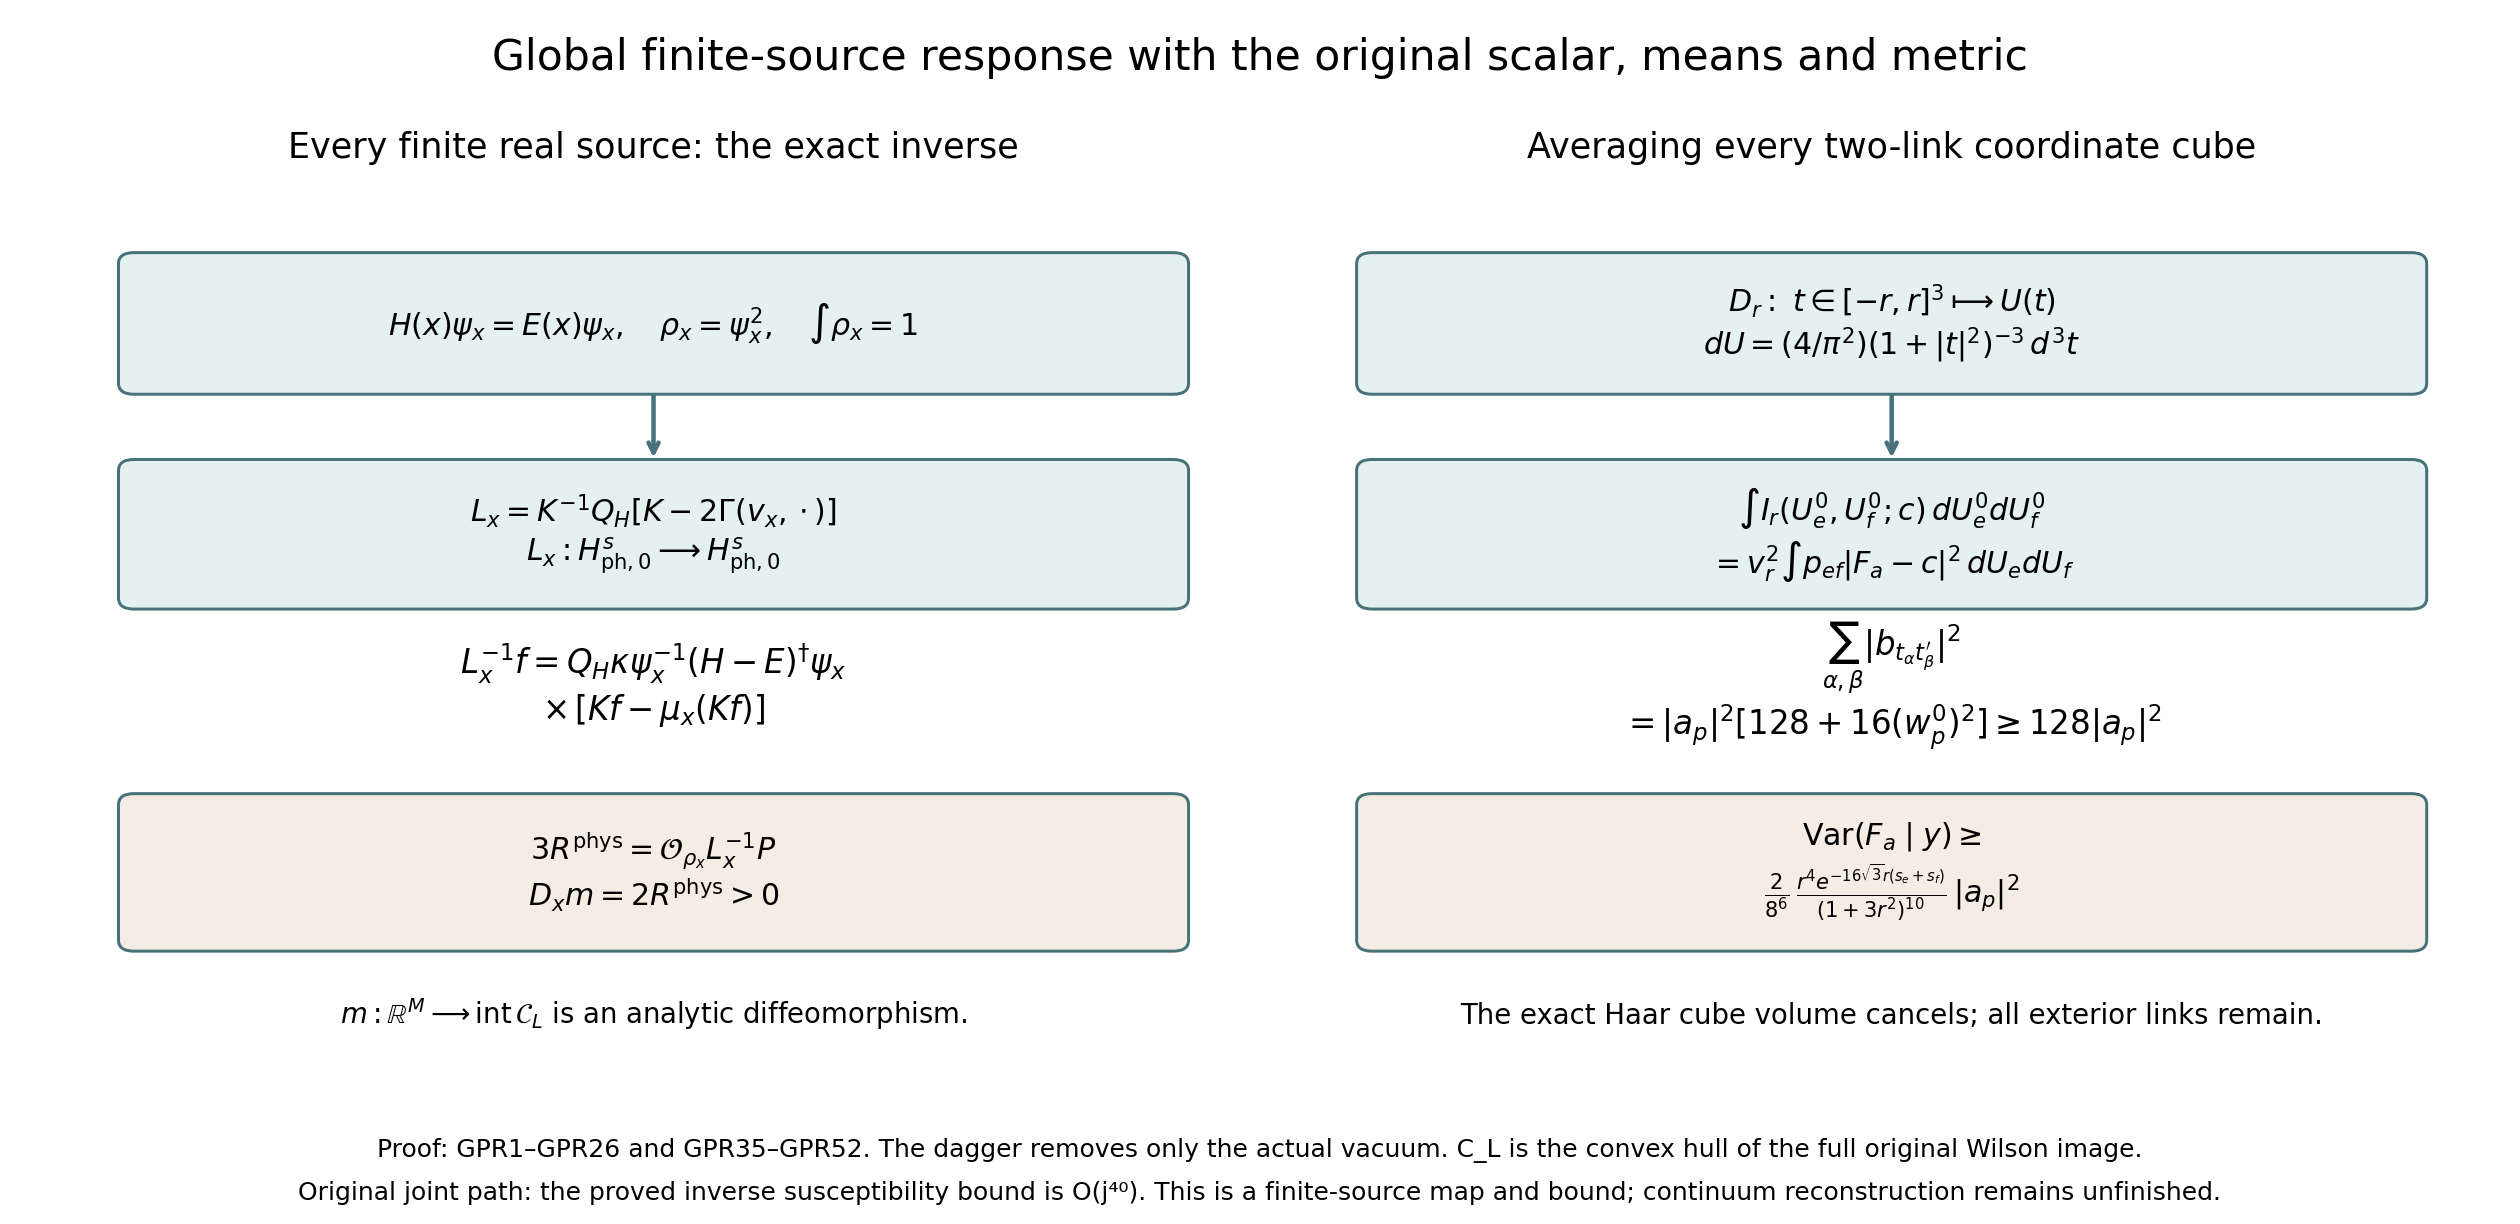
\includegraphics[width=\linewidth,height=.72\textheight,keepaspectratio]{GLOBAL_PHYSICAL_RESPONSE.png}\caption{Exact physical source inverse, observation map and all-centres conditional averaging. Proofs GPR1–GPR26 and GPR35–GPR52; original domains, means, scalars and Haar factors retained.}\end{figure}
\end{document}
